\documentclass[12pt]{memoir}
\usepackage{hyperref}

\usepackage{graphicx}
\usepackage{color}
\usepackage{fancyvrb}
\usepackage{pastie}

\usepackage{amsthm, amsmath, amssymb, amsfonts, mathrsfs}
\usepackage{natbib}
\bibpunct{(}{)}{,}{s}{}{}

\renewcommand{\topfraction}{0.85}
\renewcommand{\textfraction}{0.1}

\renewcommand{\bibname}{References}

% Different font in captions
\captionnamefont{\small\sffamily}
\captiontitlefont{\small\sffamily}
\makeatletter
\renewcommand{\fnum@figure}[1]{\textbf{\figurename~\thefigure}
--- \sffamily}
\makeatother

% applications graphics folder
\graphicspath{{./applications/}}

%%%%%%%%%%%%%%%%%%%%%%%%%%%%%%%%%%%%%%%%%%%%%%%%%%%%%%%%%%%%%%%%%%%%%%%%
\usepackage{color}
\newcommand{\doublecheck}[1]{#1}
\renewcommand{\doublecheck}[1]{\colorbox{yellow}{#1}}

\newcommand{\cc}{\colon\thinspace}

\newcommand{\scA}{\mathcal{A}}
\newcommand{\scB}{\mathcal{B}}
\newcommand{\scC}{\mathcal{C}}
\newcommand{\scD}{\mathcal{D}}
\newcommand{\scE}{\mathcal{E}}
\newcommand{\scF}{\mathcal{F}}
\newcommand{\scG}{\mathcal{G}}
\newcommand{\scO}{\mathcal{O}}
\newcommand{\scX}{\mathcal{X}}
\newcommand{\scY}{\mathcal{Y}}

\newcommand{\bfd}{\mathbf{d}}
\newcommand{\bfr}{\mathbf{r}}
\newcommand{\bfS}{\mathbf{S}}
\newcommand{\bfx}{\mathbf{x}}
\newcommand{\bfy}{\mathbf{y}}
\newcommand{\1}{\mathbf{1}}
\newcommand{\0}{\mathbf{0}}

\newcommand{\bbQ}{\mathbb{Q}}
\newcommand{\bbR}{\mathbb{R}}
\newcommand{\bbZ}{\mathbb{Z}}

\newcommand{\Ot}{\tilde{O}}
\newcommand{\Tt}{\tilde{\Theta}}
\newcommand{\Mt}{\tilde{\Omega}}

\newcommand{\given}{\;|\;}
\newcommand{\biggiven}{\;\big|\;}
\newcommand{\bigggiven}{\;\bigg|\;}

\newcommand{\poly}{\operatorname{poly}}
\newcommand{\Bi}{\operatorname{B}}
\newcommand{\area}{\operatorname{area}}
\renewcommand{\Pr}{\mathbf{P}}
\newcommand{\E}{\mathbf{E}}
\newcommand{\RMSE}{\operatorname{RMSE}}
\newcommand{\dens}{\mathbf{p}}
\renewcommand{\d}{\mathbf{d}}
\newcommand{\logit}{\operatorname{logit}}
\newcommand{\probit}{\operatorname{probit}}

\newcommand{\GammaDist}{\operatorname{Gamma}}
\newcommand{\Poisson}{\operatorname{Poisson}}
\newcommand{\Beta}{\operatorname{Beta}}
\newcommand{\Normal}{\operatorname{Normal}}
\newcommand{\MVNormal}{\operatorname{MVNormal}}
\newcommand{\NegativeBinomial}{\operatorname{NegativeBinomial}}
\newcommand{\Uniform}{\operatorname{Uniform}}
\newcommand{\NBRate}{\operatorname{NBRate}}
\newcommand{\Matern}{\operatorname{Matern}}
\newcommand{\GP}{\operatorname{GP}}
\newcommand{\clip}{\operatorname{clip}}

\newcommand{\true}{\text{true}}
\newcommand{\sex}{\text{sex}}
\renewcommand{\year}{\text{year}}
\newcommand{\regions}{\text{regions}}
\newcommand{\median}{\text{median}}
\newcommand{\CSMR}{\text{CSMR}}
\newcommand{\with}{\text{with}}
\newcommand{\all}{\text{all}}

\def\calC{\mathcal{C}}
\def\calD{\mathcal{D}}

\def\boldpi{{\boldsymbol{\pi}}}
\def\boldw{{\mathbf{w}}}
\def\boldmu{\boldsymbol{\mu}}
\def\boldgamma{\boldsymbol{\gamma}}
\def\boldsigma{\boldsymbol{\sigma}}

\def\PLGP{\operatorname{PLGP}}
\def\PCGP{\operatorname{PCGP}}

\def\a{\alpha}
\def\b{\beta}
%\def\d{\delta}
\def\D{\Delta}
\def\e{\epsilon}
\def\f{\phi}
\def\g{\gamma}
\def\G{\Gamma}
\def\k{\kappa}
\def\la{\lambda}
\def\K{\Kappa}
\def\z{\zeta}
\def\th{\theta}
\def\Th{\Theta}
\def\l{\lambda}
%\def\L{\Lambda}
\def\m{\mu}
\def\n{\nu}
\def\p{\pi}
\def\P{\Pi}
\def\r{\rho}
\def\R{\Rho}
\def\s{\sigma}
\def\S{\Sigma}
\def\t{\tau}
\def\om{\omega}
\def\Om{\Omega}

\newcommand{\proofstart}{{\bf Proof\hspace{2em}}}
\newcommand{\proofend}{\hspace*{\fill}\mbox{$\Box$}}



\begin{document}
\tableofcontents
\chapter{Introduction}
This book, \emph{Integrated Meta-regression Framework for Descriptive
  Epidemiology} is a full-length treatment of new meta-analytic
methods for descriptive epidemiology.  From first principles, it
develops the integrative systems model which constitutes the
theoretical foundation of years lived with disability (YLD) estimation
in burden of disease studies like the Global Burden of Disease 2010
Study (GBD 2010 Study).  The estimation approach relies on producing
age-specific prevalence estimates of the non-fatal outcomes of a vast
array of diseases, injuries, and risk factors.  As part of the GBD
2010 Study, we have developed a Bayesian meta-regression tool
specifically for this purpose. This tool estimates a generalized
negative binomial model for all the epidemiological data with various
types of fixed and random effects.  These include age fixed effects,
fixed effects for covariates that predict country variation in the
quantity of interest, fixed effects that predict variation across
studies due to attributes of the study protocol, and super region,
region and country random intercepts.  The tool uses Bayesian
inference of the parameters to sample from the joint posterior
distribution of model, incorporating all relevant descriptive
epidemiological data.  This approach is new, but the line of research
builds on work in generic disease modeling that has been in use for
almost 20 years in global health
epidemiology.\cite{Barendregt_Generic_2003} However, until now, the
description of the models and the methods have been scattered through
the scientific literature in a loose collection of journal articles,
burden of disease reports, and operations manuals.

This book substantially extends the previous modeling efforts for YLD estimation
in Burden of Disease estimation, by formally connecting a system dynamics model of disease
progression to a statistical model of epidemiological rates, the kind
that are calculated in descriptive epidemiological research and
collected together in a systematic review.  This combination of
systems dynamics modeling and statistical modeling, which I call
\emph{integrative systems modeling} allows the model to integrate all
available relevant data.  Because of the advanced numerical algorithms needed to fit these complex models, a section of the book provides the
necessary background on Markov chain Monte Carlo (MCMC) and other
relevant computational methods.

Experience with the results of systematic review indicates that when
all available relevant data are collected, they are often very
\emph{sparse} and very \emph{noisy}.  In GBD estimation, data sparsity
often means that there are whole regions of the globe for which no
data is available.  Sparse data mean that predictions of prevalence
need to take advantage of relationships to covariates in the
meta-regression or default to the average of a region, super-region or
the world.  Noisy data is an additional challenge. In the regions or
countries with multiple measurements, the results are often highly
heterogeneous. The degree of heterogeneity is far beyond what is
expected on the basis of sampling error and indicates considerable
non-sampling variance.  The sources of non-sampling variance include
sample design, implementation issues in data collection, case
definitions, and diagnostic technologies.

There are a number of other common challenges in estimating the
prevalence of non-fatal outcomes of disease, which are also addressed
in the new framework.
\begin{itemize}
\item Published studies often use non-standard age-groups like 18-35
or 15 and above.  For the GBD, we need to use data from many different
non-standard age-groups to generate coherent estimates for the 20
age-groups for the study.  Given that prevalence for most sequelae are
strongly related to age, this issue is particularly important.

\item Data for conditions are collected for many different outcomes
such as incidence, prevalence, remission, excess mortality or
cause-specific mortality.  The mix of data varies across diseases and
across regions for a disease.  All of these sources provide some
relevant information for estimating prevalence but more often than not
are not strictly comparable due to variations in case definition or
other methodological differences.

\item Within regions or
countries, the true prevalence for a sequela can vary enormously. The
high level of hepatitis C in Egypt is an example in the Middle-East
and North Africa region.  Such within-region heterogeneity in the true
rates must be accommodated in a meta-regression framework.

\item Based on biology, exposure or clinical series, we may have strong
priors on the age pattern of incidence or prevalence for a condition;
for example, we expect the incidence of many cancers to increase with
age due to cumulative exposure to carcinogens at least until some
adult age.  Other examples include no bipolar disorder at very young
ages.  

\item For many conditions the available studies use
different case definitions.  The review of diabetes prevalence studies
identified 18 different case definitions in use.  If all non-reference
definition data are excluded, predictions can be based on an extremely
limited number of studies only.  An alternative is to empirically
adjust (“cross-walk”) between different definitions using the overlap
in available studies.
\end{itemize}

The statistical model developed in this book focuses
particularly on techniques for handling sparse, noisy data, as well as
addressing these additional challenges.  The book explores statistical
models for overdispersed count data, covariate modeling to explain
systematic variation in epidemiological data and increase predictive
accuracy for estimates where no data are available, and age-pattern
modeling to systematically incorporate expert knowledge about how
epidemiological rates vary as a function of age.  It also develops a
novel theory of age-group modeling to address heterogeneity in age
groups commonly found during systematic review.

The theoretical foundations of integrative systems modeling of disease
in populations consititute the first half of this book.  The second
half of the book contains a series of applications of the model to the
meta-analysis of more than a dozen different diseases.  These
practical applications demonstrate how the model performs in a variety
of scenarios. They also investigate how the model performs when the
model assumptions are violated.


\section{Systematic review and meta-analysis}
TK History of systematic review and meta-analysis, from antiquity and
tracing its rise in prominanace in the medical sciences, togrether
with a justifi caion for its continuted practice, in terms of
summarizing the vast quantity of primary researech being
conducted. Distinguish systematic review from meta-analysis, following
the distinction made by PRISMA.

Wikipedia \url{http://en.wikipedia.org/wiki/Systematic_review}
\begin{quote} A systematic review is a literature review
  focused on a research question that tries to identify, appraise,
  select and synthesize all high quality research evidence relevant to
  that question. Systematic reviews of high-quality randomized
  controlled trials are crucial to evidence-based medicine.[1] An
  understanding of systematic reviews and how to implement them in
  practice is becoming mandatory for all professionals involved in the
  delivery of health care. Besides health interventions, systematic
  reviews may concern clinical tests, public health interventions,
  adverse effects, and economic evaluations.[2] Systematic reviews are
  not limited to medicine and are quite common in other sciences such
  as psychology, nursing, occupational therapy, physical therapy,
  educational research, sociology and business management.

A systematic review aims to provide an exhaustive summary of
literature relevant to a research question. The first step of a
systematic review is a thorough search of the literature for relevant
papers. The Methodology section of the review will list the databases
and citation indexes searched, such as Web of Science and PubMed, as
well as any individual journals. Next, the titles and the abstracts of
the identified articles are checked against pre-determined criteria
for eligibility and relevance. Each paper may be assigned an objective
assessment of methodological quality using the Jadad scale or similar
rating system.[3][4][5] Systematic reviews often, but not always, use
statistical techniques (meta-analysis) to combine results of the
eligible studies, or at least use scoring of the levels of evidence
depending on the methodology used. Systematic review is often applied
in the biomedical or healthcare context, but it can be applied in any
field of research. Groups like the Campbell Collaboration are
promoting the use of systematic reviews in policy-making beyond just
healthcare.

A systematic review uses an objective and transparent approach for
research synthesis, with the aim of minimizing bias. While many
systematic reviews are based on an explicit quantitative meta-analysis
of available data, there are also qualitative reviews which adhere to
the standards for gathering, analyzing and reporting evidence. The
EPPI-Centre has been influential in developing methods for combining
both qualitative and quantitative research in systematic reviews.[6]

Many healthcare journals now publish systematic reviews, but the
best-known[citation needed] source is The Cochrane Collaboration, a
group of over 28,000 specialists in health care who systematically
review randomised trials of the effects of prevention, treatments and
rehabilitation as well as health systems interventions. When
appropriate, they also include the results of other types of
research. Cochrane Reviews are published in The Cochrane Database of
Systematic Reviews section of The Cochrane Library. The 2010 impact
factor for The Cochrane Database of Systematic Reviews was 6.186, and
it was ranked 10th in the ``Medicine, General \& Internal'' category.[9]


\end{quote}

Wikipedia \url{http://en.wikipedia.org/wiki/Meta-analysis}
\begin{quote}
In statistics, a meta-analysis combines the results of several studies
that address a set of related research hypotheses. In its simplest
form, this is normally by identification of a common measure of effect
size, for which a weighted average might be the output of a
meta-analyses. Here the weighting might be related to sample sizes
within the individual studies. More generally there are other
differences between the studies that need to be allowed for, but the
general aim of a meta-analysis is to more powerfully estimate the true
``effect size'' as opposed to a smaller ``effect size'' derived in a
single study under a given single set of assumptions and conditions.

Meta-analyses are often, but not always, important components of a
systematic review procedure. Here it is convenient to follow the
terminology used by the Cochrane Collaboration,[1] and use
``meta-analysis'' to refer to statistical methods of combining
evidence, leaving other aspects of 'research synthesis' or 'evidence
synthesis', such as combining information from qualitative studies,
for the more general context of systematic reviews.

The term ``meta-analysis'' was coined by Gene V. Glass.[2]

The first meta-analysis was performed by Karl Pearson in 1904, in an
attempt to overcome the problem of reduced statistical power in
studies with small sample sizes; analyzing the results from a group of
studies can allow more accurate data analysis.[3][4] However, the
first meta-analysis of all conceptually identical experiments
concerning a particular research issue, and conducted by independent
researchers, has been identified as the 1940 book-length publication
Extra-sensory perception after sixty years, authored by Duke
University psychologists J. G. Pratt, J. B. Rhine, and associates.[5]
This encompassed a review of 145 reports on ESP experiments published
from 1882 to 1939, and included an estimate of the influence of
unpublished papers on the overall effect (the file-drawer
problem). Although meta-analysis is widely used in epidemiology and
evidence-based medicine today, a meta-analysis of a medical treatment
was not published until 1955. In the 1970s, more sophisticated
analytical techniques were introduced in educational research,
starting with the work of Gene V. Glass, Frank L. Schmidt and John
E. Hunter.

Gene V Glass was the first modern statistician to formalize the use of
meta-analysis, and is widely recognized as the modern founder of the
method. The online Oxford English Dictionary lists the first usage of
the term in the statistical sense as 1976 by Glass.[2][6] The
statistical theory surrounding meta-analysis was greatly advanced by
the work of Nambury S. Raju, Larry V. Hedges, Harris Cooper, Ingram
Olkin, John E. Hunter, Jacob Cohen, Thomas C. Chalmers, Robert
Rosenthal and Frank L. Schmidt.

\end{quote}

TK a discussion of the common cautions about comparing apples and
oranges in meta-analysis; quote from Cochrane Handbook
\url{http://www.cochrane-handbook.org/}.  But comparing apples and
oranges is exactly what we want to do sometimes, for example when
estimating population levels of nutritional risk factors, where
respondants are asked, ``how many servings of fresh fruits and
vegetables do you eat in a day?''

These concerns are not without grounds, however.  And the purpose of
this book is to develop a method for comparing the results of
descriptive epidemiological studies of disease prevalence, incidence,
remission, and mortality risk, which are focused on subpopulations
from varying age groups, sexes, regions, and time periods.  It is not
impossible, but it is not as easy as inverse variance weighting or
even random effects regression.

It is not without precedent, however.  The next section discusses the
legacy of ``generic disease modeling'', which my integrative approach
to descriptive epidemiological meta-analysis builds upon.



\section{History of generic disease modeling}

The line of research into disease modeling for descriptive
epidemiology has been accompanied by software implementations since
the 1990s.  The development and refinement of these computer codes
provides conveniently named milestones through the history of the
approach.  For example, DisMod I was software developed in the early
1990s to support analysis in the original Global Burden of Disease
Study.  Computing power has increased dramatically over the 20-year
period in which the DisMod family of generic disease modeling software
has evolved, and the aspiration of methods has expanded as well. We
now trace how the approach has evolved from a simple spreadsheet model
to a robust meta-regression framework.

The precursor to the first DisMod, the Harvard Incidence-Prevalence
(HIP) Model, was a spreadsheet implemented in Lotus 123.
\cite{Murray_Quantifying_1994} This model took as input a set of
instantaneous incidence, remission, and excess mortality rates for $5$
age groups, and produced estimates of disease prevalence and duration.
The model involved constructing a life table to simulate a cohort
exposed to a set of age-specific incidence, remission, case fatality
and background mortality hazards. At each year in the life table, the
model simulated a simple 3-compartment model to provide estimates of
the number susceptible, the number of cases and the number of deaths
to input into the life table for the next year.  It was used primarily
for three purposes: to find prevalence for conditions where incidence
is known and reasonable assumptions about remission and excess
mortality can be made; to find attributable deaths that were not
directly coded to a specific cause; and to find incidence for
conditions where prevalence is known.  The third use case required an
interactive procedure in the HIP model, since the input incidence was
unknown.

As is often the case in science, a very similar approach had been
developed previously by researchers at the International Institute
for Applied Systems Analysis in Austria in the 1970s.\cite{international_institute_for_applied_systems_analysis._estimation_1977} This work was
part of a broad program to develop a generic Healthcare System Model
to improve management and planning in the health sector. One component
of this model was a computer program to estimate prevalence from
incidence. That program evolved a population
exposed to age-specific incidences of disease and death through time.
Although it was designed specifically for terminal illness, it is
similar to the DisMod line of models in many ways. It was applied to
estimate the prevalence of malignant neoplasm in Austria, France and
Belgium.


Over the course of the first Global Burden of Disease Study, the HIP
Model evolved in DisMod
I.\cite{murray_global_1996}
This was formalized as a four compartment model, and corresponding
system of differential equations.  Like the HIP model, the input to
DisMod I consisted of instantaneous rates for incidence, remission,
and excess mortality, now specified for $9$ age groups.  In addition
to the three use cases from the HIP model, DisMod I was also used to
estimate the average duration of disabling sequelae, as a function of
age.  DisMod I was used iteratively by analysts working on the GBD 1990
study to identify a solution that matched the available data on
prevalence, incidence, remission, excess mortality and cause-specific
mortality.  DisMod I was used to address multiple challenges: mapping
from incidence data to prevalence and vice-versa; assessing the
consistency between incidence, prevalence and cause-specific mortality.

DisMod II moved from forward simulation into the realm of
optimization.  It provided more control over inputs, as well as a a
graphical user interface and comprehensive user manual, making it more
widely usable than previous iterations.\cite{Barendregt_Generic_2003}
In addition to accepting input of instantaneous rates for incidence,
remission, and excess mortality, DisMod II was also capable of using
age-specific prevalence and cause-specific mortality rates, as well as
incidence as a population rate, and duration when it is short (less
than one year).  It also provided an algorithmic method for data
confrontation, wherein the downhill simplex method was used to
minimize the weighted difference between the inputs and the output
predictions.  Although DisMod II included the step towards
optimization, it was not framed as a statistical likelihood estimation
and thus did not generate uncertainty intervals.  To put it another
way, there was not measurement model included, only the model relating
true population rates.

The generic disease modeling approach was distributed without cost by
the World Health Organization (WHO) through the DisMod II software. It
has been used widely in burden of disease studies over the last 10
years. These studies adopted the methodology of the global study, but
aimed to assess burden at a level of detail more relevant for national
policymakers. Nearly $45$ countries have undertaken national or
subnational burden of disease study, including studies in Mexico,
Chile, Colombia and
Mauritius.\cite{Lozano_Burden_1995,republica_de_colombia_ministerio_de_salud_carga_1994,concha_barrientos_carga_1996,Vos_Mauritius_1996}

Despite its wide application, DisMod II has not been without
criticisms.  One methodological concern that emerged from extensive
application of the model centered on the difficultly in producing
consistent estimates that exhibited face validity, for example age
patterns that increased monotonically as a function of age. Despite
strongly held prior beliefs on the part of domain experts, it was not
uncommon for the prediction to show oscillations as a function of age, due
to the contortions that DisMod II would subject rates to in order to
produce consistent estimates as close to the single rate type input
estimates as possible.

Another important challenge in the DisMod II work flow was the
production of single best estimates for at least three independent
rates to be used as input.  Systematic review often finds multiple
measurements of an age-specific rate, and only one could be the input to
DisMod II.  Transforming a large collection of measured values, often
for incommensurate age intervals, to a single best estimate of disease
prevalence was a difficult challenge in analysis that is a necessary
preprocessing step to do meta-analysis with DisMod II.

A third challenge with DisMod II was in producing robust estimates of
parameter uncertainty.  Although the system included a method to
propagate uncertainty in the input parameters through to the output
estimates, this was laborious and rarely used in practice.

Finally, although DisMod II excelled in providing consistent estimates
from the confrontation of inconsistent estimates of several disease
parameters for a single place and time, it was laborious on the part
of the data analyst to produce comparable estimates for a variety of
different places and times. In the Global Burden of Disease (GBD) 2010
Study, there are 21 geographic regions to produce estimates for, at
three different points in time, for males and females. Even an
analysis that is trivial for one region/time/sex becomes burdensome
when it must be replicated $126$ times.

For the GBD 2010 Study, we initiated a complete redevelopment of the
method, continuing the trend towards including more formal inferential
techniques into the estimation process.  The broad principle behind
this approach is what we call integrative systems modeling (ISM) and
can be characterized in two parts: a system dynamics model of process
and a statistical model of data, considered together, so that instead
of doing forward simulation, as is traditionally the case in system
dynamics modeling, the model is used to solve an inverse problem. This
approach is emerging as a powerful approach for developing models that
integrate all available data sources.  ISM, and its intellectual
history, is the topic of the the next section of this chapter.  On top
of the compartmental model initially conceived for the HIP model, we
have layered an age-standardizing negative binomial mixed effects
spline model, which is fit directly to the data extracted in
systematic review using Bayesian methods.  The details of this
approach constitute the bulk of the first half of this book.

%% \section{Integrative systems modeling}
%% \label{intro-ism}
%% A vast body of literature exists on compartmental modeling and its
%% wide applicability to modeling the dynamics of complex systems
%% \cite{Forrester_Principles_1968, Meadows_Thinking_2008,
%%   Bossel_Systems_2007}.  TK more words in the way of a general
%% introduction to this idea.  Something about Forrester's outsider
%% models of epi, something about the introductory textbook in
%% environmental science Consider a spherical cow, etc.

%% \subsection{Compartmental models in epidemiology}
%% In epidemiology, compartmental models are often constructed to
%% simulate infectious disease dynamics.\cite{Anderson_Infectious_1991}
%% The classic Susceptible-Infectious-Recovered (SIR) model evolves a
%% population through a Susceptible compartment to an Infected
%% compartment to a Recovered
%% compartment.\cite{Kermack_Contribution_1927} Infection dynamics are
%% captured by making the amount of mass that moves from the Susceptible
%% compartment to the Infected compartment dependent on the product of
%% the masses in the two compartments. This dependence implies that the
%% number of new infections will increase with the number of current
%% infections. Extensions of this basic model abound.\cite{Daley_Epidemic_2001,Brauer_Mathematical_2001} The transition
%% parameters in this class of compartmental models, for instance incidence and
%% remission in the case of the SIR model, are usually set
%% based on extracting point estimates of the parameters from literature
%% reviews. Uncertainty is usually assessed based on a sensitivity
%% analysis that solves the compartmental model for the range of
%% parameter estimates found in the literature (UCLA disease modeler who
%% started latin hypercube sampling) \cite{Nagelkerke_Modelling_2002,
%%   Brandeau_Screening_1993, Broutin_Impact_2010}.

%% In statistical analyses, this estimation approach would often be
%% considered insufficient. Instead, the analyst would attempt to find the
%% parameters that, for instance, maximized the likelihood of a set of
%% data samples of the parameter values. This statistical approach has
%% the advantage that uncertainty can be rigorously quantified and an
%% optimal estimate can be identified based on a transparent model.

%% Combining these approaches is currently the subject of basic research.
%% Statistical inference for mechanistic models can be found in full-information maximum likelihood via optimal filtering (FIMLOF) and ``plug-and-play'' inference methodologies. \cite{peterson_statistical_1980, he_plug_2010, breto_time_2009}

%% Advances in statistical modeling and computation have allowed
%% increasingly sophisticated models to be fit to data. These advances
%% have spawned a new modeling approach that seeks to provide more
%% reliable point estimates and estimates of uncertainty for parameters
%% in compartmental models. This new approach, integrative systems
%% modeling, connects a system dynamics model to a statistical model so
%% that parameters in the system can be estimated in a statistical
%% framework without sacrificing the structure provided by the dynamical
%% model.

%% The analyst building a statistical model has a rich vocabulary with
%% which to describe the data-generating process of interest. Data can
%% come from a range of distributions. Hierarchical data can be expressed
%% via random effects and smooth data through the correlation structure
%% of a covariance matrix. In the most mature forms of integrated systems
%% modeling, this rich vocabulary is made available for estimating
%% parameters in a compartmental model. My approach to the meta-regression of descriptive epidemiological data is a prime example of
%% connecting a sophisticated statistical model to a mechanistic model of disease progressing
%% through a population. The complexity of the statistical model and the
%% complexity of the underlying system dynamics model vary across
%% different applications.

%% \subsection{Compartmental models in pharmacokinetics}
%% The field of pharmacokinetics and pharmacodynamics (PK/PD) provides
%% some of the most sophisticated examples of connecting a statistical
%% model to a compartmental model.

%% Pharmacokinetics is the study of how drugs get absorbed and
%% distributed in the body. Pharmacodynamics is the study of the effect
%% of drugs on the body. Much of the content of these two fields overlap
%% so they are often studied together. Within PK/PD, the field of
%% population pharmacokinetics attempts to understand the sources of
%% variability in drug response among individuals
%% \cite{Yuh_Population_1994}. Because clinical trials provide data on
%% only a small subset of the target patient population and at small
%% sample sizes, it is often difficult to estimate variation among
%% individuals without imposing additional structure on the estimation
%% problem. In 1972, the field of population pharmacokinetics began in
%% earnest when nonlinear mixed effects modeling was proposed as a
%% solution to the limited clinical data
%% \cite{Sheiner_Modelling_1972}. The techniques that have emerged in
%% this field are mathematically identical to those necessary for estimation and prediction
%% in ISM meta-regression. Analysts in
%% population pharmacokinetics connect a random effects model of patients
%% within a study (the statistical model) to a compartmental model that
%% describes the process of a drug's absorption in the body (the system dynamics model).

%% Analogous to the advent of the DisMod software for simulating and
%% estimating generic disease models, many different software packages
%% have arisen to help conduct analyses in population
%% pharmacokinetics. NONMEM, which developed at UCSF, was one of the
%% first.\cite{Beal_NONMEM_2009} SAAM II, a computer tool for the
%% simulation, analysis and modeling of pharmacokinetic data, also allows
%% users to fit compartmental models of the drug response to clinical
%% data using the integrative systems modeling
%% approach.\cite{Barrett_SAAM_1998}

%% TK a little more about this, and its glories.





\section[Need for Confrontation]{The Need For Data Integration and Confrontation in Generic Disease Modeling}

A systematic review of published literature and additional sources for
any disease of interest will reveal a variety of information---the
results of studies conducted for many different reasons, by many
different people, at many different times. When developing estimates
of disease burden, and particularly when trying to estimate Years
Lived with Disability (YLDs) for a burden of disease study, I do not
want to overlook any of the results in this myriad of
information. However, the standard techniques of meta-analysis are
not sufficient for this data fusion challenge.

As we will see in Section~\ref{intro-complete_ex}, a systematic review of Parkinson's disease found 71 data points of prevalence from Spain,
conducted during the period of 1987 through 1999.  However, the age ranges of these
studies varied so significantly that at most, only 13 applied to the
same subpopulation.  The situation is even more complicated when
considering data in a global setting. It is a reasonable hypothesis
that the age patterns of Parkinson's disease are quite similar between different countries, but this assumption may not be valid for other diseases such as hepatitis C.
This book will develop from first principles a
meta-analytical approach to integrate data from different studies,
collected from different geographical regions, different and
overlapping age groups, all at different times, to produce estimates
of age-, time-, sex-, and region-specific epidemiological disease
parameters such as incidence, prevalence, remission, and relative risk
of mortality.

For many diseases, a systematic review will also reveal that multiple,
related disease parameters have been studied and can be analyzed. As
detailed in Section~\ref{intro-complete_ex}, studies measuring the prevalence of
Parkinson's disease are common--660 data points met the
inclusion criteria in a recent systematic review. But studies of
disease incidence have also been conducted, as well as studies of
relative risk of mortality and cause-specific mortality. All of these
estimates are related by a logical requirement of internal
consistency.  A prevalent case of the disease can only exist if there
was an incident event sometime in the past, and the number of
prevalent cases this year can be determined from the number of
prevalent cases last year, after adding in all of the incident cases
and subtracting out all of the deaths and remissions (if there is
remission from the disease under consideration).  This suggests a
fundamental equation of population health, which can be further
refined to take age as well as time into account in a systems dynamics
model with two compartments shown below.

    \begin{figure}[h]
        \begin{center}
            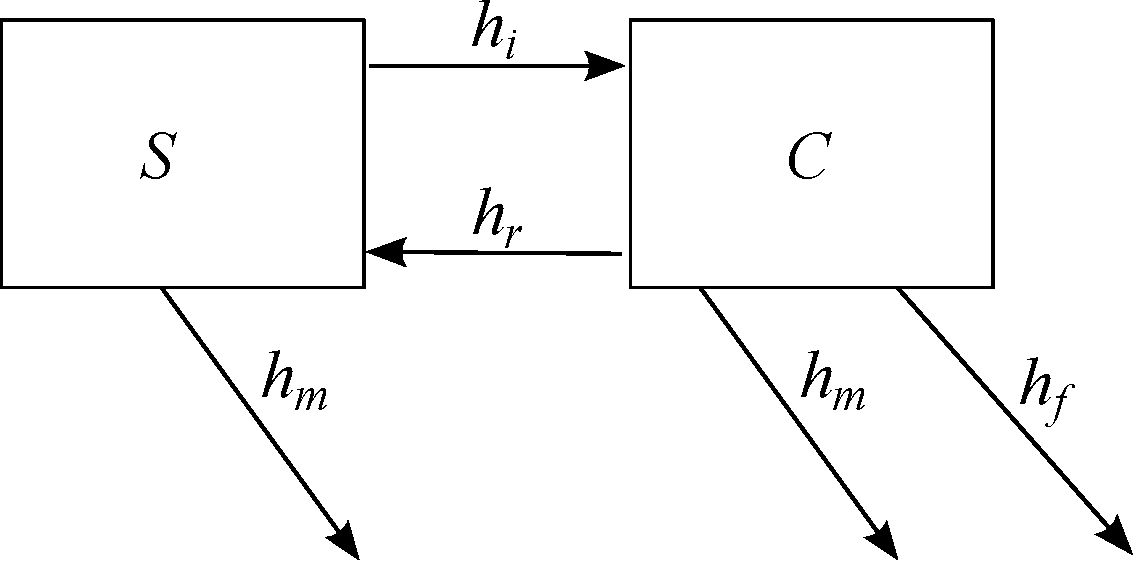
\includegraphics[width=5in]{SC.pdf}
            \caption{The two-compartment model of process for disease in a population, around which the metaregression framework is built. Compartment $S$ contains the population susceptible to the disease and compartment $C$ contains the population with the condition. Individuals move from $S$ to $C$ with incidence hazard $h_i$, and from $C$ to $S$ with remission hazard $h_r$. The susceptible population flows out of the system with without-condition mortality hazard $h_m$, and the with-condition population flows out of the system with with-condition mortality hazard $h_m+h_f$, where $h_f$ is the excess mortality hazard, representing quantitatively the increase in mortality for individuals with the condition.}
            \label{forward-sim-two-compartment}
        \end{center}
    \end{figure}

The precise mathematical representation of this model will be
elaborated on in great detail in
Chapter~\ref{forward-simulation}. Without going into details, it is
intuitive that there must be a relationship between
incidence, prevalence, remission, and with-condition mortality. The
data that has been gathered for each of these epidemiological
parameters should all be brought together in a theoretically grounded
process of data confrontation to produce a best estimate and plausible
uncertainty bounds for disease incidence and prevalence, if this is to
be used in YLD estimation. Through this grand synthesis of a
meta-analysis, I hope to produce the best possible estimates of
disease burden.



\part{Theory}

\section{Introduction and Background}
Integrative systems modeling builds on a larger tradition of system
dynamics modeling, a field that originated out of operations research
and industrial engineering.  System dynamics modeling is an method to
model the behavior of complex systems in terms of stocks, flows, and
feedback loops.  The intuition here is that \emph{stock variables}
quantify the amount of some material, or mass, (or population in
disease modeling) in a compartment at a particular moment in time,
while \emph{flow variables} quantify the amount of material moving
into, out of, or between compartments. The scope of applications for
system dynamics is enormous, and once you start thinking of systems in
this way it may seem that everything can be modeled as stocks and
flows.  This is true of many approaches to modeling, however.  The
scope of system dynamics modeling is vast, and the method is useful
across this vast scope. It has been applied to the study of complex
systems in economics, politics, environmental science, and a diverse
array of other fields.

Traditionally, there is a delineation separating system dynamics
modeling from statistical modeling in the following way: system
dynamics aims to develop a \emph{model of process}, while statistical
approaches focus on developing a \emph{model of data}. Models of
process attempt to explicitly represent the mechanisms behind some
system behavior (deterministically or stochastically), while models of
data often explicitly avoid requiring such mechanistic theories. The
advantage of using the system dynamics approach is that it can
incorporate structural assumptions about the system underlying the
data.  In most applications, however, the process models of system
dynamics and the data models of statistics remain separate.
Integrative systems modeling is an attempt to bring them together for
mutual benefit.

The field of system dynamics has grown out of the work of Jay Forrester, a
management professor at MIT with a background in science and
engineering, in the 1950s. Its first application was in explaining
employment cycles at the company's appliance plants [ref TK]. Managers
incorrectly assumed that cycles merely followed general, economic
cycles, but by developing a compartmental model of the system
underlying GE's appliance business, Forrester showed that the
employment cycles arose from feedback loops inherent to GE's internal
structure. This first application demonstrates a major theme in system
dynamics. In complex systems, determinants of system behavior
considered one-by-one may be insufficient to predict the behavior of
that system. The most important behavior in a complex system arises
out of interactions and feedback between processes in that system. In
the case of disease modeling, the information contained in modeling
the entire disease process of incidence, remission and mortality
can exceed the information contained in separate
analyses of each of these features of the disease epidemiology.

TK paragraph on forward simulation, which includes an simple example,
such as the growth of a population, or use of a renewable resource.

Pharmacokinetic and pharmacodynamic (PKPD) modeling, a subdiscipline
of pharmacology, developed an approach to compartmental modeling in
tandem with system dynamics modeling, largely independently.  However,
the mathematics behind the models of process are extremely
similar. The compartments in PKPD models represent organs and other
physical systems in the body, and stocks represent the quantities of
pharmacologically relevant compounds in these compartments.  The flows
model the process of the drug of interest being metabolized or
otherwise passing through the subject. Mathematically, these models
have precise parallels to the stock-and-flow models developed by
Forrester and colleagues for supply chain analysis. For instance, in
one experiment researchers used a system dynamics approach to model
glucose kinetics. They found that a three compartment model where two
compartments correspond to peripheral pools exchanging plasma at
different rates with a central pool best represented the physiology of
glucose kinetics in their test subjects (in this case, a sample of 7
sheep) [ref TK]. This particular model structure has arisen several
times in applications in pharmacokinetics. It is called the mammillary
model. In another experiment, researchers modeled the kinetics of FULL
NAME TK (EACA) in 6 human subjects. EACA is compound used to control
hemorrhage in patients with bleeding problems. The PKPD researchers
developed a multi-compartmental model, where EACA was infused in a
central compartment, distributed to fast and slow excreting peripheral
compartments, and cleared by two compartments, one representing renal
excretion of the drug, and another representing non-renal excretion
[ref TK]. In both of these examples, and in general practice in
pharmacokinetics, the compartmental model-of-process is connected to a
statistical model-of-data to go beyond forward simulation to develop
methods of statistical inference for compartmental models. This
connection is the central idea of integrative systems modeling, and
one will be developed in detail in later chapters.

There has increasing interest in applying system dynamics principles
to the modeling of health and health systems. Health systems are
particularly complex, with many actors and many feedback loops,
providing a large supply of systems modeling opportunities. The health
of a population is affected by a combination of biological, economic,
demographic, and political forces, and all of these spheres interact
in a unexpected ways. Since the 1970s, system dynamics models have
been applied to model these various forces in order to advance our
understanding of population health [refs TK]. The topics addressed
have included: disease epidemiology, substance abuse epidemiology,
patient flows in emergency care, health care capacity and delivery,
and interactions between health care and disease epidemiology. A
systems approach is often required, because isolating one part of a
public health problem and then addressing that may in fact adversely
affect other parts of the system. For instance, low tar/nicotine
cigarettes were developed to address one part of the burden of disease
caused by tobacco consumption, but consumer behavior was not taken
into account. Consumers tended to take longer, more frequent drags and
thus negated the benefit of the low tar/nicotine content [ref TK]. A
system approach would seek to simultaneously account for both the
effect of the tobacco product on the consumer and the consumer's
behavior. In the context of modeling the progression of a disease
through a population, a model that seems to describe infection
dynamics accurately may conflict with data on remission or
fatality. Only by modeling the three together can the analyst get the
most accurate and consistent estimates.

One area in which public health has a long tradition of compartmental
and system dynamics modeling is in infectious disease [ref Andersen
  and May, Heathecote, Sally Blower, others? see wikipedia
  compartmental models in epi page]. For example, the
Susceptible-Infected-Recovered compartmental model, which was discussed in
Section~\ref{TK}. This basic model has been extended in a variety of
ways in order to model increasingly more complex infectious disease
dynamics. For instance, in one study Nagelkerke and colleagues modeled
the impact of a range of interventions targeted at preventing
transmission of HIV/AIDS epidemics [ref]. They estimated impact using a
compartmental model where the population moved from an Uninfected
compartment to either treated or untreated Infected
compartments to an AIDS compartment to a Death from AIDS
compartment. 

Another example that makes an explicit connection between
epidemiological modeling and system dynamics is the recent work by
Kershenobich and colleagues, who applied a systems approach to
forecasting the prevalence of hepatitis C. They developed a
compartmental model tracking incidence, diagnosis and treatment of the
disease. For the incident population in the model, an individual moves
from an acute phase (which lasts for 6 months) to a chronic phase,
unless that individual is spontaneously cleared of the disease, is
treated and cured or dies. For the prevalent population in the model,
an individual moves from viraemic to non-viraemic, dies or gets
treated and cured. Separate models were also used to estimate the
mortality rate in different countries based on age, liver-related
deaths due to hepatitis C infection, and percent of the population
infected by infection drug users. Sensitivity analyses were conducted
by running the model for a number of input scenarios.  TK description
of what this model allowed the authors to do, and especially how hard
it would have been to do in any other way.

System dynamics has been applied not only to the study of disease
processes, but also the health system. Flaxman and colleagues
developed a stock-and-flow model to synthesize data on the
availability and distribution of insecticide treated bednets (ITNs)
and to predict the proportion of households who owned an ITN. This
analysis employed a Bayesian approach to estimate the parameters of
the compartmental model that describe the process of ITNs moving from
warehouses and other storage facilities into the household and
possibly getting discarded by the households or lost in the
distribution process.



TK connection to the references cited in this NIH RFP for systems modeling
\url{http://grants.nih.gov/grants/guide/pa-files/PAR-08-224.html}
\url{http://ajph.aphapublications.org/cgi/content/full/96/3/452}
\url{http://www.hpsig.com/images/f/f5/SD_background_for_public_health_%284.11.05%29.pdf}
\url{http://www.systemswiki.org/index.php?title=Health_System_Dynamics_References}
\url{http://www.chronicdisease.org/nacdd-initiatives/diabetes/professional-development/act-on-data/SDMResourceList.pdf}

TK review of all pubmed literature that has term system dynamics in
the keywords or something.

TK discussion of bednets model and analogy between this and population
PK approach.

\section{System dynamics model of disease in a population}
At the heart of the new generic disease model is a set of four
compartments representing my fundamental equations of population
health. The compartments represent the population susceptible to the
disease ($S$), the population with the condition ($C$), the population
dead due to other causes ($M$), and the population dead due to the
disease ($D$). The population moves between these boxes following the
arrows shown in the figure, transitioning from $S$ to $C$ with incidence
rate $i$, and from $C$ back to $S$ with remission rate $r$. The susceptible
population transitions into box $M$ with (without-condition) mortality
rate $m$, and the with-condition population transitions into box $M$ with
without-condition mortality rate $m$, and into by $D$ with ``excess
mortality rate'' $f$.

TK parallel between this fundamental model of disease and the demographer's
 basic demographic equation (aka the fundamental balancing equation)
 \url{http://books.google.com/books?id=CR-EXq4y8XAC&lpg=PA5&ots=_jJryixe4z&dq=%22basic%20demographic%20equation%22&pg=PA6#v=onepage&q=%22basic%20demographic%20equation%22&f=false}


\section{Compartmental Model}
\begin{figure}
\begin{center}
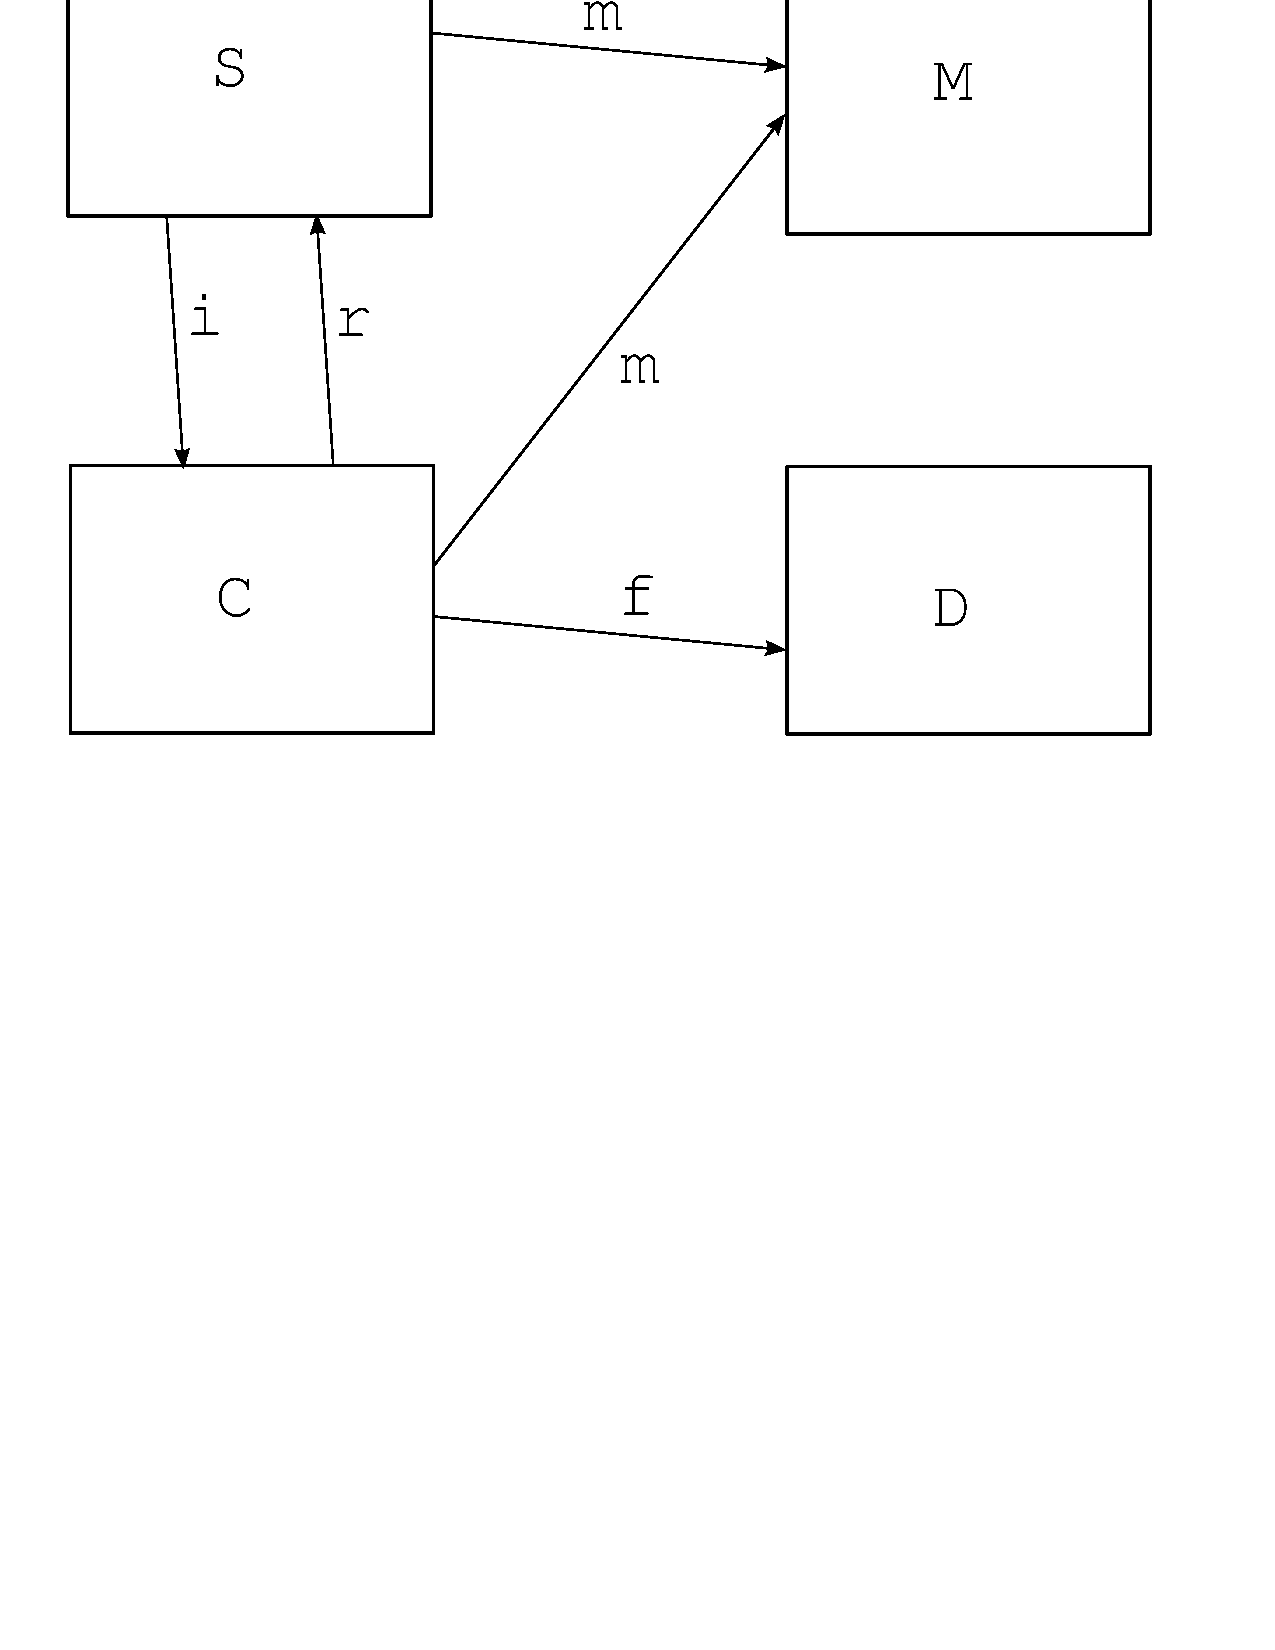
\includegraphics[width=\textwidth]{compartments.pdf}
\end{center}
\caption{TK updated caption; DisMod III uses a 4 compartment model to generate
  age-specific estimates of number without condition ($S$), number
  with condition ($C$), number of deaths not associated with the condition ($M$),
  number of deaths associated with the condition ($D$), incidence rate ($i$),
  remission rate ($r$), without-condition mortality rate ($m$), and
  excess mortality rate ($f$) (all shown in diagram); as well as
  prevalence ($p$), case duration ($X$), relative mortality risk ($RR$), all-cause mortality
  rate ($m_{all}$), and standardized mortality ratio ($SMR$).}
\label{fig:compartmental-model}
\end{figure}

TK Short discussion of what kind of epi study would be designed to
measure each of the important parts of this model. Comment that this
is not always what is available, and the bridge between what we know
and what we want to know will be developed in theory and practice in
several later sections of this book.

Conceptually, it is excess mortality $f$ that has proven hardest to
explain and to understand. This is because in most cases $f$ is a
latent variable, unobservable through most any epi study. Perhaps it
would be clearer to talk about the with-condition mortality rate,
which at least can be measured through a cohort study, and I think
will feel more familiar to the doctor or
epidemiologist. With-condition mortality is $m+f$, and the fact that
$M$ and $D$ are different boxes really is not that important when we
are doing generic disease modeling.

This 4 compartment model is really only a sketch of system dynamics
model I've used however, because it does not show age or time
information. In fact, there are large differences in disease
parameters such as incidence and prevalence as a function of age, and
it is essential for a model to take this into account.  Congenital
abnormalities all have a birth prevalence, while important diseases
such as dementia and Alzheimer's disease have much higher incidence
and prevalence at older ages. Furthermore the incidence and prevalence
of disease, as well as the remission rates and excess-mortality rates
change over time due to shifts in population, changes in prevention or
treatment, or changes in care. And the interdependence between these
factors is complex, but unignorable.  Today's 50-year-olds population
will be tomorrow's 51-year-olds, modulo migration and mortality as
least.

For these reasons, the 4 compartment model is more of a heuristic or
intuitive description of the system dynamics than a precise formal
definition.  A more accurate picture of the system dynamics model
shows the progression of the population as a function of time and age:

TK Time-age expanded version of the compartmental model above.

These figures are not up to the task of giving a full and precise
definition, however, and this is best expressed in terms of a system
of partial differential equations, describing the change in the size
of the compartments as a function of age and time. Although I have
made some simplifying assumptions for practical purposes, I believe
that it is worthwhile to start with the model that I would ideally
like to use, and then simplify it little by little so that it is
appropriately matched to the sparse data and/or the computational
resources available.

TK STOCHASTIC PDE GDM EQUATIONS, an embellishment of the following:

The full model is governed by the following system of partial
differential equations:
\begin{align*}
\frac{\partial S}{\partial (a+t)} &= -(i + m)S + rC,\\
\frac{\partial C}{\partial (a+t)} &= iS - (r + m + f)C,\\
\frac{\partial M}{\partial (a+t)} &= mS + mC,\\
\frac{\partial D}{\partial (a+t)} &= fC,
\end{align*}
where
\begin{align*}
S &= S(a,t) = \text{number without the condition of age $a$ at time $t$}\\
C &= C(a,t) = \text{number with the condition of age $a$ at
  time $t$}\\
M &= M(a,t) = \text{number dead not due to the condition (who would have been) of age $a$ at time
$t$}\\
D &= D(a,t) = \text{number dead due to the condition
  (who would have been) of age $a$ at time $t$}\\[.1in]
i &= i(a,t) = \text{incidence rate for people age $a$ at time $t$}\\
r &= r(a,t) = \text{remission rate for people age $a$ at time $t$}\\
m &= m(a,t) = \text{without-condition mortality rate for people age $a$ at
time $t$}\\
f &= f(a,t) = \text{excess mortality rate for people age $a$ at time
  $t$}
\end{align*}

\subsection{Simplifying assumptions}
\label{theory-forward_sim-compartmental_model-simplying_assumptions}

The first simplification which I have often used is to go from a
stochastic PDE to a deterministic PDE. This was done originally
because of the amount and quality of data available, as well as the
computation speed-up expected.  However, for certain data rich
settings, it may not be desirable. I suspect in the future generic
disease models will want to allow for stochastic PDEs as in the
equations above, and not be tethered by the simplifying assumptions
that I have made here. TK brief discussion of the assumptions inherent
in the deterministic model, and an investigation of how the stochastic
model could deal with these more robustly, for example deviation from
the Markovian assumption that people of age a have the same
with-condition mortality rate, regardless of whether they are a new
case or have had the condition for years. After this simplification,
the system of deterministic PDEs is the following:

\begin{align*}
\frac{\partial S}{\partial (a+t)} &= -(i + m)S + rC,\\
\frac{\partial C}{\partial (a+t)} &= iS - (r + m + f)C,\\
\frac{\partial M}{\partial (a+t)} &= mS + mC,\\
\frac{\partial D}{\partial (a+t)} &= fC,
\end{align*}

The second simplification comes from an assumption that the disease
parameters are not changing substantially with respect to time. TK
implications of simplifying assumptions on time stationarity, and
reduced equation that takes these assumptions into account.  DisMod
III follows the approach used previously, and assumes that the disease
parameters are not changing with time (i.e. the diseases is in endemic
equilibrium),
\[
\frac{\partial S}{\partial t}
=
\frac{\partial C}{\partial t}
=
\frac{\partial D}{\partial t}
=
\frac{\partial M}{\partial t}
=
\frac{\partial i}{\partial t}
=
\frac{\partial r}{\partial t}
=
\frac{\partial m}{\partial t}
=
\frac{\partial f}{\partial t}
=
0.
\]

This assumption on time derivatives is a big one, and deserves careful
assessment. In DisMod II, the default model also included the
assumption that the disease parameters did not change over time, but
an option allowed the model to incorporate assumptions of certain time
trends as well. I will return to the effects of this assumption in
section TK.

The next simplification is on the structure of the rates that dictate
the transitions between compartments (now as a function only of age).
By assuming that these rates are piecewise constant functions of age,
the system of partial differential equations has an explicit solution
for each interval on which the age is constant.

TK rewrite this lead in: Furthermore, DisMod III assumes that the rates are piecewise constant
functions of age, changing rate value only on a specified age mesh.  If
the age mesh is $\{a_0, a_1, \ldots, a_A\}$, then for any $a$ and $a'$
with $a_i \leq a, a' < a_{i+1}$,
\begin{align*}
i(a,t) &= i(a) = i(a')\\
r(a,t) &= r(a) = r(a')\\
m(a,t) &= m(a) = m(a')\\
f(a,t) &= f(a) = f(a')\\
\end{align*}

This permits me to solve the system of equations iteratively, starting
from the first interval, and proceeding interval by interval across
the entire age range. The solution for each age interval, after
assuming that TK FORMAL EQUATOIN OF ASSUMPTION takes the form of a
matrix exponential TK DISPLAY EQUATION.

These assumptions permit DisMod III to solve  explicitly for $S, C, D$
and $M$ iteratively.  The solution is conveniently expressed using the
matrix exponential:
\begin{equation}
\label{eq:ode-soln}
\begin{bmatrix}
S(a_{i+1})\\C(a_{i+1})\\M(a_{i+1})\\D(a_{i+1})
\end{bmatrix}
=
\exp\left(\begin{bmatrix}
-i(a_i)-m(a_i) & r(a_i)             & 0&0 \\
i(a_i)      & -r(a_i) -m(a_i) - f(a_i) & 0&0\\
m(a_i)      & m(a_i)             & 0&0 \\
0        & f(a_i)            & 0&0
\end{bmatrix}
(a_{i+1}-a_i)\right)
\begin{bmatrix}
S(a_i)\\C(a_i)\\M(a_i)\\D(a_i)
\end{bmatrix}
\end{equation}

There is another, related, simplification that is really more a matter
of computational convenience than mathematical simplification.  The
iterative solution to the difference equations above provides the
exact values on an age mesh $\{a_0, a_1, \ldots, a_I\}$, and this
appears in the inner-most loop of the computation, so it is a
significant time saving approximation to use linear interpolation to
fill in prevalence values between the points on the age mesh, instead
of using a more sophisticated differential equation solver to provides
a more precise solution to the system of ODEs. The effects of this
approximation can be minimized by choosing an age mesh appropriately,
and will be examined in more detail qualitatively later in the section
and quantatively in the Chapter TK on numerical algorithms.

Although the primary use of this model is for inference of model
parameters (sometimes called the ``inverse problem''), I can easily
apply it ``forwards'' to show how rates on incidence, remission, and
excess-mortality produce different prevalence curves. The next section
explores this forward simulation through a series of detailed
examples, to build up the reader's intuition around how consistency
forces interrelationships between prevalence, incidence, remission,
and mortality.


\section{Forward simulation examples}

When a generic disease model is initialized with all-cause mortality
data and nothing else, the initial values produce the following set of
consistent age patterns:

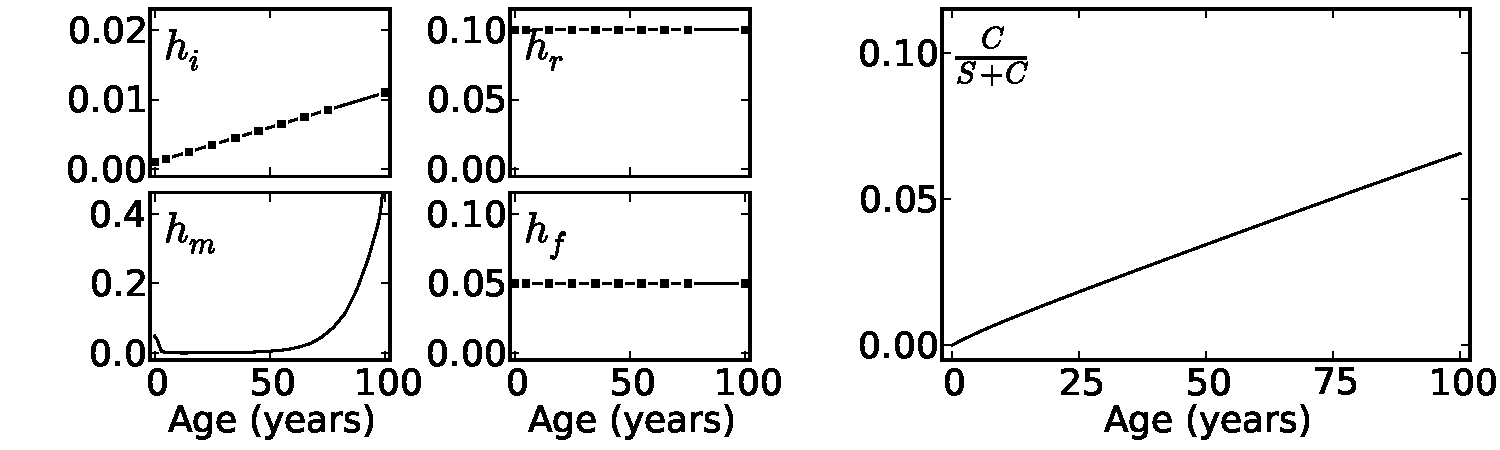
\includegraphics[width=\textwidth]{initial.png}

The next example shows that increasing the remission rate with
incidence and excess mortality unchanged (and all-cause mortality
unchanged as well) leads to a very different age pattern for
prevalence. It is also worth pointing out that since prevalence has
changed with excess mortality and all-cause mortality rates held
constant, the with-condition and background mortality rates have also
changed to maintain consistency.

\includegraphics[width=\textwidth]{more-remission.png}

By changing the incidence rate age pattern to be increasing as a
function of the square root age, I can demonstrate that very similar
prevalence rates are consistent with very different incidence and
remission rates.

\includegraphics[width=\textwidth]{increasing-incidence.png}

Although the prevalence age pattern is largely determined by the
remission, incidence, and mortality rates, the birth prevalence can
also change the shape dramatically.  Here are the results of the same
remission, incidence, and mortality rates as above, but with a birth
prevalence of 20\%.

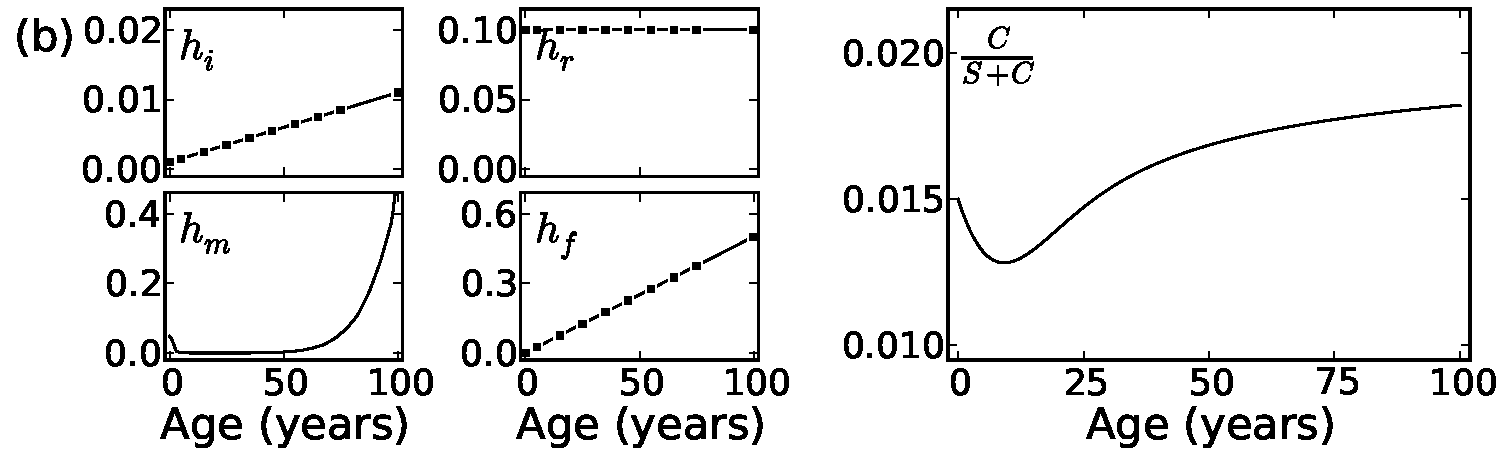
\includegraphics[width=\textwidth]{birth-prevalence.png}

An interesting, and perhaps unexpected feature of this set of
consistent rates above is that when prevalence levels start so high,
the levels remain high during the teenage years, where all-cause
mortality rates are quite low in this population (following the rates
for males in the North American High Income region in 2005), which
produces very low levels of background mortality for these age
groups. In other words, in order for the model to be consistent, it is
necessary to assume that the vast preponderance of teenage deaths are
due to this disease.

Finally, the excess mortality rate (which is the most difficult of the
rates to conceptualize, due to its unobservability) has an effect of
modulating the prevalence that is similar to the remission rate,
although not identical.  The final figure in this series shows the
results of choosing an excess mortality rate to have an age function
equal to ten times the all-cause mortality rate (which is to say a
standardized mortality rate of constant value eleven for all ages).

\includegraphics[width=\textwidth]{higher-smr.png}

The decreasing prevalence after age 65 is worthy of remarking
on. Although the incidence rate is increasing and the remission rate
remains unchanged, having a constant (albeit high) standardized
mortality ratio means that when all-cause mortality rises, the
with-condition mortality rises differentially with such magnitude that
the prevalence of the condition in older populations goes down.

To summarize, this series of figures has shown the intuitive and
less-than-intuitive way that the levels and age patterns of different
epidemiological parameters must be interrelated to satisfy the
fundamental equations of population health (when disease rates for
each age are changing negligibly slowly as a function of time).

The next series of figures continues to build familiarity with the
features of consistent disease modeling, by selecting age patterns for
certain rates based on toy models of a variety of diseases.  For
example, for a disorder like depression, for which there is primarily
incidence in early adulthood, high remission rate, and low excess
mortality, the consistency conditions produce a prevalence age pettern
that peaks at age 25: 

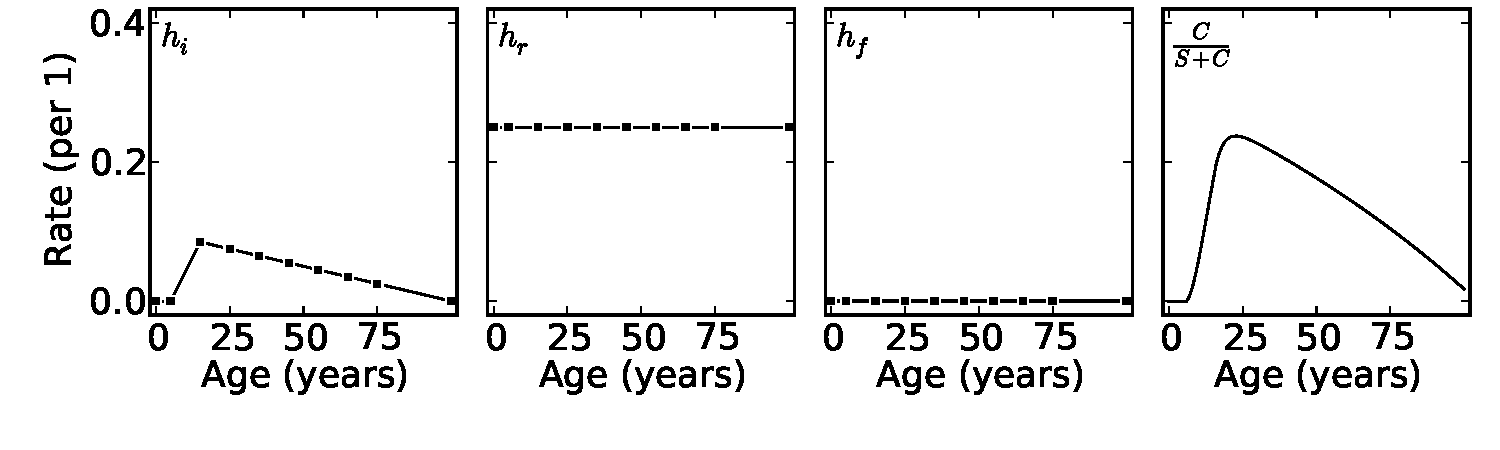
\includegraphics[width=\textwidth]{forward-sim-mental.png}

For a congenital disorder, like TK, with birth prevalence, no
incidence after birth, no remission, and substantial mortality, the
consistent prevalence age pattern is the following:

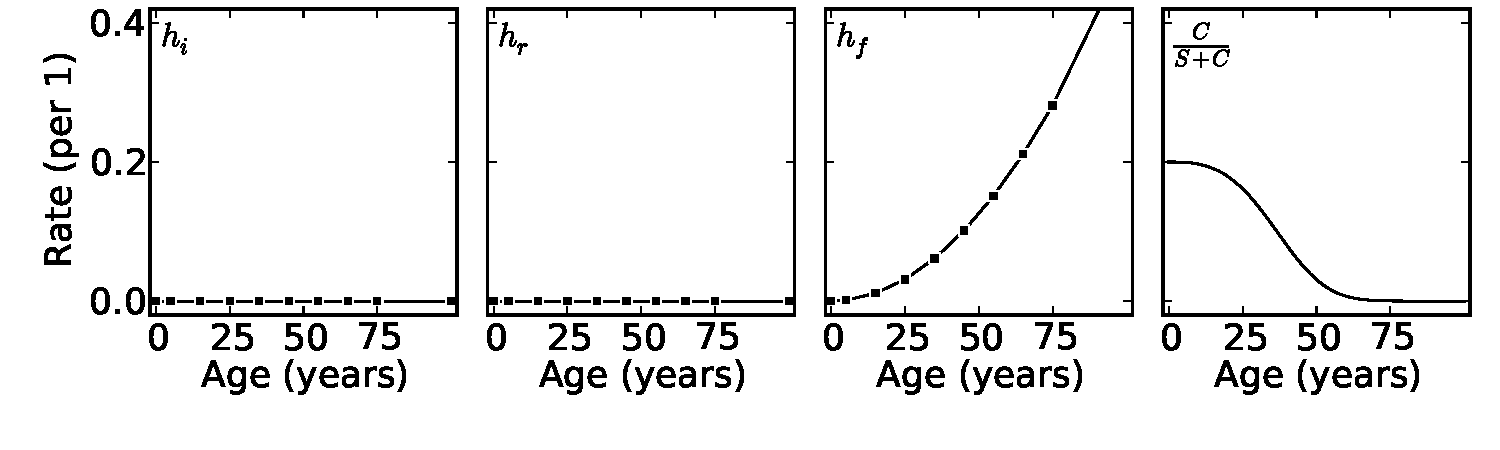
\includegraphics[width=\textwidth]{forward-sim-congenital.png}

For a disorder that affects the elderly, like TK, the consistent age
patterns for mortality, incidence, remission, and prevalence could
look like the following: 

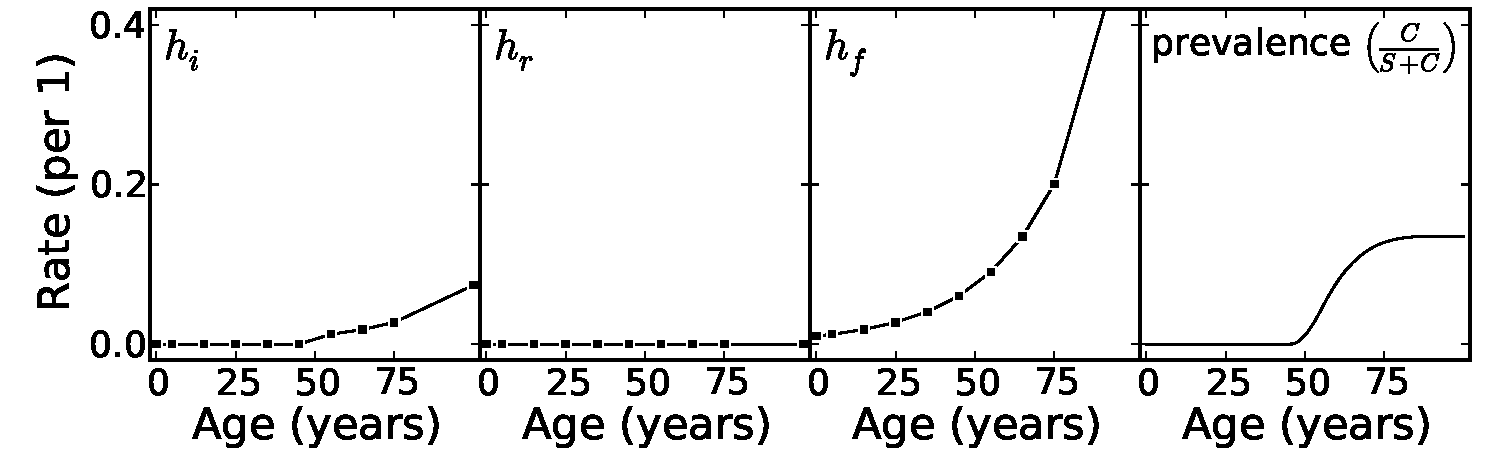
\includegraphics[width=\textwidth]{forward-sim-old_age.png}

And for a disorder related to the reproductive system, like TK, with
substantial excess mortality and incidence during ages 15-60, and
remission that increases substantially at age 55, the consistent age
patterns could look like the following: 

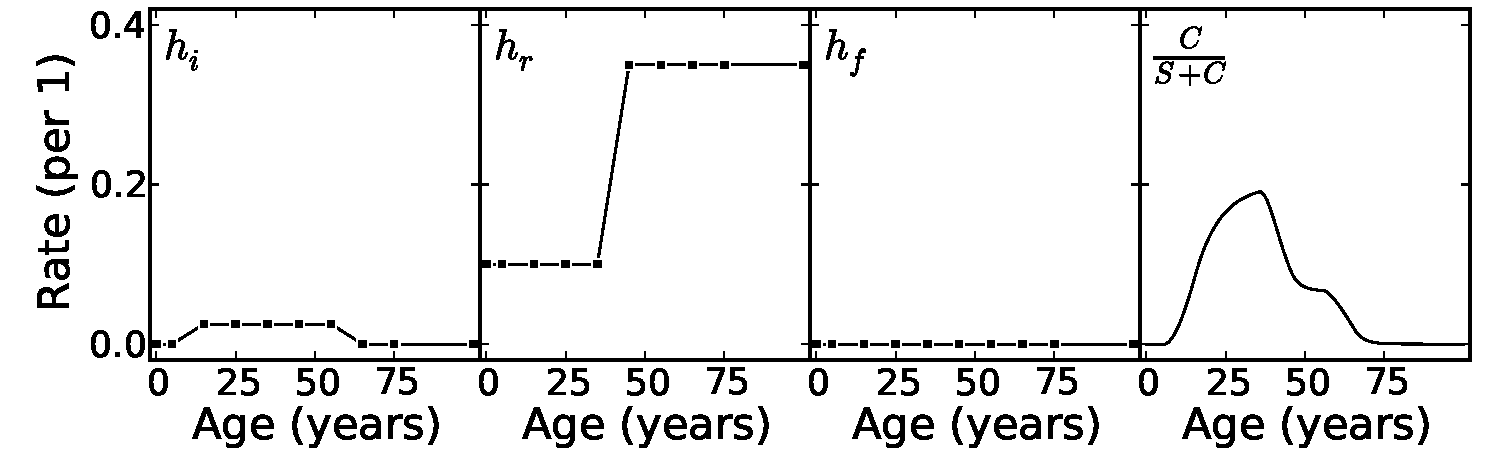
\includegraphics[width=\textwidth]{forward-sim-reproductive.png}

To conclude this series of plots, I've included an "incidence impulse
response" example, showing the prevalence produced to be consistent
with an incidence pattern that is only nonzero for a single age group:

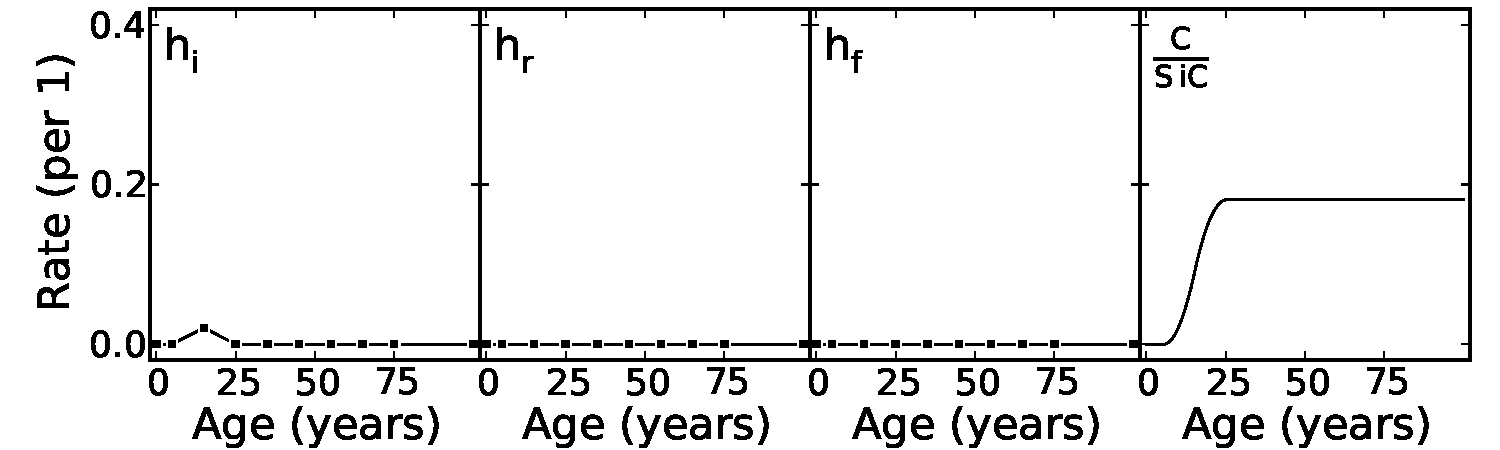
\includegraphics[width=\textwidth]{forward-sim-incidence_pulse.png}

This also provides a mechanism to investigate how wrong the estimates
may become when the assumption that rates are constant over time (for
a given age) is violated. This is the core of my simulation approach
to model validation, to which I will return in section TK.

TK The simulation study approach can be described in full detail here
as well, and can serve as justification for decisions described in the
next two chapters.

\section{What happens to prevalence when the disease incidence or remission or mortality is not constant over time?}

Certain important diseases such as diabetes are widely believed to
have substantial changes in incidence, remission, and mortality rates
over time.  What is the effect of the endemic equilibrium assumption
of the age-specific prevalence. TK plots comparing prevalence from a
synthetic cohort model to a period model using simulation data.

\chapter{Age pattern models}
\label{theory-age_pattern_model}
\chapterprecis{Abraham D. Flaxman}
The rate models of data in the previous chapter need several
extensions to be truly useful in descriptive epidemiological
metaregression.  The most important is representing the differences in
rates as a function of age.  In this chapter, I develop the
mathematical and statistical theory behind a model for age specificity
in prevalence rates as well as other epidemiological hazard functions,
such as incidence, remission, without-condition mortality, and
excess-mortality hazards.

Figure~\ref{ssas-mx_female_1990} shows age-specific all-cause
mortality rates for $5$-year age groups.  These mortality estimates are
for females in Southern sub-Saharan Africa in 1990.  A striking
feature of this plot is the range of variation in mortality levels as
a function of age.  They vary by $850$-fold between the minimum
in the $10$- to $14$-year-olds and the maximum at the oldest
ages. Epidemiological rates also vary among regions, times, and
sexes.  A figure like figure~\ref{ssas-mx_female_1990} for the Asia Pacific,
high income, region in 1990 would look very different, as
would the Southern sub-Saharan Africa region in 2010. However,
systematic variation as a function of \emph{age} is often the largest
source of variation by orders of magnitude, and furthermore, this
variation is often distinctly nonlinear.

\begin{figure}[h]
\begin{center}
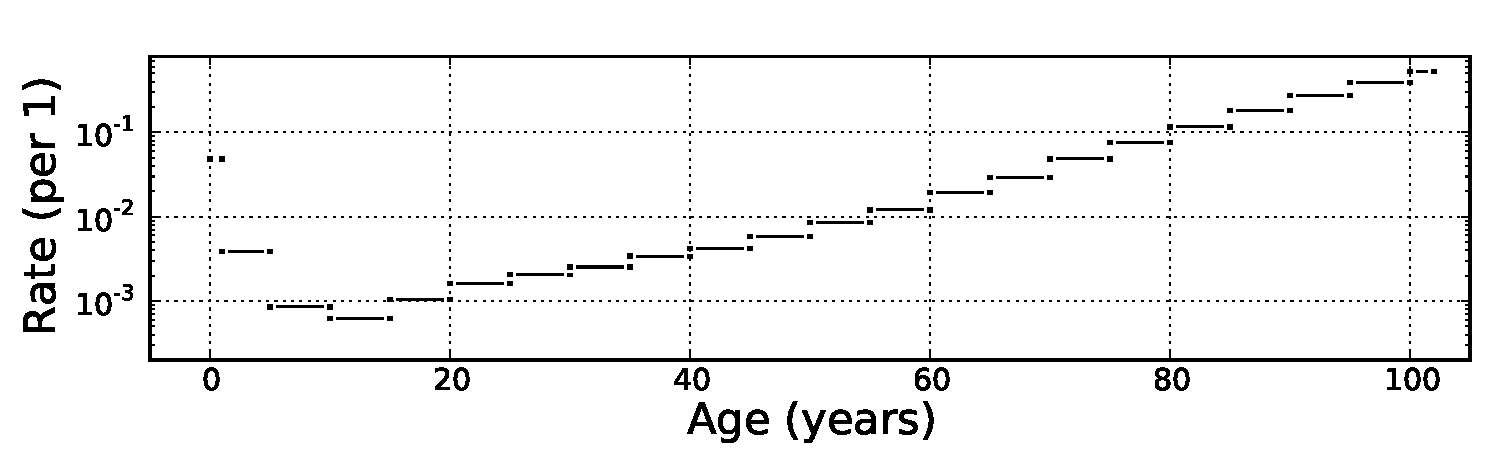
\includegraphics[width=\textwidth]{ssas-mx_female_1990.pdf}
\caption[All-cause mortality as a function of age.]{All-cause mortality for
  females in the Southern sub-Saharan Africa
  region in 1990 as a function of age shows the range of
  variation in age-specific rates.  All-cause mortality is as low as $6$ per
  $10,000$ PY at age $10$ but rises above $5000$ per $10,000$ PY at age $100$.}
\label{ssas-mx_female_1990}
\end{center}
\end{figure}

The approach that I have taken for modeling age-specific hazards draws
on the mathematical theory of spline interpolation and on the
statistical theory of penalized spline regression.  It is developed in
full detail in this chapter.


\section{Definition of spline models}
\label{spline_models}
For my purposes, a spline model can be any piecewise polynomial
function.  Often I will require this function to be continuous, but
not always.  This is a departure from the conventions of statistical
spline modeling, which focuses on continuous and continuously
differentiable splines.\cite{hastie_elements_2009,wahba_spline_1990}

I represent a spline model for an age-specific hazard $h(a)$ by a set
of knots $a_1,\dots,a_{K}$ and a set of piecewise polynomial basis
functions $\{p_1,\ldots,p_{K'}\}$.  Each knot has a corresponding
basis function, and for higher-order splines, there may be additional
basis functions as well, so $K \leq K'$.  The model then has $K'$
parameters, $\gamma_1,\ldots,\gamma_{K'}$, and takes the form
\[
h(a) = \sum_{k=1}^{K'} \gamma_k p_k(a).
\]

The mathematical definition of the model is straightforward, but the
detail of selecting the piecewise polynomials remains to be developed.
This is where the spirit of spline modeling lies. The knots $a_1,
\dots, a_{K}$ partition the age range into intervals. If I make each
piecewise polynomial $p_k(a)$ equal to $1$ on its interval (i.e., when
$a_k \leq a < a_{k+1}$) and $0$ otherwise, this yields a piecewise
constant spline model.  This is an important specialization, the
simplest of my spline models.  Using the notation $\1[a_k \leq a <
  a_{k+1}]$ to denote the function
\[f(a)
= \begin{cases}1,&\quad\text{if }a_k \leq a <
  a_{k+1};\\0,&\quad\text{otherwise;}\end{cases}
\]
 and the convention
that $a_{K+1} = \infty$, I can write out the piecewise constant spline
model as
\[
h(a) = \sum_{k=1}^K \gamma_k \1[a_k \leq a < a_{k+1}].
\]

By taking the piecewise polynomial corresponding to each knot as $0$
before its knot and a linearly increasing function after, the model
specializes to a piecewise linear spline model, a continuous
function that has a constant derivative at all nonknots.  By adding
an additional basis function that is not associated with a knot, this
piecewise linear spline model becomes a flexible approximation for any
nonlinear function and is the main form I have used in representing
age-specific hazards in the work to come.  I can write out the
piecewise constant specialization of the spline model as
\[
h(a) = \gamma_0 + \sum_{k=1}^K \gamma_k a \1[a \geq a_k].
\]

I find that in applications of this model it is useful to represent
the piecewise linear spline in an alternative basis, where the model
parameter $\gamma_k$ represents the values of $h(a_k)$ instead of the
change in the slope at this point.  This yields a more complicated set
of basis functions, but it is not necessary to write out the basis
functions explicitly.


Figure~\ref{splines_fig} shows the results of fitting spline models
for age-specific hazards to simulated data to minimize the sum of the
square differences between the predicted and observed values.  When
the piecewise constant model is fitted, it produces an age-specific
hazard function consisting of a series of horizontal (constant) lines
in each of the intervals between knots.  Interval $k$ has
$\gamma_k$ equal to the mean value of the simulated data between knots
$a_k$ and $a_{k+1}$, which is quite a sensible choice.

A more favorable and flexible fit to the data is achieved by the
piecewise linear spline model, which produces a continuous function
of age as its prediction. In many cases, a piecewise linear fit of
this type is sufficient to capture the nonlinearity in the data, and
this will be the typical model for epidemiological rates in the second
half of this book.  It is possible to go further along this path of
smoothing, however, and splines that have continuous derivatives and
even continuous second derivatives are popular alternatives, achievable
by simply choosing different piecewise polynomials for the basis
functions.


\begin{figure}[h]
\begin{center}
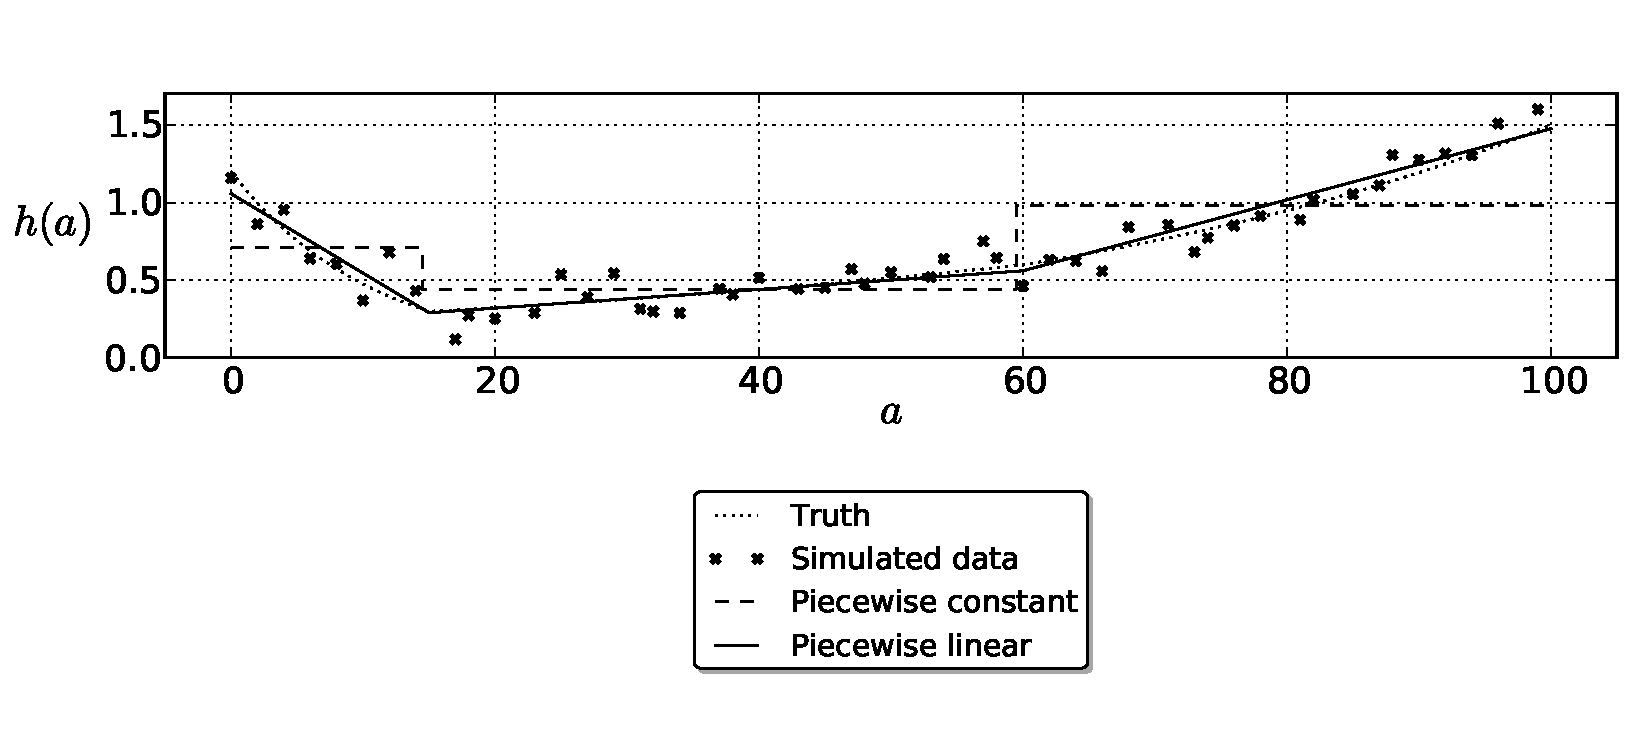
\includegraphics[width=\textwidth]{splines-fig.pdf}
\caption[Spline interpolation of simulated data.]{Spline interpolation
  of simulated data. The true age-specific
  rate is piecewise log-linear, so none of the splines can represent
  it perfectly. The true age-specific rate and the models all have
  knot set $\{0, 15, 60, 100\}$.}
\label{splines_fig}
\end{center}
\end{figure}


\section{Choosing knots}

To this point, I have taken as given the number and location of the
knots in the spline model. However, selecting the number and location
of the knots is an important task, and when working with sparse and
noisy data, this can influence the model results
substantially.

When data are abundant and age patterns are clear, models will not be
very sensitive to the choice of knots.  When data are not abundant, or
when the age patterns are not clear from the data, however, knot
selection is an important part of the modeling process.  In this
setting, knot locations should be chosen a priori, based on expert
knowledge about the disease being modeled. For example, in a recent
study looking at global trends in mean systolic blood pressure as a
function of age, the modelers chose to use a cubic regression spline
with knots located at ages $30$ and $60$.\cite{danaei_national_2011} These
choices reflect the expectation, based on literature and prior
knowledge, that the behavior of mean systolic blood pressure as a
function of age would be distinct in these intervals due to low blood
pressure in young adults and to survivor effects in elderly populations.

Although this approach of using expert knowledge to inform the choice of the number
and location of knots is practical and allows for users to
determine critical features of the model, it is certainly not the only
approach. Much literature is devoted to the choice of knot locations
and the number of knots.
An important direction for future work is to remove the reliance on
expert knowledge to inform knot selection.  This could proceed
through model selection or model averaging of models with a variety of
knot locations, \cite{raftery_bayesian_1997} through
techniques developed in the adaptive regression spline literature,
\cite{friedman_multivariate_1991} or by leaving spline models altogether and using Gaussian
processes or some similar nonparametric model for the age pattern.
\cite{rasmussen_gaussian_2006,diggle_model-based_2010}

\section{Penalized spline models}
One approach to address the challenge of knot selection is to include
more knots in the model and then also include a penalty function to
discourage the model from using the additional knots when the data
do not call for them.  This penalized spline model can be formulated in a
Bayesian framework by introducing a prior that represents the belief that, in
the absence of evidence, the age pattern does not vary.
Mathematically, this takes the form of a penalty on the root mean
square of the derivative of the age-specific rate $h(a)$:
\[
\left[\int _{a=a_1} ^{a_K} \| h'(a) \|^2 \d w(a)\right]^{1/2} \sim N(0, \sigma^2).
\]
This introduces an additional model parameter, $\sigma$, which can be
viewed as a hyperprior and controls the amount of smoothing that the
penalty creates.

For the piecewise linear penalized splines that will be used most
frequently in the second half of this book, the derivative of $h$ is
constant between knots, so, with equal weighting for smoothing at all
ages, the integral above simplifies to the following:
\begin{align*}
\int _{a=a_1} ^{a_K} \| h'(a) \|^2 \d a
& = \sum_{k=1} ^{K-1} \left[\frac{h(a_{k+1}) - h(a_k)}{a_{k+1}-a_k}\right]^2 \frac{a_{k+1}-a_k}{a_K - a_1}\\
&= \sum_{k=1} ^{K-1} \frac{\left[h(a_{k+1}) - h(a_k)\right]^2}{(a_{k+1}-a_k)(a_K - a_1)}.
\end{align*}
Figure~\ref{smoothing-splines} shows the effect of increasing the
smoothing parameter $\sigma$ when many more knots than necessary have been included in the model.

\begin{figure}[h]
\begin{center}
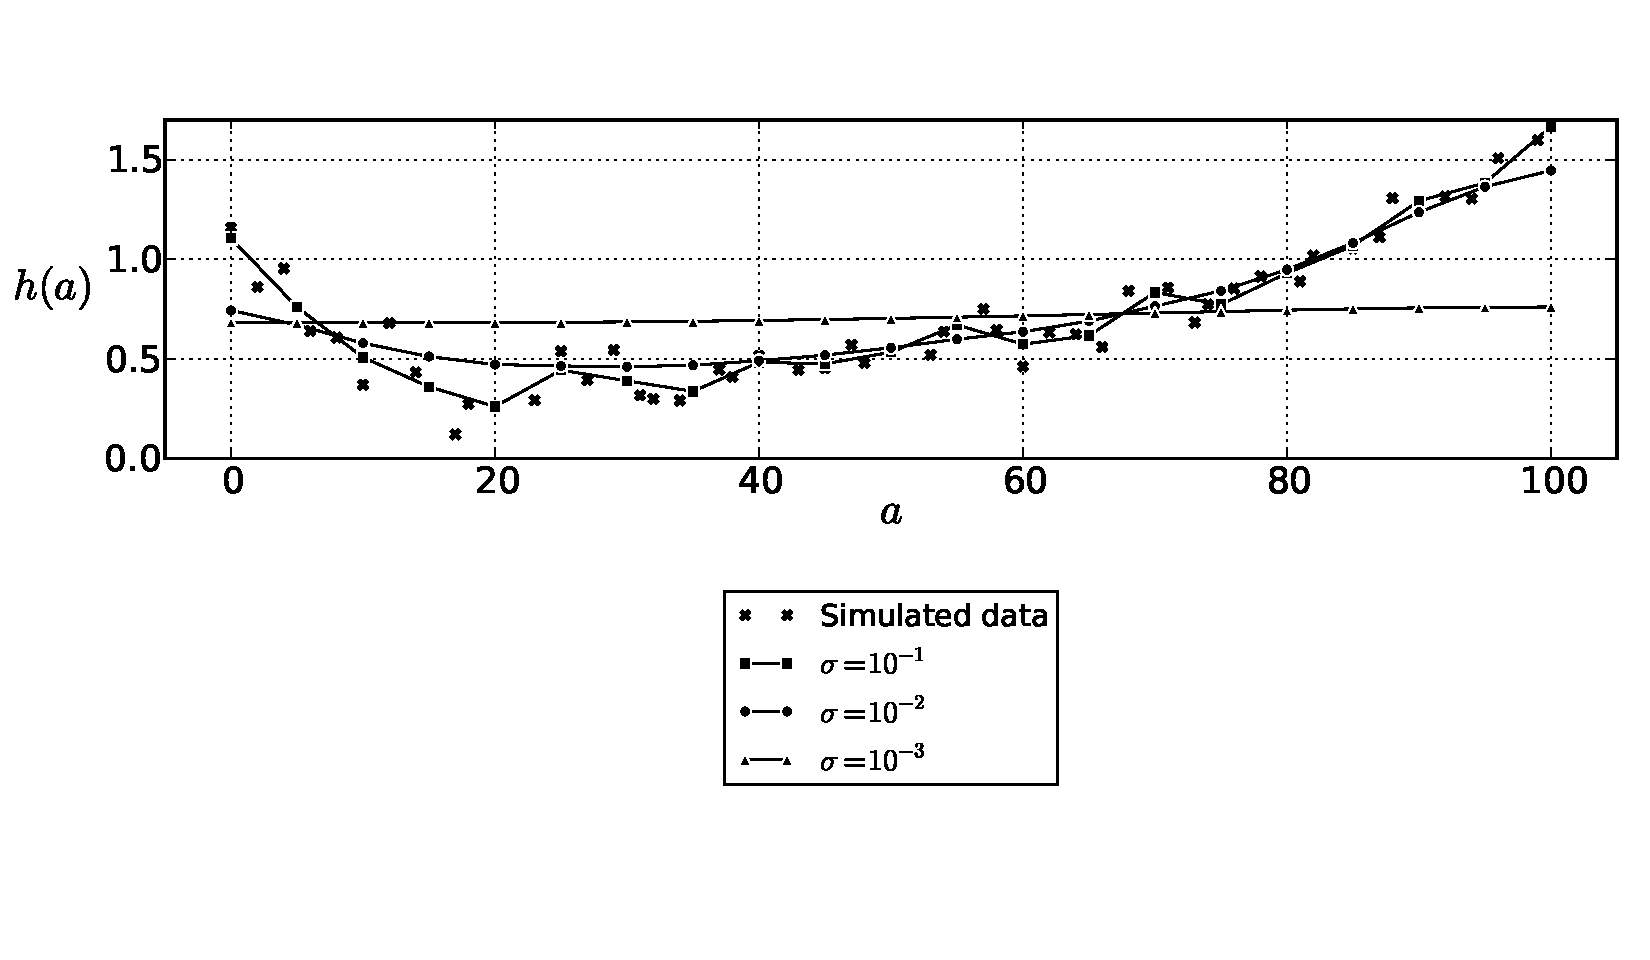
\includegraphics[width=\textwidth]{smoothing-splines.pdf}
\caption[Penalized splines with a carefully chosen smoothing
  parameter.]{Penalized splines with a carefully chosen smoothing parameter
  $\sigma$ provide a solution to the challenge of knot selection in
  spline modeling.  Without smoothing, including many knots leads to
  estimates that are overly uncertain and wiggly.  Smoothing, in the
  form of a quadratic penalty on the derivative of the age pattern,
  allows many knots to be included.  But too much smoothing, for
  example, $\sigma=10^{-3}$ in this case, results in a model that does
  not reflect true patterns in the data.}
\label{smoothing-splines}
\end{center}
\end{figure}


\section{Augmenting the spline model}
There are a few ways to augment the spline model that are useful when
modeling age-specific rates. Since the epidemiological rates I have modeled
are always nonnegative, I have parametrized the spline in
terms of the log of the knot values, so that $h(a)$ is a piecewise
linear spline model with knots $a_1,\ldots,a_K$, and
\[
h(a_k) = e^{\gamma_k}.
\]
To fit the model in a Bayesian framework, I have defaulted to
giving these $\gamma_i$'s ``weakly informative'' priors,
\[
\gamma_i \sim \Normal\left(0, 10^2\right).
\]
This has very little effect on the posterior distribution but makes
the prior ``proper'' and also helps with algorithm convergence in
some instances. Where relevant expert knowledge is
available, I can replace this with a more informative prior (this idea
is elaborated in chapter~\ref{theory-expert_priors}).

Finally, to deal with the order-of-magnitude differences of
age-specific rates, I have applied the smoothing penalty to the
logarithm of the rate rather than to the rate itself.  This creates an additional
complication, however, because the informative priors often say that
rates are $0$ for certain ages.  To avoid the ill effects of
smoothing when the rate contains values of $0$, I have
rounded up any $\gamma_i$ values that are below $10$ times the mean
rate.  The approach is operationalized as a penalty term in the prior:
\[
\widetilde{\|h'\|} = \sqrt{\sum_{k=1}^{K-1}
\frac{\left[\max(\gamma_k, \gamma_{\min})
-
\max(\gamma_{k+1}, \gamma_{\min})\right]^2
}{(a_{k+1}-a_k)(a_K-a_1)}} \sim \Normal(0, \sigma^2),
\]
where
\[
\gamma_{\min} = \log\left[\bigg(\sum_{i=0}^K e^{\gamma_i}/10\bigg)
/ K\right].
\]

Taken all together then, the model for an age-specific hazard function
that will be used in this book is
\begin{align*}
h(a) &= \sum_{k=1}^{K-1} \1[a_k \leq a < a_{k+1}]
\left( \frac{a-a_k}    {a_{k+1}-a_k} e^{\gamma_k}
     + \frac{a_{k+1}-a}{a_{k+1}-a_k} e^{\gamma_{k+1}}\right),\\
\gamma_k &\sim \Normal\left(0, 10^2\right),\\
\widetilde{\|h'\|} &\sim \Normal(0, \sigma^2).\\
\end{align*}
The value of $\sigma$ is a model parameter that will receive a very
informative hyperprior; for example, ``slightly smooth'' is
represented by $\sigma=0.1$.




\chapter{Expert priors on age patterns}
\label{theory-expert_priors}
\chapterprecis{Abraham D. Flaxman}

When dealing with sparse and noisy data, it is sometimes necessary to
include additional expert knowledge on the age pattern of
epidemiological rates.  For example, data sparsity can take the form
of a lack of information about age-specific hazards of disease in children.  In
diseases that are rare or nonexistent in children, the fact that incidence is
effectively $0$ before a certain age is known by disease experts but
not represented in the data collected by systematic review.

A benefit of the Bayesian methods that will be used to fit these
models is the conceptual and practical simplicity of adding additional
information to the age pattern model.  This is implemented by choosing
a more informative prior distribution.  For example, if the
epidemiology of a disease is such that the incidence level must be
$0$ before age $a_k$, this can be incorporated by replacing the
weakly informative prior by the conditional probability density with
this constraint included.

Three classes of additional information will come up
frequently in the applications later in this book: level bound priors,
level value priors, and monotonicity priors. This section describes
how each can be implemented as an informative prior on the age pattern
model.


\section{Priors on level}

Informative priors on the level of the age pattern seem simple at
first but may have unintended effects.  A prior on the level value for
certain ages says precisely that the age pattern should have that
value for those ages.  For example, figure~\ref{level-value-priors}
shows the effects of adding a prior where the age-specific hazard function takes values extremely
close to $0.1$, $0.5$, or $1.0$ from age $0$ to $15$.


\begin{figure}[h]
\begin{center}
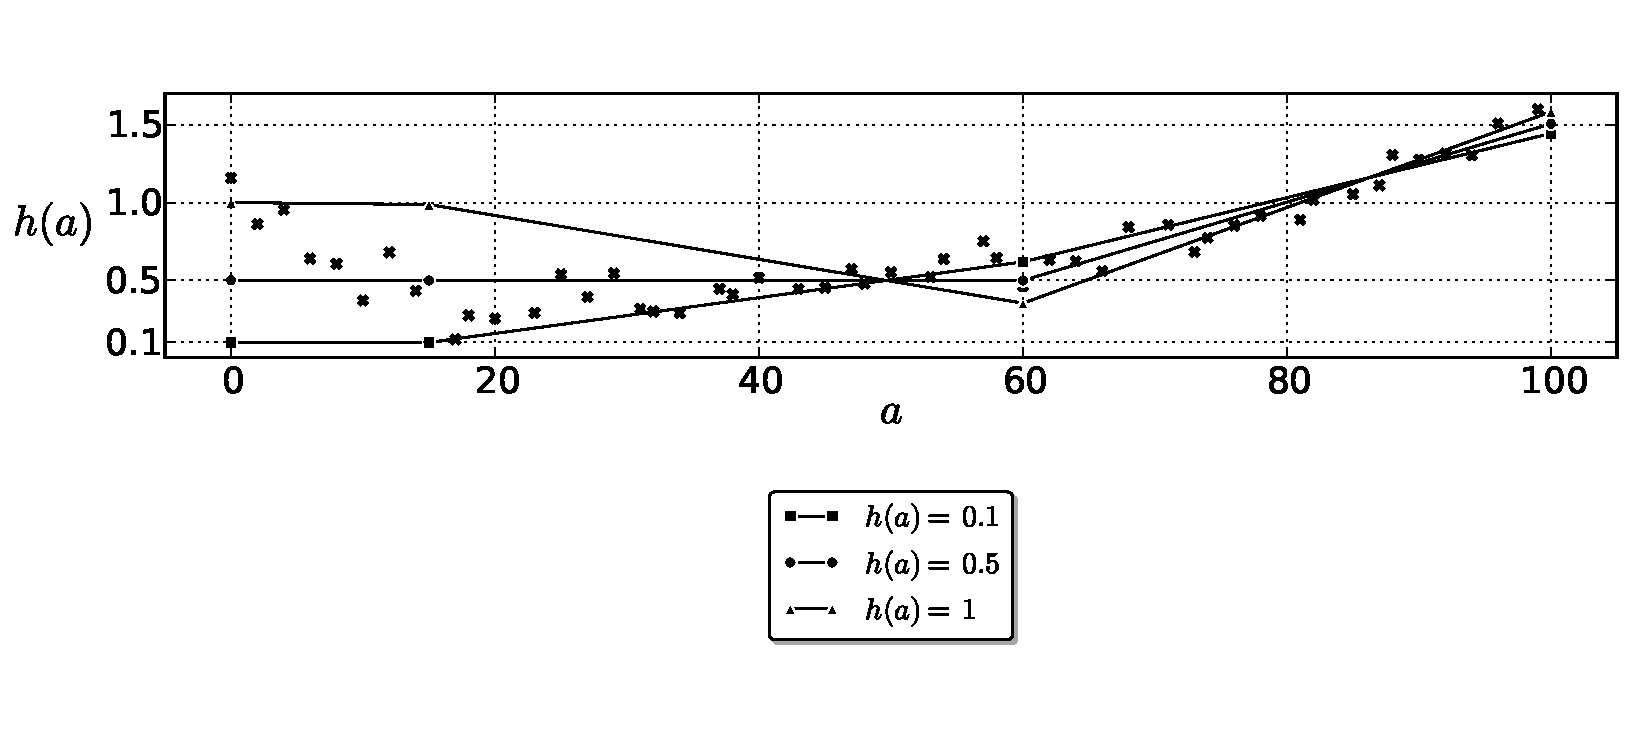
\includegraphics[width=\textwidth]{level_value-smoothing-splines.pdf}
\caption[An informative prior on the level of $h(a)$.]{An informative
  prior on the level of $h(a)$ for interval $0 \leq a <
  15$ changes the estimated rate dramatically for $a$ between $20$ and
  $60$ and even leads to different estimates for $a = 100$.  The more
  data available, the more knots in the model; the lesser the
  smoothing penalty, the less this level value assumption will affect
  the estimates for ages outside the interval, however.  }
\label{level-value-priors}
\end{center}
\end{figure}



These priors are implemented as ``hard-soft constraints.''  For a
value $v$ on age range $(a_0,a_1)$, the value of the spline model is
replaced with the level value for the age range (which I call a hard
constraint), and the prior density on the spline is augmented with a
penalty term for the offset log difference between the level value of
the unconstrained spline and $v$ (which I call a soft constraint). The
offset log difference penalty has the form
\[
\log\left(h(a)+\e)\right) \sim
 \Normal\left(\log\left(v + \e\right), \sigma^2\right),
\]
where $h(a)$ is the age-specific hazard function, $\e = 10^{-6}$ is the
offset to avoid taking the log of $0$, and $\sigma = 0.01$ is the
magnitude of the penalty.  In Bayesian terms, this encodes the belief
that the spline is expected to be within $1$\% of the expert level
value, provided the level value is not too close to $0$.

A similar sort of expert knowledge on the plausible bounds on
level is also useful, both in modeling noisy data and in increasing
the numerical stability of estimation algorithms. Again, however, the
implications of such a prior can be unexpected.
Figure~\ref{level-bounds-priors} shows the effects of three different
upper bounds on the spline estimation from the same data set as the
previous figure.

\begin{figure}[h]
\begin{center}
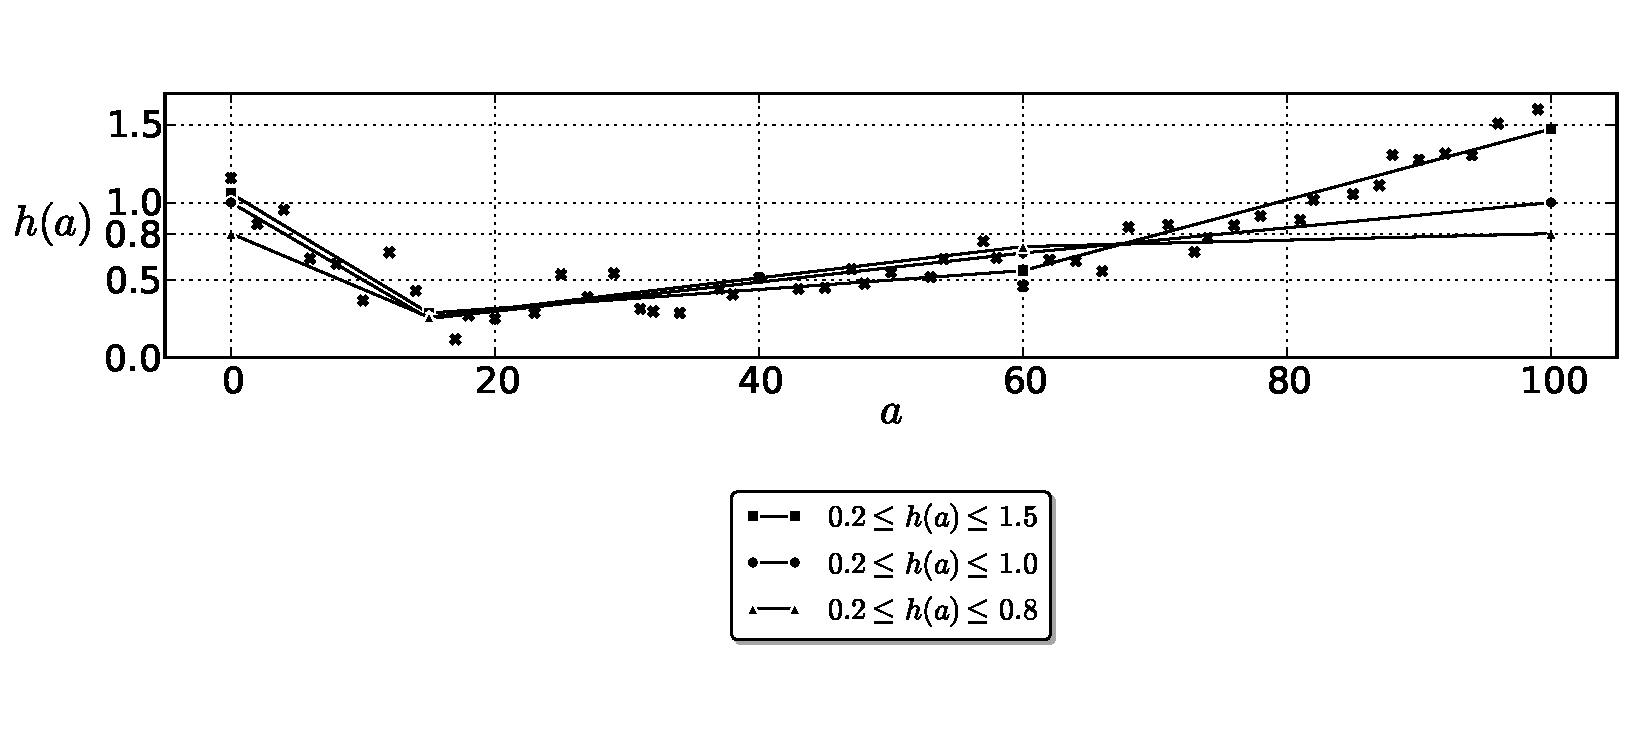
\includegraphics[width=\textwidth]{level_bound-smoothing-splines.pdf}
\caption[An informative prior on the upper and lower bounds of the
  age-specific hazard function $h(a)$.]{An informative prior on the
  upper and lower bounds of the age-specific hazard function $h(a)$
  changes the estimated hazard function dramatically for
  ages where the data are outside the bounds. For ages where the data
  are inside the bounds, the estimates are also affected, but to a lesser degree.}
\label{level-bounds-priors}
\end{center}
\end{figure}



Like the level value prior, this prior is also implemented as a
hard-soft constraint.  If the level bounds are $\ell_0 \leq h(a)
\leq \ell_1$, there is a hard constraint that replaces the spline with a
clipped version, $h^c(a) = \clip\left(h(a), \ell_0, \ell_1\right)$, and
also a soft constraint that ensures that the original spline is close to the clipped
spline in offset log-transformed space.

\section{Priors on monotonicity}

One common expert prior on age patterns is a strong belief that the
function is increasing or decreasing over a certain age
range. Mathematically speaking, these are priors on the sign of the
derivative of the age pattern.  For example, these priors can be implemented efficiently in
Bayesian Markov chain Monte Carlo (MCMC) computation by conditioning on the differences of the
age-specific hazard function $h(a)$:
\[
h(a) \geq h(a+1) \text{ for } a : a_s < a < a_e.
\]
The results of using such a prior are shown in
figure~\ref{monotone-age-pattern}.


\begin{figure}[h]
\begin{center}
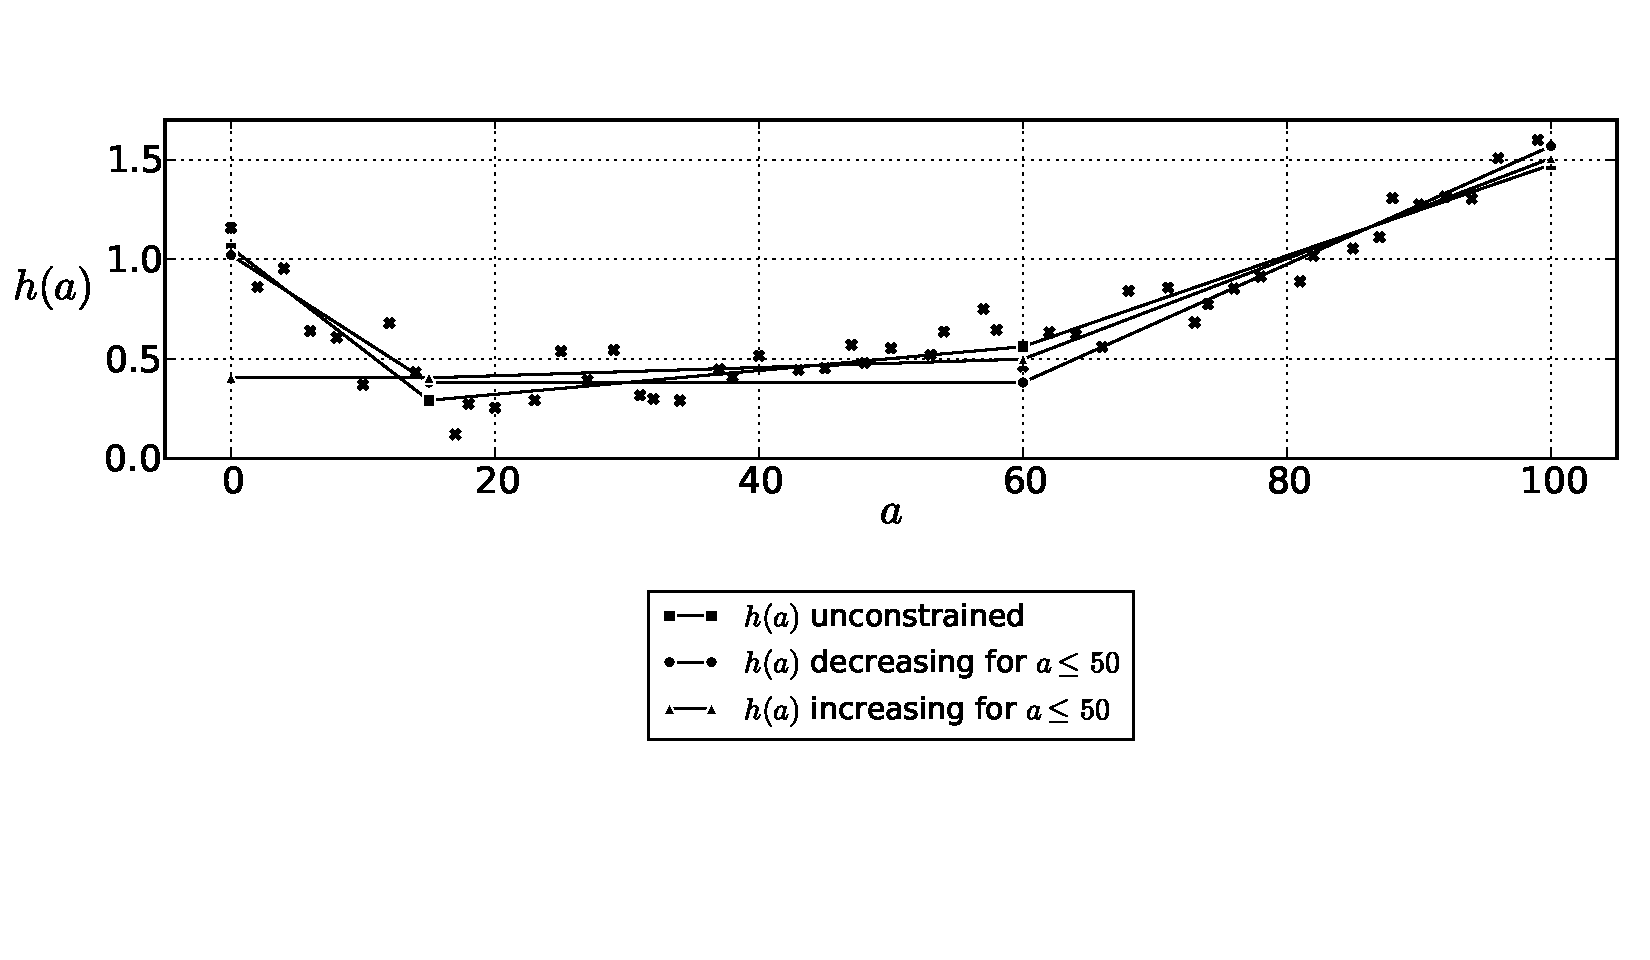
\includegraphics[width=\textwidth]{monotone-smoothing-splines.pdf}
\caption[An informative prior that the age pattern is increasing or
  decreasing across an age range.]{The expert belief that the age
  pattern is increasing or
  decreasing across an age range can also be implemented as a Bayesian
  prior.  When the prior is contrary to the data, the estimate will be
  as close to the data as possible while respecting the prior.  For
  example, the age-specific hazard function marked with triangles is the result
  of a prior belief that the age pattern increases from age $0$ to
  $50$ when confronted with data, shown as x-shaped marks that
  clearly decrease over this age range.}
\label{monotone-age-pattern}
\end{center}
\end{figure}


For computational efficiency, the increasing and decreasing
constraints are implemented as soft constraints.  For a constraint
that the function is decreasing between $a_s$ and $a_e$, I include the penalty
\[
\operatorname{clip}\left(\log h(a+1) - \log h(a), 0, 1\right) \sim \Normal(0, \epsilon^2)
\]
for a small value of $\epsilon$, like $\epsilon = 10^{-6}$.  This has
a fully Bayesian interpretation, encoding a belief that a decreasing age pattern is expected
and an increase of more than approximately $0.0003$\% is very surprising.


An area for future work comes from another common expert belief: that
the age pattern is unimodal.  This is conceptually clear, but
computationally it has proven more difficult to realize than
monotonicity.  While the monotonicity constraint maintains
log-concavity of the posterior distribution (if it was log-concave to
start with), a straightforward implementation of a unimodality
constraint will result in non-log-concave posterior distribution, even
if everything else is well behaved.  This suggests that the difficulty
in fitting such models is inherent in the local step method of the
MCMC algorithms I have been using.  Perhaps an alternative approach
such as the population Monte Carlo algorithm would be more successful.
Alternatively, there are some approximations of the unimodality
constraint that may be easier to optimize over.\cite{papp_shape_2012}

\section{Priors are not just for splines}
All three of the expert priors developed in this chapter are
applicable to any age-specific function derived from the compartmental
model in section~\ref{sys-dynamics}. Most importantly, the
age-specific prevalence $p(a) = C(a)/\left[S(a)+C(a)\right]$ can be augmented with expert
priors on level values (e.g., birth prevalence is $0$), level bounds
(e.g., no population has prevalence above $10$\%), and monotonicity
constraints (e.g., prevalence in increasing as a function of
age). Relative mortality risk $\frac{h_m(a)+h_f(a)}{h_m(a)}$ is another derived quantity
for which experts often have strong priors.

However, this sort of modeling requires care. The system dynamics
model enforces a precise consistency between the different
epidemiological rates, and making strong assumptions about one will
have implications for others.  Sometimes these implications are
counterintuitive.

As a practical matter, I recommend that modeling begin with as few
assumptions as possible to which expert priors may be added gradually. The
benefit of this is threefold.  First, fitting the model without all
the available expert knowledge allows the data to speak.  If the estimates
confirm the expert belief, that is reassuring, and if they show the
opposite, that is interesting. Second, the MCMC algorithm has a
pitfall: \emph{nonconvergence}. A quick way into this pit is
introducing inconsistent expert priors, for example, decreasing
prevalence and prevalence of $0$ at age $0$. By adding in expert
priors one at a time, the inconsistency that caused nonconvergence
will be more easily identified. Third, as with any model that produces
estimates from sparse and noisy data, it is essential to conduct a
sensitivity analysis to understand how influential modeling
assumptions are on the results.  The gradual addition of expert priors
will provide a starting point for this sensitivity analysis, showing
which expert priors are essential to obtaining reasonable results and
which are not as critical.

\section{Empirical priors on age patterns}
Another type of level prior worthy of separate exposition is that used
to implement the empirical Bayes approach that permits decomposing the
global estimation computation into region subcomputations that can be
run in parallel.  If estimates of the mean and standard deviation of
an age pattern are known for each age from a prior computation, this
information can be included in the age-specific hazard through a
penalty of the form
\[
h(a) \sim \Normal\left(\boldmu_{\text{prior}}(a),
\boldsigma_{\text{prior}}^2(a)\right).
\]

Since the model must cope with the order-of-magnitude differences of age-specific rates, it can be more robust to use an empirical prior relating the offset log-transformed rates:
\[
\log\left(h(a)+\epsilon\right) \sim \Normal\left(\log\left(\boldmu_{\text{prior}}(a)+\epsilon\right),
\left(\frac{\boldsigma_{\text{prior}}+\epsilon}{\boldmu_{\text{prior}}+\epsilon}\right)^2\right).
\]

\section{Statistical Models for Epidemiological Rates}
\label{theory-rate_model}

The key to connecting the systems dynamics model from
Chapter~\ref{theory-system_dynamics} to the evidence base collected
through systematic review is the \emph{rate model}.  This is a
statistical model, which has its core features defined by its
likelihood function.  By \emph{likelihood function}, I mean a
probability density function that assigns a value for the likelihood
of every possible (rate value, uncertainty)-pair for each setting of
the model parameter.  An examples will make this clearer, so I turn
now to the meta-analysis of population prevalence of schizophrenia in
adult males.  The forest plot in
Figure~\ref{fig:theory-rate_model-schiz_forest} shows the results of
combining $<<len(d['schiz_forest.json|dexy']['r'])>>$ studies using
$7$ different rate models.  As the figure demonstrates, the choice of
rate model can have a huge effect on the estimated uncertainty, and
can have a noticable effect on the estimated median as well. The
models I displayed produce point estimates ranging from
$<<d['schiz_forest.json|dexy']['min_est']>>$ to
$<<d['schiz_forest.json|dexy']['max_est']>>$, and uncertainty
intervals with widths ranging from
$<<d['schiz_forest.json|dexy']['min_spread']>>$ to
$<<d['schiz_forest.json|dexy']['max_spread']>>$.

In what follows, I will develop a collection of rate models, starting
with the simplest and then increasing complexity, while identifying
the benefits and drawbacks of each.  The models to come, in order, are
the binomial model, the beta-binomial model, the poisson model, the
negative binomial model, and three variants of the normal
model.

\begin{figure}
\begin{center}
\includegraphics[width=\textwidth]{theory-rate_model-schiz_forest_plot.png}
\end{center}
\caption{Forest plot summarizing $7$ alternative models for
  meta-analysis of adult male schizophrenia prevalence at
  population-level.  The median estimates range from
  $<<d['schiz_forest.json|dexy']['min_est']>>$ to
  $<<d['schiz_forest.json|dexy']['max_est']>>$, and the width of the
  $95\%$ HPD interval ranges from
  $<<d['schiz_forest.json|dexy']['min_spread']>>$ to
  $<<d['schiz_forest.json|dexy']['max_spread']>>$.}
\label{fig:theory-rate_model-schiz_forest}
\end{figure}

\subsection{Binomial Model}
My conceptually simplest model for rate data was built from the
binomial random variable, which follows the probability distribution
\[
\Pr[X=k\given n,\pi] = \binom{n}{k}\pi^n(1-\pi)^{n-k}
\]
I've used greek to emphasize that $\pi$ is the parameter, while $n$
and $k$ are data.

Although this equation may appear opaque, the intuition behind it is
simple: $n$ individuals were tested for a disease, and $k$ tested
positive. The formula then follows from the assumption that each
individual tested positive with probability $\pi$, and that 
knowing about the test results of any subset of individuals gives me
no information about what the test results the others were
(these events are ``independent'').

This distribution inspires a computationally tractable and
theoretically appealing rate model for a observed population rate of
$r$ from a population of size $n$:
\[
\dens(p,n\given \pi) \propto \pi^{\lfloor rn \rfloor}(1-\pi)^{\lceil (1-r)n \rceil}.
\]
Note that it is not necessary to include the term $\binom{n}{nr}$,
because this does not depend on the model parameter $\pi$. There is a
constant of proportionality, which is necessary to make this rate
model truely a probability density function for any $\pi$, but happily
I will never need to know this constant, and I have use the ``proportional to''
symbol $\propto$ instead of equality to emphsize this fact.

The funnel plot in Figure~\ref{fig:theory-rate_model-binom_funnel}
shows the predictive distribution of this rate model for $\pi=<<
d['binomial_model.json|dexy']['pi_binomial_funnel'] >>$.  It also shows
the potential problem with this approach: the data gathered by
systematic review are often much more dispersed than this
distribution predicts.

\begin{figure}[ht]
\begin{center}
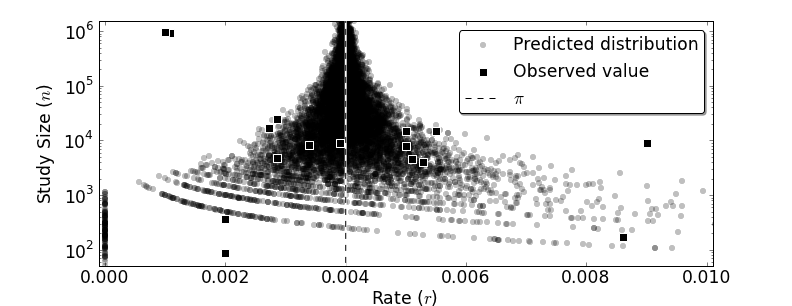
\includegraphics[width=\textwidth]{binomial-model-funnel.png}
\end{center}
\caption{Funnel plot showing predictive distribution for the binomial
  rate model with
  $\pi=<<d['binomial_model.json|dexy']['pi_binomial_funnel']>>$ (shown in
  blue), with data from systematic review for adult male schizophrenia
  prelvanece overlaid for comparison (shown in green).}
\label{fig:theory-rate_model-binom_funnel}
\end{figure}

All models are wrong, of course, so why does this model require
refinement? The answer is that is leads to unreasonably high
confidence when modeling noisy data.  If a study of
$<<d['binomial_model.json|dexy']['pop_A_N']>>$ people from in
subpopulation A finds prevalence of
$<<d['binomial_model.json|dexy']['pop_A_prev']*1000>>$ per thousand and
a study of $<<d['binomial_model.json|dexy']['pop_B_N']>>$ people in
subpopulation B finds $<<
d['binomial_model.json|dexy']['pop_B_prev']*1000 >>$, then the
binomial model predicts that a study of
$<<d['binomial_model.json|dexy']['pop_C_N']>>$ people in subpopulation
C will have prevalence of
$<<d['binomial_model.json|dexy']['pop_C_prev_per_1000']>>$, with
$95\%$ HPD interval
$<<d['binomial_model.json|dexy']['pop_C_ui_per_1000']>>$.  I have
no problem with the point estimate.  Picking the mean of the two
populations seems just right.  But the uncertainty interval lacks face
validity.  It would be much more reasonable to have an uncertainty
interval as large as $[1,7]$, instead of one as small as this.

One way to formalize this objection is through the posterior
predictive check, an in-sample goodness-of-fit test that can be done
graphically.  Figure~\ref{fig:theory-rate_model-binom_ppc} shows the
posterior predictions of the binomial model when it is fit to the
adult male schizophrenia dataset, together with the data itself.  The
model predictions are clearly compressed, and trusting the results of
such a model will lead to inappropriate certainty in the face of noisy
data.

\begin{figure}[ht]
\begin{center}
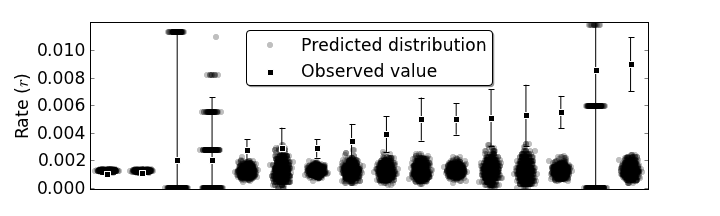
\includegraphics[width=\textwidth]{binomial-model-ppc.png}
\end{center}
\caption{Posterior predictive check for binomial model fit to adult
  male schizophrenia data.  Blue shows 1000 draws from the posterior
  distribution of the binomial model, and green shows the input data.}
\label{fig:theory-rate_model-binom_ppc}
\end{figure}




\subsection{Beta-binomial model}
A theoretically appealing extension to the binomial model (which also
does not work for my purposes) is the beta-binomial model.  I will
develop it in this section, to motivate the following sections.

Formally, the beta binomial random variable is given by the following
probability distribution
\begin{align*}
\Pr[X = k\given n, \alpha, \beta] 
  &= \int_{\pi}\dens(\pi\given \alpha, \beta) \binom{n}{k}\pi^k(1-\pi)^{n-k}
d\pi\\
\dens(\pi\given \alpha, \beta) &\propto \pi^{\alpha-1}(1-\pi)^{\beta-1}
\end{align*}

The intuition behind this model is simpler than the equation, however.
As in the binomial model, each individual tests positive for the condition independently
with a probability $\pi$, but now $\pi$ itself is a random variable,
distributed according to a beta distribution with parameters $\alpha$
and $\beta$. The beta distribution is given by 
\[
\dens(\pi\given \alpha, \beta) =
\frac{\Gamma(\alpha+\beta)}{\Gamma(\alpha)\Gamma(\beta)}\pi^{\alpha-1}(1-\pi)^{\beta-1}
\]
and has a high degree of flexibility.  It also always takes values
between zero and one, making it an appropriate distribution for a
probability.  Figure~\ref{fig:theory-rate_model-beta} shows the
probability density of the beta distribution for several combinations
of $\alpha$ and $\beta$.
\begin{figure}[ht]
\begin{center}
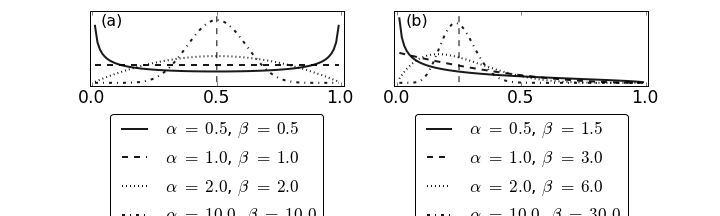
\includegraphics[width=\textwidth]{beta-distribution.png}
\end{center}
\caption{Probability density for the beta distribution for a range of
  $\alpha$ and $\beta$ values. Dashed black line shows expected value,
which is $.5$ for all distribution in a) and $.25$ for all in b).}
\label{fig:theory-rate_model-beta}
\end{figure}

The beta binomial distribution inspired the following rate model for
an observed population rate of $r$ from a population of size $n$:
\[
\dens(r,n\given \alpha, \beta) \propto \int_{\pi}
\pi^{\alpha-1}(1-\pi)^{\beta-1} \pi^{\lfloor rn\rfloor} (1-\pi)^{\lceil (1-r)n\rceil}
d\pi.
\]

This model extends the binomial model in a way analogous to how a
random effects model in linear regression.  By introducing an
additional dimension in to the parameter space, it is able to capture
the dispersion beyond the binomial model that I have observed
empirically in funnel plots of real data
(Figure~\ref{fig:theory-rate_beta-binomial-funnel} shows the beta
binomial funnel plot, as well as the posterior predictive check for
this model on the same data as used in
Figure~\ref{fig:theory-rate_model-binom_ppc}.

\begin{figure}[ht]
\begin{center}
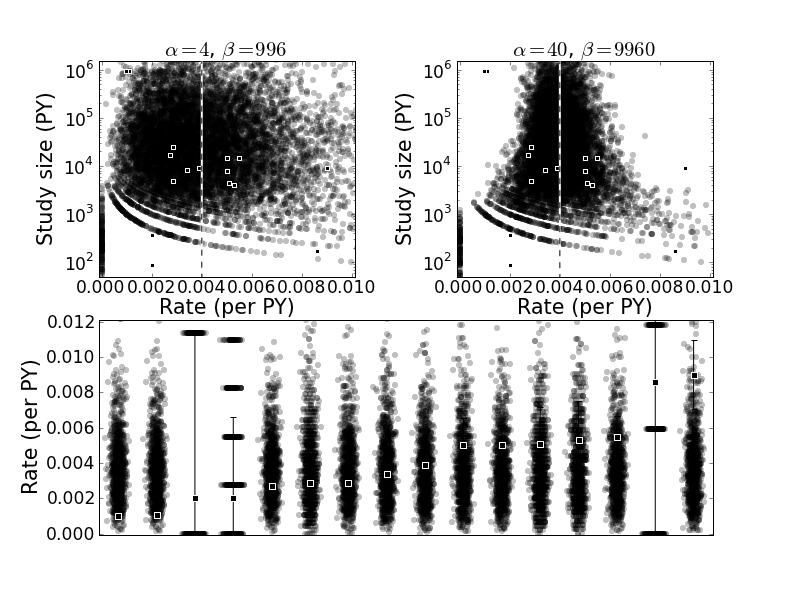
\includegraphics[width=\textwidth]{beta-binomial-funnel.png}
\end{center}
\caption{Funnel plot and posterior predictive check for beta binomial model.}
\label{fig:theory-rate_beta-binomial-funnel}
\end{figure}

This model addresses the theoretical shortcoming raised in the
previous section: if studies of
$<<d['beta_binomial_model.json|dexy']['pop_A_N']>>$ people show prevalences
of $<<d['beta_binomial_model.json|dexy']['pop_A_prev']*1000>>$ and
$<<d['beta_binomial_model.json|dexy']['pop_B_prev']*1000>>$ per thousand,
then the posterior distribution of the beta binomial model has mean
$<<d['beta_binomial_model.json|dexy']['pop_C_prev_per_1000']>>$ with 95\%
HPD interval $<<d['beta_binomial_model.json|dexy']['pop_C_ui_per_1000']>>$,
which seems quite reasonable.

The great shortcoming of the beta binomial model is computational.  As
will be elaborated in Chapter~\ref{theory-numerical_algorithms}, there
is no closed-form solution to the integral in the probability density
for the beta binomial model.  Evaluating it requires introducing a
latent variable for each of the data points in the likelihood.  This
simply had too much cost for the numerical algorithms and
computational infrastructure available.  So my search
continued.

\subsection{Other count models}
There are two traditional approximations to the binomial distribution,
depending on how large $k$ is in relation to $n$.  When $k/n$ is
large, the normal distribution is used, and when $k/n$ is small, the
binomial is similar to the Poisson distribution.

Since I expect to usually be in a ``small $k/n$'' setting, I will not
develop the normal model in detail now, although in the next section I
will develop to model based on monotonic transformations of the normal
distribution which include a normal model as a special case.

The Poisson distribution is given by the the equation
\[
\Pr[X=k] = \frac{\lambda^k e^{-\lambda}}{k!},
\]
and it can be understood intuitively as the number of times a
``memoryless'' event occurs in a unit time period.  Setting $\lambda =
\pi n$ produces an approximation to the binomial distribution, which
is quite accurate for large $n$ and small $k$.
Figure~\ref{fig:theory-rate_model-poisson_approx_to_binom}
demonstrates how precise this approximation can be when approximating
a binomial distribution with
$n=<<d['poisson_model.json|dexy']['n_small']>>$ and
$\pi=<<d['poisson_model.json|dexy']['pi_true']>>$.

\begin{figure}
\begin{center}
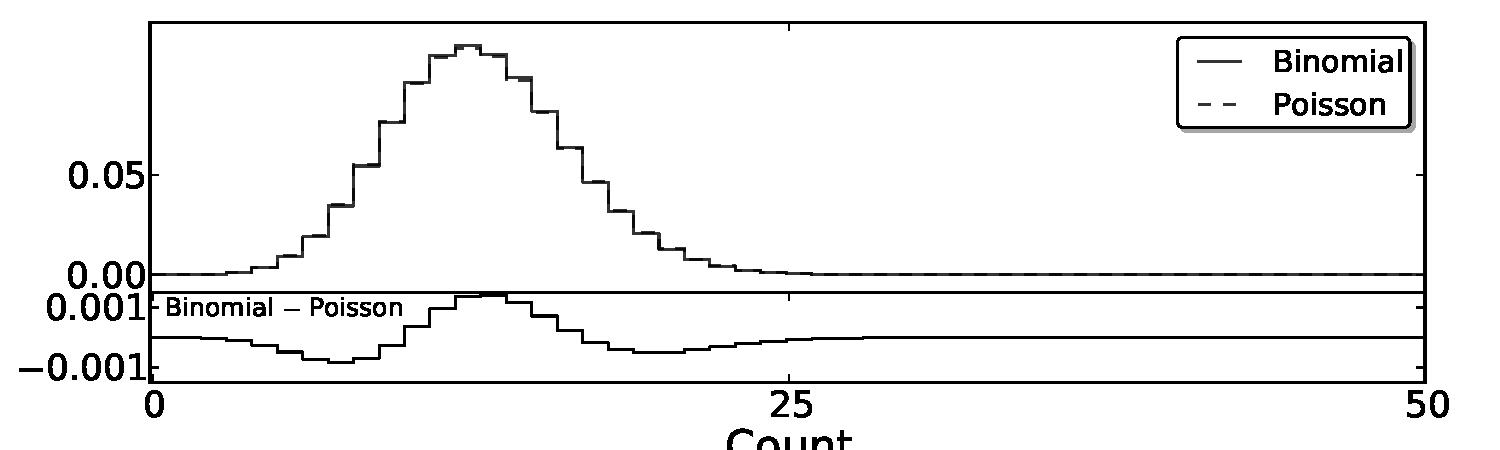
\includegraphics[width=\textwidth]{poisson_approx_to_binom.png}
\end{center}
\caption{The Poisson distribution approximates the binomial
  distribution very closely. Here a binomial distribution with
  $n=<<d['poisson_model.json|dexy']['n_small']>>$ and
  $\pi=<<d['poisson_model.json|dexy']['pi_true']>>$ is approximated by
  a Poisson distribution with parameter
  $\lambda=<<d['poisson_model.json|dexy']['n_small'] *
  d['poisson_model.json|dexy']['pi_true']>>$.  The difference between
  the distributions is shown in the lower panel, since the curves in
  the upper panel are almost indistinguishable by eye.}
\label{fig:theory-rate_model-poisson_approx_to_binom}
\end{figure}

Because of the similarity of these distributions, the Poisson model,
is defined by
\[
\dens(r,n\given \pi) \propto (\pi n)^{\lfloor rn\rfloor} e^{-\pi n}.
\]
It is subject to all of the concerns raised about the
binomial model regarding inappropriately low levels of uncertainty
when modeling rates with non-sampling variation at the level typically
gathered in systematic review.

There is one key benefit to this model, compared to the binomial and
beta-binomial models, however.  The Poisson model assigns a
theoretically justified and non-zero likelihood to rates of more than
one.  Although prevalence is always less than one, it is theoretically
possible to have incidence rates more than one, and remission rates
are often more than one (per person-year).

Another benefit from this approach is to be found in its
over-dispersed variant.  This distribution
is called the negative binomial distribution (named after the formula
that the proves it does indeed sum to one).  Unlike the beta-binomial
distribution, it \emph{does} have a closed form (if you consider the gamma function ``closed''):
\[
\Pr[X = k\given \pi, \delta] = \frac{\Gamma(k+\delta)}{\Gamma(\delta)k!}
\left(\frac{\delta}{\pi+\delta}\right)^\delta \left(\frac{\pi}{\pi+\delta}\right)^k
\]

However, this closed form obscures the intuition behind the negative
binomial distribution, which is quite similar to the intuition behind
the beta-binomial distribution, although less clear from the
name. Through a bit of algebra, the negative binomial distribution can
be represented as a hierarchical model, where the observed data comes
from a Poisson distribution, and the parameter of the Poisson
distribution is itself a random variable that comes from a gamma
distribution:
\begin{align*}
X\given \pi &\sim \Poisson(\pi)\\
\pi &\sim \GammaDist(\mu, \delta)
\end{align*}
Here the Gamma distribution is defined by (TK reparameterize to match above)
\[
\dens(x; k,\theta) =
x^{k-1} \frac{e^{-x/\theta}}{\theta^k \, \Gamma(k)}.
\]
Through this lens, the negative binomial model can be interpreted as a
nature adaptation of the traditional random effects model in linear
regression to the Poisson case, where each observation comes from a
different Poisson model and the Poisson parameter of these models are
all drawn from a common Gamma distribution.

Thus a rate model based on it provides benefits in handling
non-sampling variation similar to those demonstrated for the beta
binomial distribution above, but in a formulation that is much less
demanding computationally.  The negative-binomial rate model for
observing a rate of $r$ in a population of size $n$ is:
\[
\dens(r,n\given \pi, \rho) \propto \frac{\Gamma(\lfloor rn\rfloor+\rho)}{\Gamma(\rho)} (1-\pi)^\rho \pi^{rn}.
\]

A difficultly I have observed in practice with the negative binomial
model is in the realm of numerical algorithms.  My experience has been that these
likelihoods lead to models that are simply harder to fit than
traditional normal models.  Nonetheless, the negative binomial model
has been the primary tool in the likelihod modeling for the
applications to be presented in Chapters~\ref{practice-all-examples}.

Chapter~\ref{TK} will examine the properties of numerical algorithms
for fitting the negative binomial model in more detail, but one
approach which has helped substantially is imposing an informative
prior on the over-dispersion parameter of the negative binomial
distribution.  Because it seems unreasonable to impose a very
informative prior on the over-dispersion parameter, I have limited the
possibilities to augmenting the hierarchical formulation of the
negative binomial model above with the following:
\[
\log_{10} (\delta-5) \sim \Normal\left(\mu_{\log\delta}, .25^2\right),
\]
with $\mu_{\log\delta} = 1, 2, 3$.  The results of adding this
prior are contrasted with the results vanilla negative binomial model
(with an uninformative prior on $\delta$) in
Figure~\ref{fig:theory-rate_model-neg_binom_priors}, which shows that
a belief a priori that the observations is more over-dispersed leads
to a posterior estimate where the predicted rate have more
uncertainty, as expected.

\begin{figure}
\begin{center}
\includegraphics[width=\textwidth]{neg_binom_priors.png}
\end{center}
\caption{Forest plot of a simulation experiment demonstrating the
  effect of a weakly informative prior on the negative binomial model
  posterior.  Sixteen data points simulated from a negative binomial
  distribution are fit with negative binomial models, with $5$
  different priors on the dispersion term $\delta$.  The informative
  prior of $\delta = \infty$ reduces the negative binomial model to
  the poisson model, and for this case the uncertainty interval does
  not contain the truth.  All of the weakly informative priors do
  contain the truth, however.  Replicating this simulation
  $<<d['neg_binom_sim.json|dexy']['replicates']>>$ times yielded mean
  bias of
  $\E[\pi_{\true}-\pi_{\median}]=<<d['neg_binom_sim.json|dexy']['bias']['pi']>>$
  and root mean squared error of
  $\RMSE[\pi_{\true}-\pi_{\median}]=<<d['neg_binom_sim.json|dexy']['rmse']['pi']>>$;
  the uncertainty interval contained the $\pi_{\true}$ value with probability
  $<<d['neg_binom_sim.json|dexy']['percent_coverage']['pi']>>$.}
\label{fig:theory-rate_model-neg_binom_priors}
\end{figure}

\subsection{Transformed normal models}
Some epidemiological data is not count data at all.  Duration studies
and studies measuring the relative risk of mortality are two that come
up frequently in systematic review.  For duation data, a normal model
has been quite sufficient, and a log-normal model has proven
appropriate for modeling relative risk data, which can be thought of
as a ratio of count variables.

Transformed normal models have also been used for mortality rates in
the past [ref including GK TK], and are worthy of continued consideration for
modeling the incidence, prevalence, remission, and mortality as an
alternative to the negative binomial.

In this section, I will develop a general transformed normal model,
and compare it to the negative binomial model.  The adjective
``transformed'' refers to a function which I will keep quite general
for now, requiring it only to be increasing and differentiable,
i.e. for any $x > y$ the transformation $f$ must have $f(x) > f(y)$
and $f'(x)$ must be defined.  Then transformed normal model will be
derived from the normal distribution, defined by the probability
density
\[
\dens(x\given \pi, \sigma) \propto \frac{1}{\sigma} \exp\left\{ -\frac{(x-\pi)^2}{2\sigma^2} \right\}.
\]

For any increasing, differentiable function $f$, this distribution can be converted to
an $f$-transformed normal model with probability density
\[
\dens(r,s\given \pi, \sigma, f) \propto \exp\left\{-\frac{\left(f(r)-f(\pi)\right)^2}{2\left((sf'(r))^2+\sigma^2\right)}\right\},
\]
where $s$ is the standard error of the rate $r$, which is more
convenient that the effective sample size $n$ in this case. The
denominator of the exponent deserves some additional discussion.  For
the identity function $f(x) = x$, the derivative $f'(x) = 1$, and the
denominator simplifies to $2(s^2 + \sigma^2)$, a familiar ``inverse
variance'' weighting where $\sigma$ is a random effect to account for
over-dispersion.  When $f$ is a more complicated function, the term
$sf'(r)$ approximates the standard error of the transformed value
$f(r)$.  Although more sophisticated approximations are possible,
experience dictates that the non-sampling variation (parameterized by
$\sigma$) is always larger than the chance variation, so a simple
approximation of the chance variation is sufficient.

Some common transformations $f$ used in related work yield the
lognormal model ($f(x) = \log x$) the logit model ($f(x) = \logit x$)
and the probit model ($f(x) = \probit x$).  All of these approaches
have a significant drawback, however.  The transform is not defined
for $x=0$, so these models cannot use data showing rates of zero.
There are two common methods to fix this, dropping all zeros, and
adding a small offset.  Dropping measurements of zero is clearly
problematic, as it leads to systematic bias in the data that remains
and produces estimates larger than they should be.  This is especially
true for high quality studies which focus on the age pattern of a
disease, where it is quite reasonable for some age groups to have zero
cases observed.  The effect of dropping zeros is to overestimate the
rates in these age groups.

Adding a small amount, such as $0.5$ is an alternative solution, and
indeed, this is the approach taken for cause-specific mortality estimation
in GK [ref TK].  The selection of the offset can appear ad hoc,
however.

Within the framework of the transformed normal model, there is
room to put the solution on firm theoretical foundations.  For
example, by taking $f_\zeta(x) = \log(x + \zeta)$, I obtained the
``offset log transformed model'', which does allow rates of zero,
simply by taking a positive value for $\zeta$.  This model will not be
used extensively in the example application to come later in this
book, but it seems like a promising approach.  It is particularly
appealing in the way it decomposes the non-sampling variation into an
additive error $\zeta$ and a multiplicative error $\sigma$, and I
expect that it will prove useful in the future.  For completeness,
here is the probability density for the offset log transformed model:
\[
\dens(r,s\given \pi, \sigma, \zeta) \propto
\exp\left\{-\frac{\left(\log(r+\zeta)-\log(\pi+\zeta)\right)^2}{2\left(\left(\frac{s}{r+\zeta}\right)^2+\sigma^2\right)}\right\}.
\]

\subsection{Lower-bound data model}
Cause-specific mortality rates are a special case among the
epidemiological rates available for integrative systems modeling of
disease in a population.  These data come from carefully processing of
vital registration system output, from verbal autopsy stdies, and from
some other sources. But unlike incidence, prevalence, and remission
data, there is no rate or ratio in the compartmental model that
corresponds directly to this quanbtity.  This is because of the ``one
death has one cause'' mantra of biomedical theory.  The excess
mortality rate in the system dynamics model from Chapter TK is not
entirely compatible with this idea.

Cause-specific mortality data nonetheless provides \emph{some}
information, and should be used in an integative model if it is
available, especially if other sources are sparse and noisy (they
always are, in my experience).  By decomposing the excess mortality
into part that is ``cause-of-death mortality'' and residual excess
mortality, i.e. $f = f_{cod} + f_{non}$, it follows that $CSMR =p
\cdot f_{cod} \leq p\cdot f$, so the following lower bound model is
appropriate:
\[
\dens(CSMR \given \pi,\delta)
=
\begin{cases}
\calD(CSMR, \pi, \delta), &\qquad\text{if } \pi-CSMR \geq 0;\\
\calD(\pi, \pi, \delta), &\qquad\text{otherwise.}
\end{cases}
\]

\subsection{Summary and Comparison}
This section has developed $7$ alternative rate models, all with
benefits and drawbacks.  The binomial model is simple and
theoretically appealing, but does not handle non-sampling variation,
producing over-confident estimates in the face of noisy data.  The
beta binomial model deals with over-dispersion through a theoretically
appealing extension to the binomial model, but it is too
computationally demanding to use in my applications.  The poisson
model is a close approximation to the binomial model, and has all of
the drawbacks except it can handle rates greater than 1, which is
important for modeling remission rates.  So it is the negative
binomial model, which extends the poisson model analogously to the way
the beta binomial model extends the binomial model that I have settled
on for most of the applications to follow, using it to model
incidence, prevalence, remission, excess-mortality, and cause-specific
mortality. It is not as ammenable to analysis as I would like however,
and sometimes benefits from weakly informative priors on the
over-dispersion parameter, an undesirable feature that slows down
analysis by requiring sensitivity analysis.  Transformed normal models
are a promising alternative approach, and I have used the normal model
for duration data in some of the following examples, as well as
the lognormal model for standardized mortality rate data and relative
mortality risk data. The offset log transformed model seems
particularly promising as an alternative to the negative binomial
model, and understanding its statistical and computational
characteristics is a promising direction for future research.

TK some sort of comparison: simulation study? posterior predictive
checks? something analogous to SMART counties in small areas
estimation?

\chapter{Statistical models for heterogeneous age groups}
\chapterprecis{Abraham D. Flaxman}
With a full development of statistical rate models for a single age
group behind us, and the mathematical model for an age-specific rate
function laid out as well, this section turns to a peculiar feature of
population rate metaregression: the wide variety of age groups reported
in the literature.

A typical example of the heterogeneity in age groups is shown in for
the systematic review results on atrial fibrilation (AF)
prevalence\cite{TK_AF_report_reference} in
Figure~\ref{age-group-model-af-age-groups}.  The midpoint of the age
group is scattered against the width of the age group.  Simply put,
there is no standard set of age groups for AF research, and different
studies report results with different age groups. Unfortunately, this
phenomenon is far from unique to AF.

\begin{figure}[h]
\begin{center}
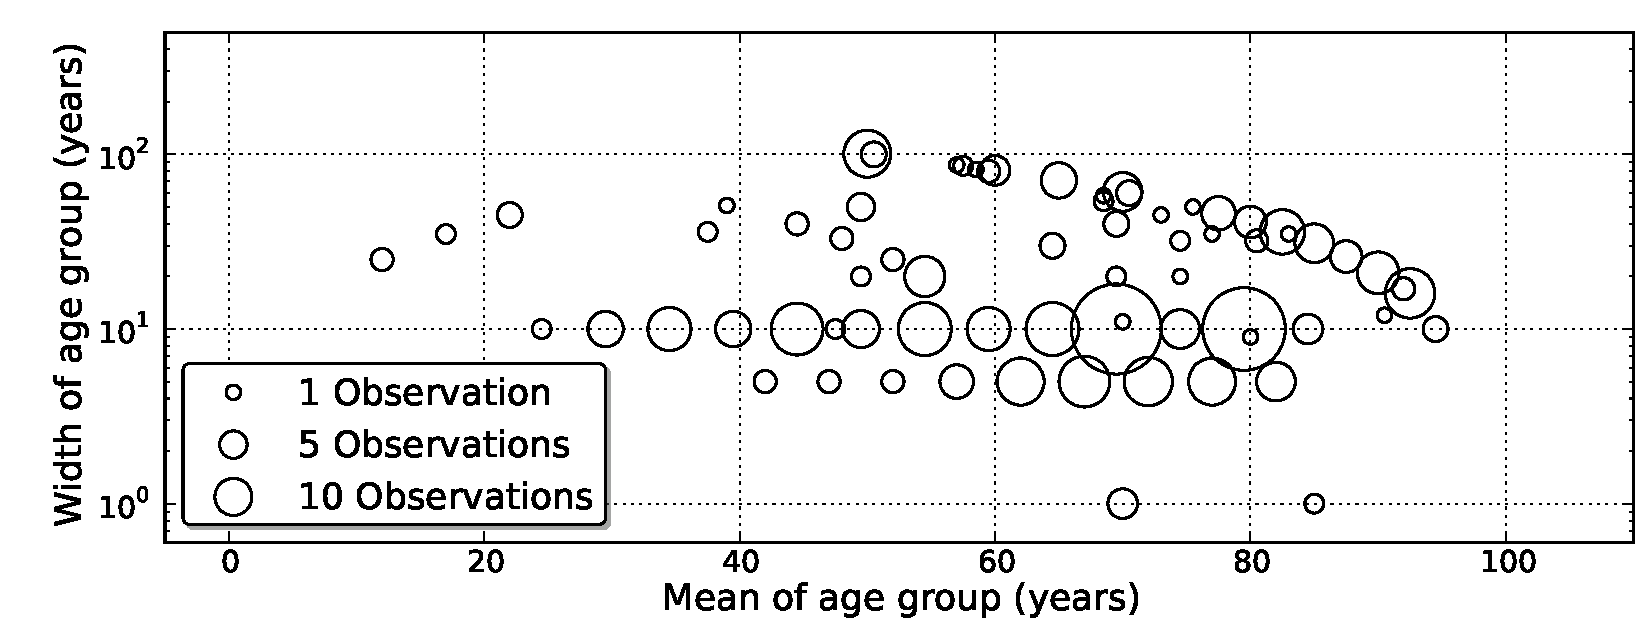
\includegraphics[width=\textwidth]{af_age_groups_scatter.pdf}
%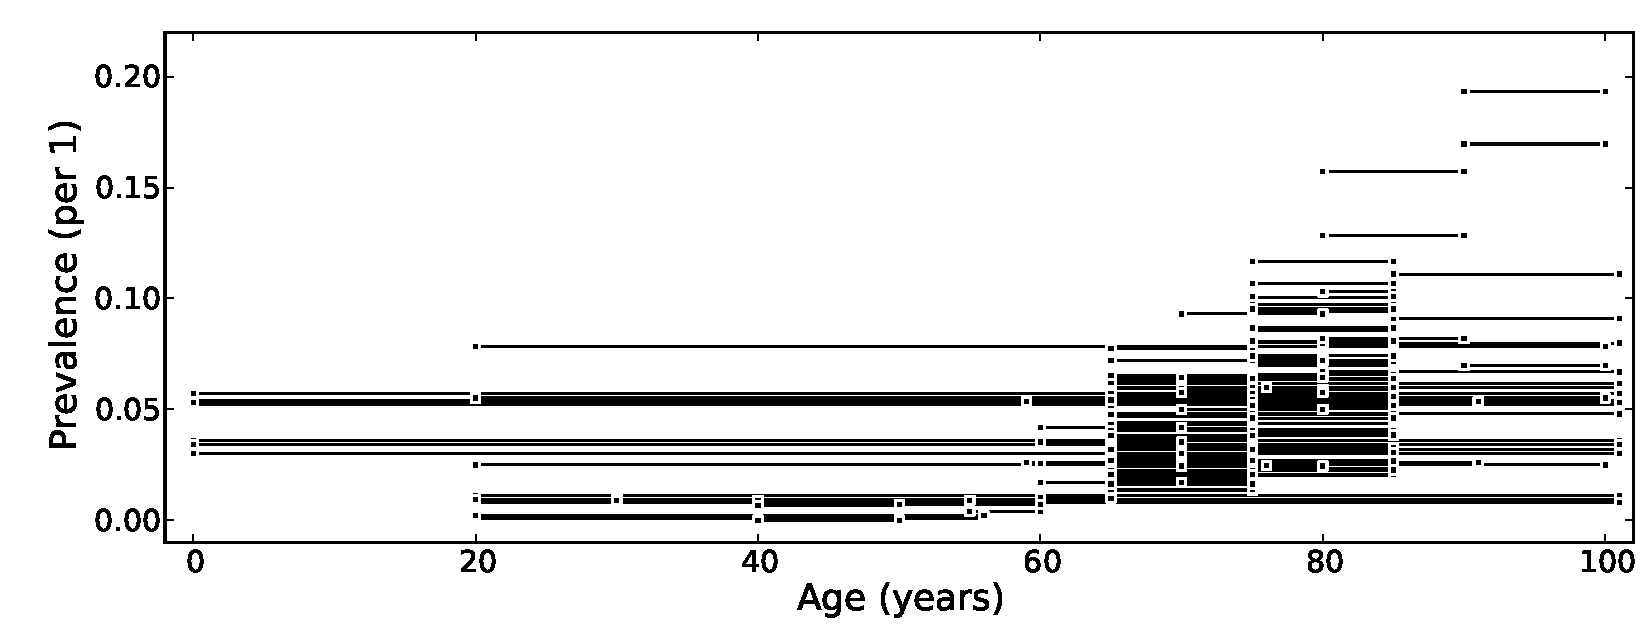
\includegraphics[width=\textwidth]{af_ages_intervals.pdf}
\end{center}
\caption{Mean and spread of age groups in the prevalence data
  collected from a systematic review of atrial fibrilation. The
  size of the circle shows how many observations of this age group
  were found in systematic review. There were
  $586$ rows of prevalence data
  extracted, but the most common age group accounted for only
  $68$ rows.}
\label{age-group-model-af-age-groups}
\end{figure}

This variation in reporting would not be problematic if I had access
to the microdata from all of the systematic review studies.  For
example, using microdata from a national health information system or
from a demographic household survey, I could simply tally the
prevalence rates by single-year age groups.  Although each individual
rate gathered in this way would have high variability, the rate model
from Chapter~\ref{theory-rate_model} combined with the spline model
for an age-specific hazard function from Chapter~\ref{theory-age_pattern_model} would
work together to produce an estimate that is as uncertain as it should be.

Re-analysis from microdata is occasionally implemented in a GBD study,
however it is often not an option.  I expect the use of microdata
re-analysis to become more frequent in national and subnational
settings.  In the more common situation where rate microdata are not
available, the rates cannot be retallied into homogeneous age groups,
and an alternative approach is needed.

There are several statistical approaches which I have considered, and
they will be compared and contrasted in this section.  Before getting
into the details, however, it is worthwhile to examine theoretically
the way that age grouping functions.

I begin with a simple mechanistic model of the age grouping process.
A study conducts some sort of measurement on a population of
individuals who are all of different ages and then the
epidemiological rate or rates of interest are tallied for age groups
selected in some context dependent manner. If the study was a
prevalence study using a full census sample, for example, and if I use
$r_{a_0,a_1}$ to denote the rate for age group $(a_0, a_1)$ and
$n_{a_0,a_1}$ to denote the subpopulation size of age group
$(a_0,a_1)$, then the identity
\[
n_{a_0, a_2} = n_{a_0,a_1} + n_{a_1,a_2}
\]
says nothing more complicated than that the size of the subpopulation
of age at least $a_0$ and less than $a_2$ is the sum of the size of
the subpopulation between age $a_0$ and $a_1$ and the size of the
subpopulation between age $a_1$ and $a_2$.  Applying the same
observation to the part of these subpopulations that have the condition
of interest yields the following identity:
\[
r_{a_0,a_2} = r_{a_0,a_1}\frac{n_{a_0,a_1}}{n_{a_0,a_2}} + r_{a_1,a_2}\frac{n_{a_1,a_2}}{n_{a_0,a_2}}. 
\] 
In a limiting case of a very large population with very fine age
intervals, this becomes:
\[
r_{a_0,a_2} = \int_{a=a_0}^{a_2} r_{a,a+\d a}\frac{n_{a,a+\d a}}{n_{a_0,a_2}}\d a.
\]
Undoubtedly all real studies are more complicated than this full
census of prevalence, but this is a starting point for conceptualizing
where age-grouped rates come from.  Roughly, they are integrals over
instantaneous rates for infinitesimal age groups.

\section{Overlapping age group data}
\label{theory-age_group_model-overlapping_data}
This section explores an examples of overlapping age group data
collected in systematic review through graphical statistics.  The
primary way I like to display overlapping age group data is shown in
Figure~\ref{theory-age_group_model-dismod_data_plot} as horizontal
lines on a plot of age versus rate value.  The level of the bars shows
the rate value, while the width of the bars shows the range of ages
included in the age group. It is often informative to augment these
lines with error bars, showing the uncertainty reported for each rate
value, but for this section I have left out the representation of
uncertainty to keep the plots as simple as possible.

\begin{figure}[ht]
\begin{center}
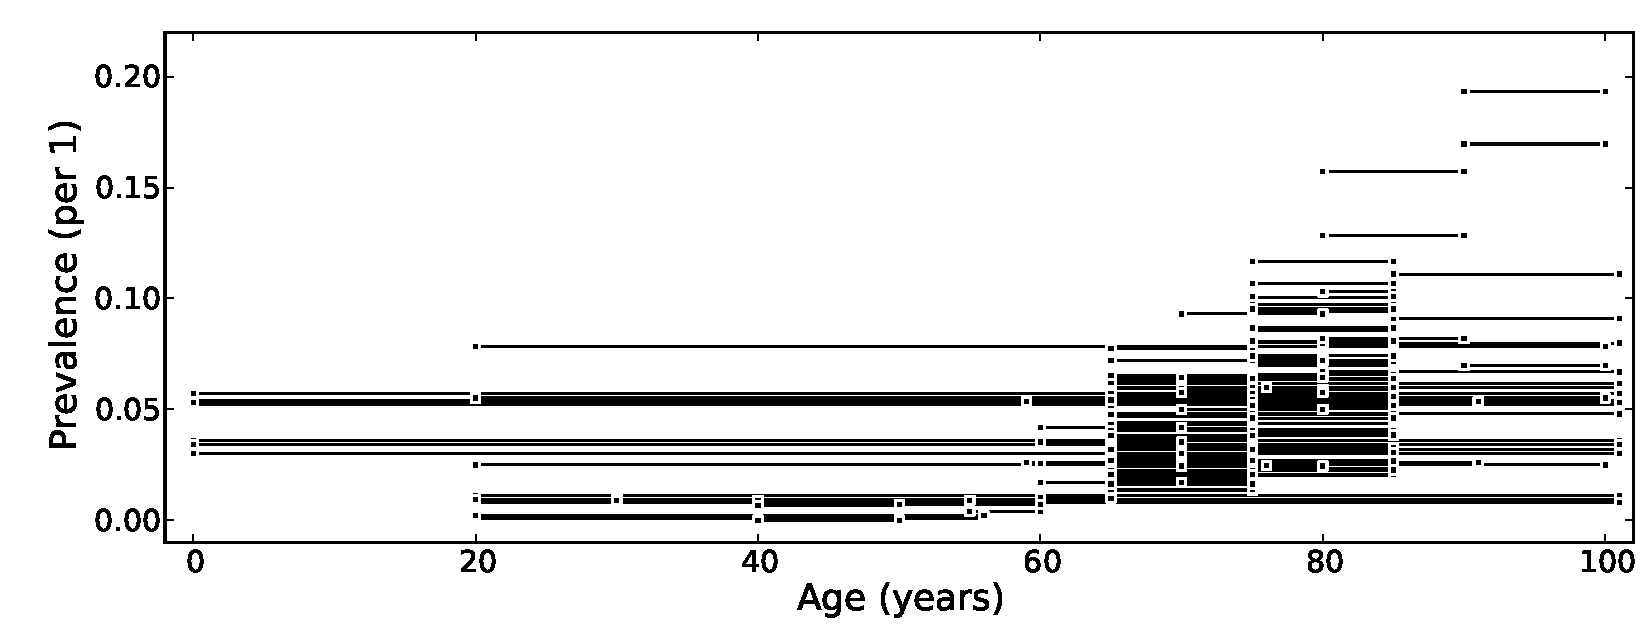
\includegraphics[width=\textwidth]{af_ages_intervals.pdf}
\caption{The systematic review of the descriptive epidemiology of
  atrial fibrilation included $155$ observations of disease prevalence for the United States.
 The prevalence level and age group of
  each observation is shown above as a horizontal bar, with the
  position of the bar along the $y$-axis representing the prevalence
  level and the endpoints along the $x$-axis representing the start and
  end of the age group.  The data shows heterogeneity by age that is
  typical for these systematic review results, which clearly increases with
 with age.  }
\label{theory-age_group_model-dismod_data_plot}
\end{center}
\end{figure}

Each of the horizontal lines in
Figure~\ref{theory-age_group_model-dismod_data_plot} can be
represented as a triple $({a_s}, {a_e}, r)$, where $a_s$ is the
starting age of the age group, $a_e$ is the ending age of the age
group, and $r$ is the rate observed for this age group.

A brief word about ${a_e}$ is in order here.  Often in the
epidemiological literature, the ending ages are described in a
unit-dependent fashion, for example age group 10-14.  This is intended
to mean from the first day of age 10 to the last day of age 14.
However, this notation can be a hindrance when dealing with age
resolution finer than one year, a situation that comes up when studying
neonatal conditions.  For this reason, I prefer the approach that
takes the end age of the interval to be the first age where an
individual is no longer part of the group.  In the case above, I would
say ${a_e} = 15$.


With a firm understanding of the sort of overlapping age group data
that arises in systematic review, I now turn to developing and
analyzing a series of models for the meta-analysis of the data.  There
are five that I will consider: the midpoint model, the disaggregation
model, the midpoint-with-covariate model, the age-standardizing model,
and the age-integrating model.  The age-standardizing model is the
balance of theoretical foundations, practical implementability, and
empirical success that is used in the second half of this
book.

\section{Midpoint model}

The simplest approach to modeling data with heterogeneous age
intervals, is to apply each rate measurement to the midpoint of the
age group it measured.  This is trivial operationally, but it is also
theoretically justified through a ``trapazoidal rule'' integration.

In practice, this approach is quite accurate for modeling a
disease rate that changes slowly as a function of age.  However, it
becomes inaccurate when modeling rates that change more
rapidly.  The typical setting in applications in the second half of
this book will include a few studies that focus on age patterns and
hence have narrow age groups, together with many other studies
that focus on other aspects of disease epidemiology.  Thus the
relevant setting to consider how these models are inaccurate is where
there are a few small age group studies and many large age group
studies.

Mathematically, the formulation is as follows: let $h(a)$ be a
process-model for the age-specific function (e.g a spline model
from Chapter~\ref{theory-age_pattern_model}, or the age-specific prevalence function derived from the solution to the system of differential equations from Chapter~\ref{sys-dynamics}), and let $\dens(r,n\given
\mu,\rho)$ be a data-model for the observed level (e.g the probability
density function for negative-binomial rate model from
Chapter~\ref{theory-rate_model}).
Then the likelihood of an observation of rate $r_i$ with effective
sample size $n_i$ for age group $({a_s}_i, {a_e}_i)$ is simply
$\dens\left(r_i, n_i \given h\left(\frac{{a_s}_i+{a_e}_i}{2}\right),
\rho\right)$. Equivalently, in ``blackboard notation,'' using
$\scD(\mu, \rho; n_i)$ to denote the rate model distribution, I can
write
\begin{align*}
r_i &\sim \scD\left(h(a_i), \rho; n_i\right),\\
a_i &= \frac{{a_s}_i+{a_e}_i}{2}.
\end{align*}
This formulation will be convenient for comparison with the other models of age groups to come.

To understand how accurately age group models like the midpoint model
can estimate, I used simulation.  The precise details are defered
until Section~\ref{agm-compare}, but, since this simulation is also used for the
figures that follow, I will describe it in brief here.  First, I
selected an age-specific hazard function as ground truth.  Then I
generated noisy measurements, from a mixture of regularly spaced
$10$-year age groups and uniformly random age groups.  For each
measurement, I chose a random population structure, and integrated the
true age-specific hazard to find the true rate for the age group.
Then I sampled from a negative binomial distribution with this true
rate as the mean, and a fixed overdispersion parameter to obtain noisy
data, which I used in the age group model.  Since ground truth is
known in this simulation, I can compare the model estimates to the
truth graphically as well as quantitatively.

Figure~\ref{midpoint} compares the estimate produced by the midpoint
model to ground truth through simulation using two different
age-specific hazard functions as ground truth.  When the age-specific
hazard varies little as a function of age, as shown in panel (a), the
estimated hazard function is quite accurate.  But when the age-specific hazard function
varies substantially, as shown in panel (b), the estimate is biased.


\begin{figure}[h]
\begin{center}
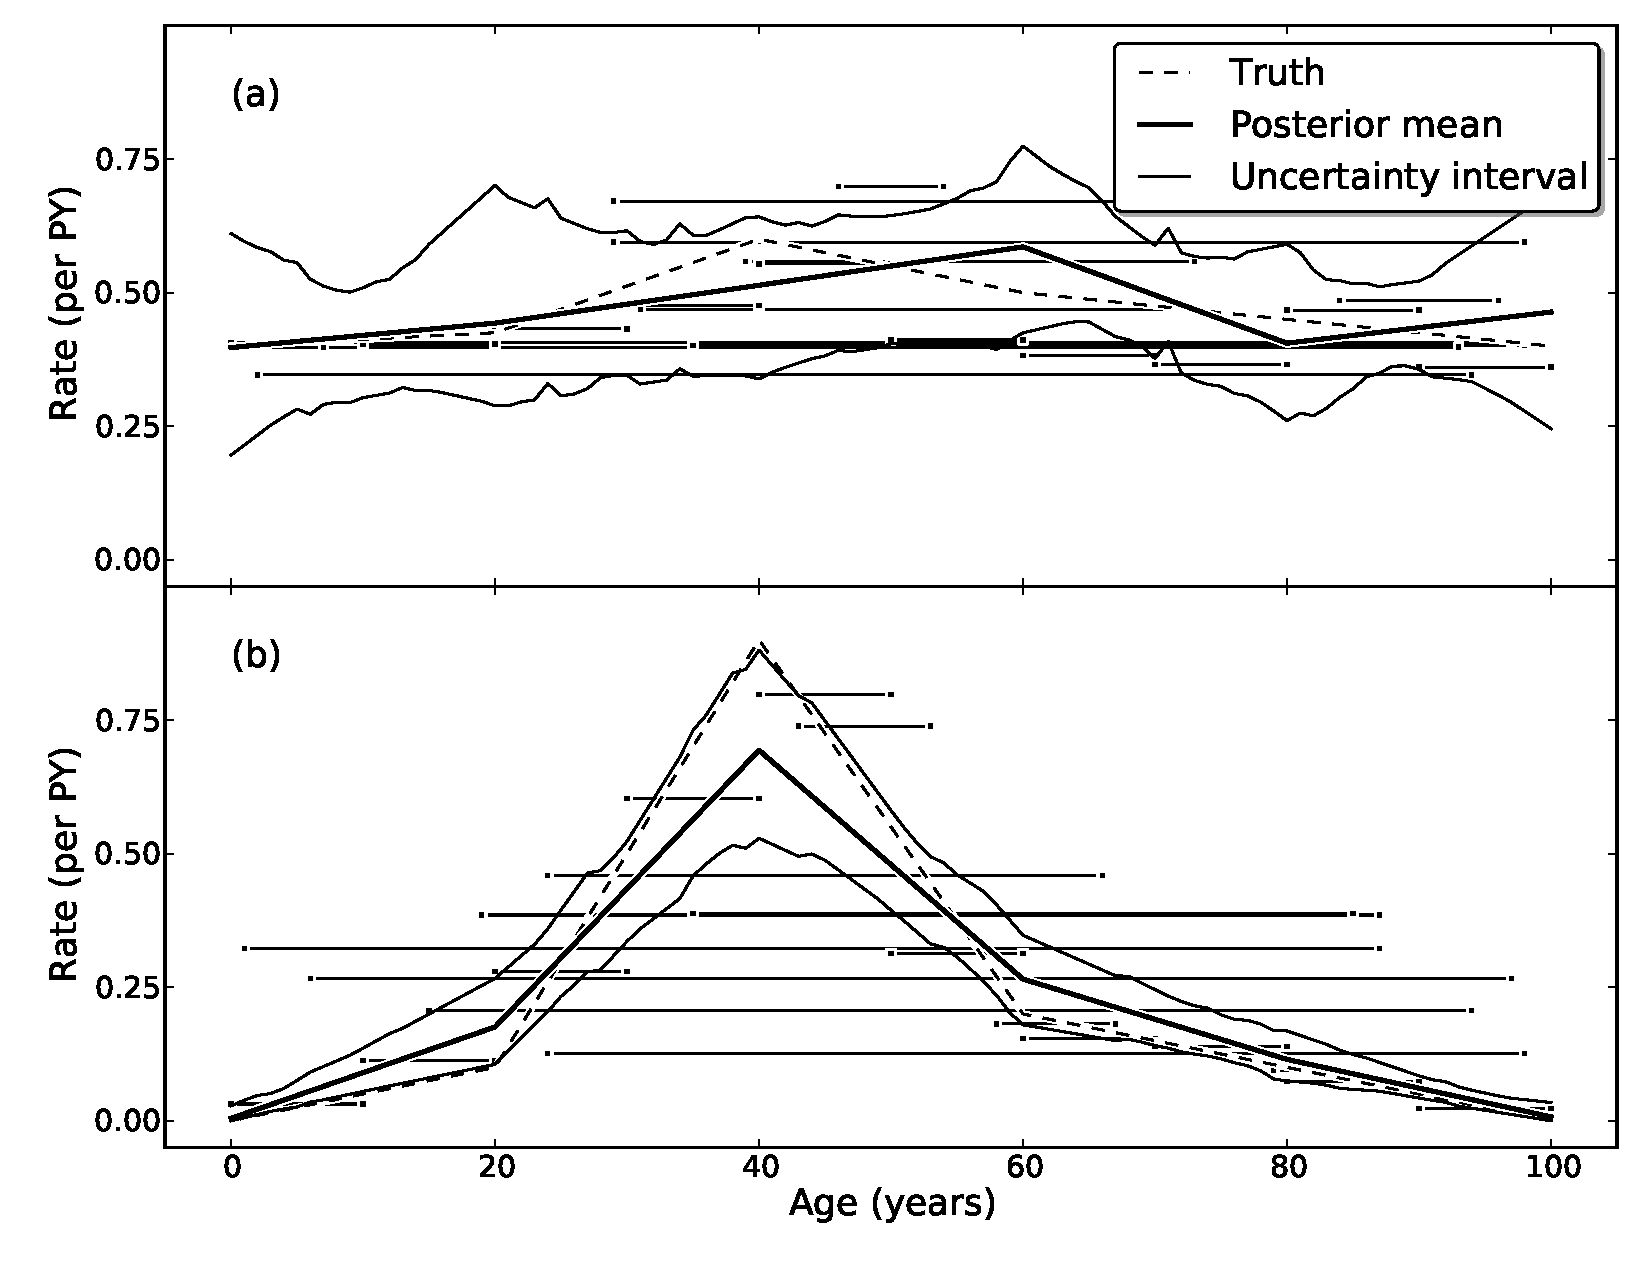
\includegraphics[width=\textwidth]{age_group_midpoint.pdf}
\caption{The midpoint model, a conceptually simple approach to
  dealing with data with heterogeneous age groups, simply
  attributes the observation to the midpoint of the age group.  Panel
  (a) shows the model applied to an age-specific hazard function that does not
  vary a great deal across ages for which the midpoint model is a
  better fit.  Panel (b) shows the model applied to an age-specific hazard function
  that varies more for which the midpoint model overcompresses the
  estimates.}
\label{midpoint}
\end{center}
\end{figure}


\section{Disaggregation model}
An alternative to the midpoint model which seems appealing but has
some downsides is what I call \emph{disaggregation}.  To understand
the disaggregation approach, imagine the simple re-analysis that I
could do if microdata were available (as described at the beginning of
this chapter).  If I had access to the individual measurements that
went into the calculation of the disease rate found in systematic
review, I could do a re-analysis with any age grouping I wished. I
could calculate rates for single-year age groups, and be sure that the
age pattern is not changing substantially during the grouping.

The microdata from rates found in systematic review are rarely
available, however. The disaggregation approach is a simple attempt to
impute what the rates for the desired age grouping would be \emph{if}
the microdata were available. This requires taking into account the
increased variation that would be found if a study of the same size
was reported for finer age groups.

Without any additional information, rate data reporting a level of $r$
for a population with effective sample size $n$ for age group $(a_s,a_e)$, i.e.,
\[
X = (r, n, a_s, a_e)
\]
can be disaggregated into $A = a_e-a_s$ rows of
data, $X_1, X_2, \ldots, X_A$, with 
\[ 
X_a = \left(r, \frac{n}{a_e-a_s}, a, a+1\right), \text{for } a=1,2,\ldots,A. 
\]

Disaggregation can be interpreted as a data preprocessing step, and
this disaggregated data can be fed to the midpoint model from the
previous section to produce a comprehensive estimate of the rate as a
function of age. However, this model has some unintended negative
features when large age intervals are disaggregated.  Because it
ignores the correlation in age of disease levels, it tends to
overcompress age patterns at young and old ages, as shown with simulated data in Figure~\ref{disagg}.

\begin{figure}[h]
\begin{center}
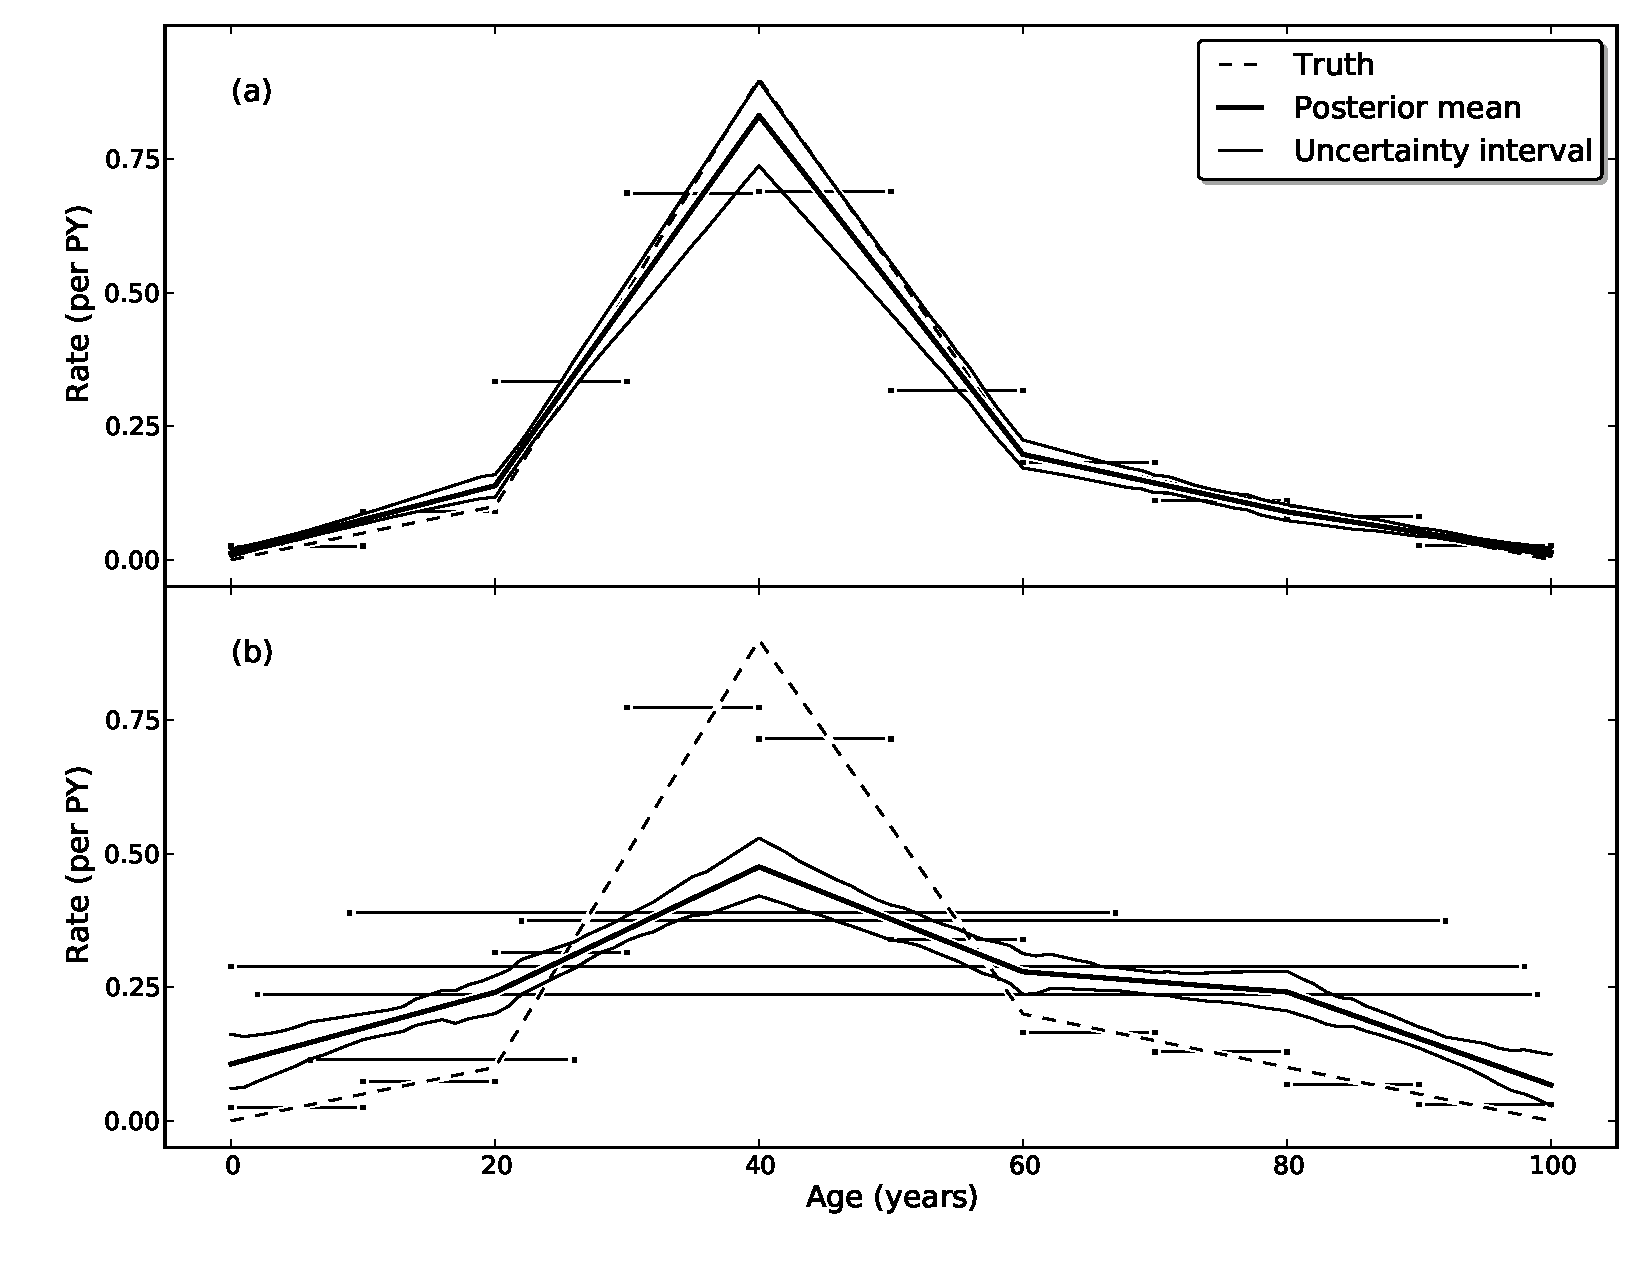
\includegraphics[width=\textwidth]{age_group_disagg.pdf}
\caption{This figure shows the effects of fitting a model with this
  disaggregation approach to two simulated data sets.  When the age groups are sufficiently
  fine-grained and homogeneous, disaggregation is a successful
  approach.  But with even slight heterogeneity, as in panel (b), the model
  estimates are overcompressed}
\label{disagg}
\end{center}
\end{figure}


\section{Midpoint model with group width covariate}
An alternative method, which I consider more ``statistical'' in its
approach, is to add the width of the age group as a covariate into the
midpoint model.  This model takes the form
\begin{align*}
r_i &\sim \scD\left(\mu_i, \rho; n_i\right),\\
\mu_i &= h\left(\frac{{a_s}_i+{a_e}_i}{2}\right) + \theta (a_e - a_s).
\end{align*}

This addresses the shortcomings of the disaggregation approach
\emph{indirectly}, and the indirect nature has positives and
negatives.  This method does not explicitly connect the large age
interval to the small age interval but instead allows the data to
inform the relationship.  On the other hand, it posits that the
data-driven relationship between the rates for studies with the same
midpoint but different age groups is a linear relationship. In
contrast, the mathematical model developed at the beginning of this
chapter is nonlinear in
a specific and mechanistically known way.
Figure~\ref{midpoint-covariate} shows the results of applying the midpoint-covariate model
model to simulated data.


\begin{figure}[h]
\begin{center}
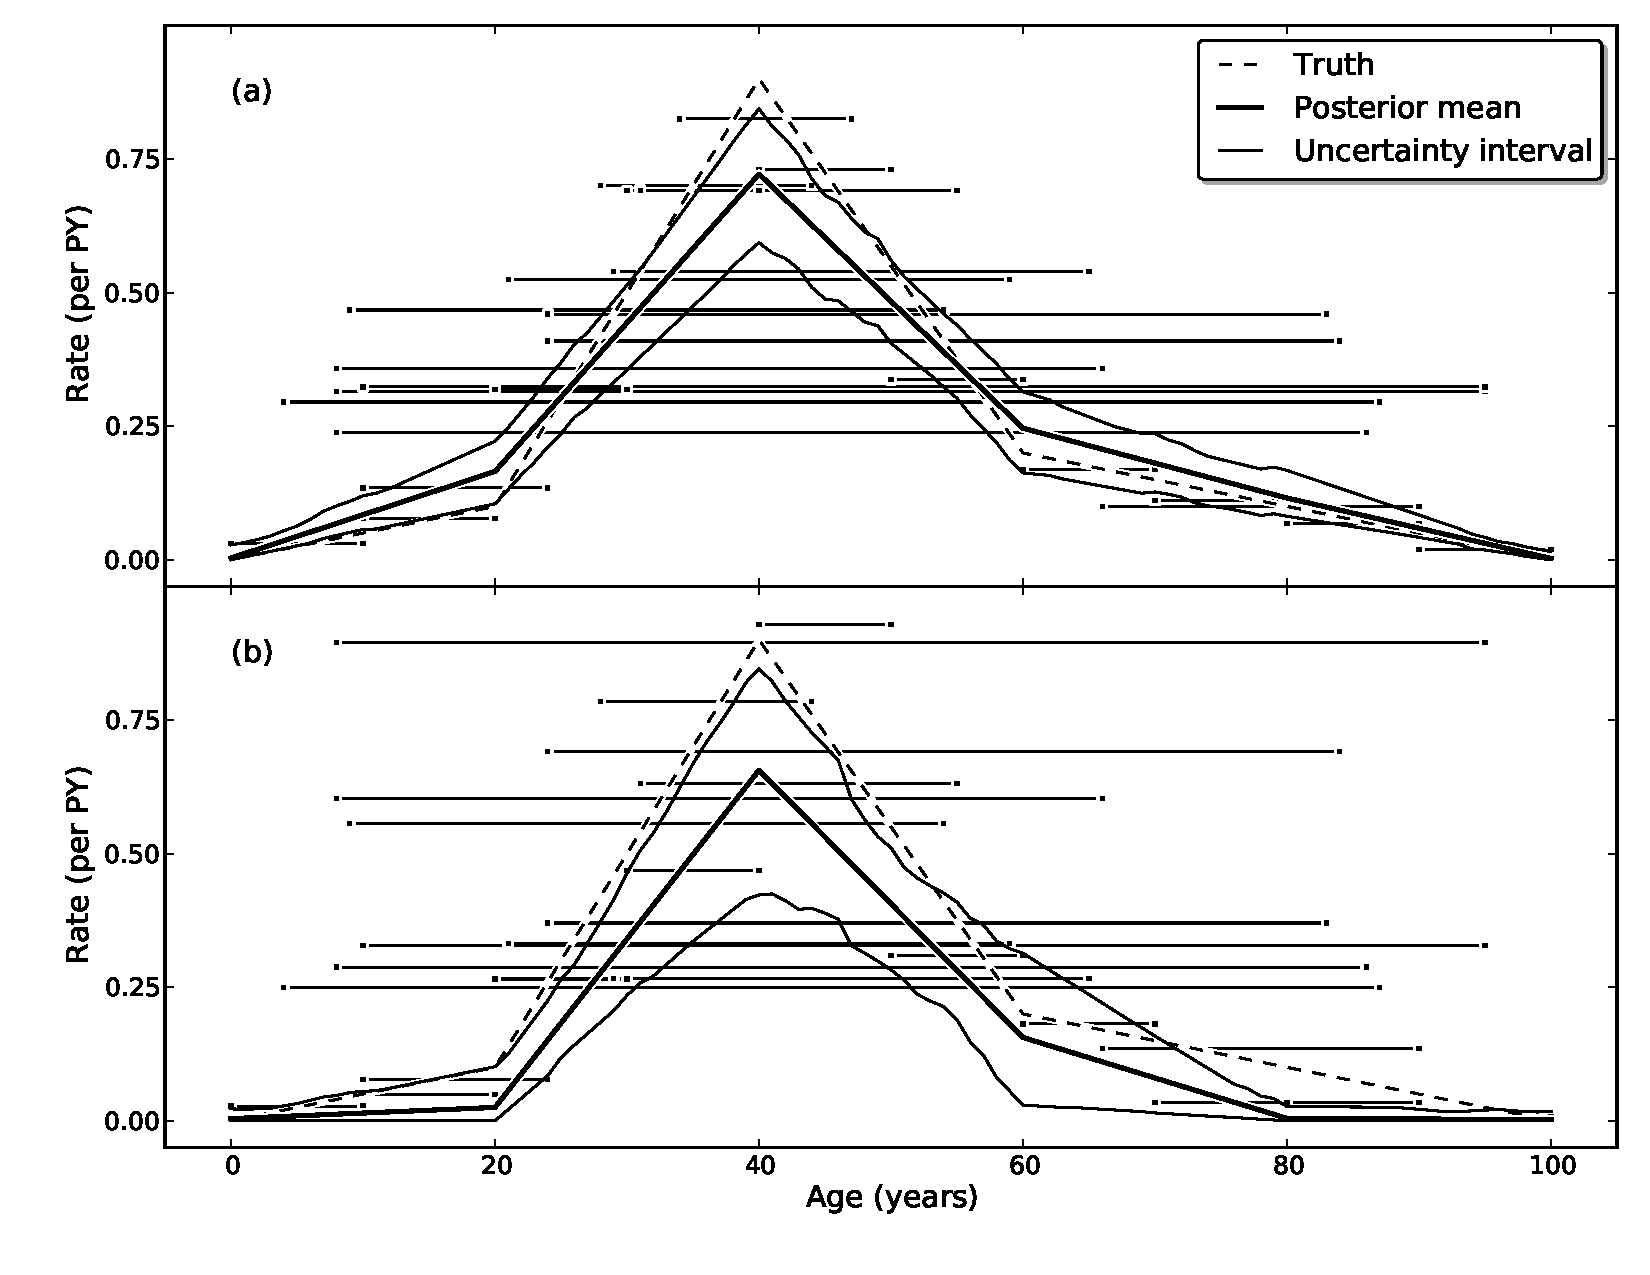
\includegraphics[width=\textwidth]{age_group_midpoint_covariate.pdf}
\caption{The midpoint-covariate model applied to two simulated
  datasets, where ground truth is known. Although this approach is
  appealing theoretically, the added flexibility of the covariate
  model does not add much value in the simulation study. }
\label{midpoint-covariate}
\end{center}
\end{figure}

\section{Age-standardizing and age-averaging models}
An even more complicated approach, both conceptually and
computationally, is to average across the age interval explicitly in
the statistical model:
\begin{align*}
r_i &\sim \scD\left(\mu_i, \rho; n_i\right),\\
\mu_i &= \int_{a={a_s}_i}^{{a_e}_i} h(a)\d w_i(a),
\end{align*}
where the integration $\d w_i$ is weighted according to population
structure.

This has the theoretical appeal of matching the generative model above
but the drawback of being slower to compute and less stable
numerically.  It also has a major piece left unspecified, the
selection of the age weights for the integration.  There are two
sensible approaches to this, which I call the \emph{age-standardizing
  model} and the \emph{age-averaging model}.  The age-standardizing
model uses a common age pattern $\d w_i(a) = \d w(a)$ for all studies, while
the age-averaging model uses the best estimate available of the age
pattern of the study population in each observation.  The
age-standardizing model is faster, due to a computational optimization
only possible when the $\d w_i$ are the same for all $i$, but the
age-averaging model is appealing on theoretical grounds, because it
can make use the most information.  However, it is not certain that
using this information will make the end results any more accurate,
because the age pattern of the study population is rarely known with
much certainty, and often it is necessary to assume that it matches
the national age pattern for the country-years where the study was
conducted.  In the case of remission and mortality studies it is even
more complicated to estimate the study population age pattern, since
it is \emph{not} the same as the national population age pattern, but
modulated by the age pattern of disease prevalence.
Figure~\ref{age-group-standardize} shows the results of this model on
simulated data.

\begin{figure}[h]
\begin{center}
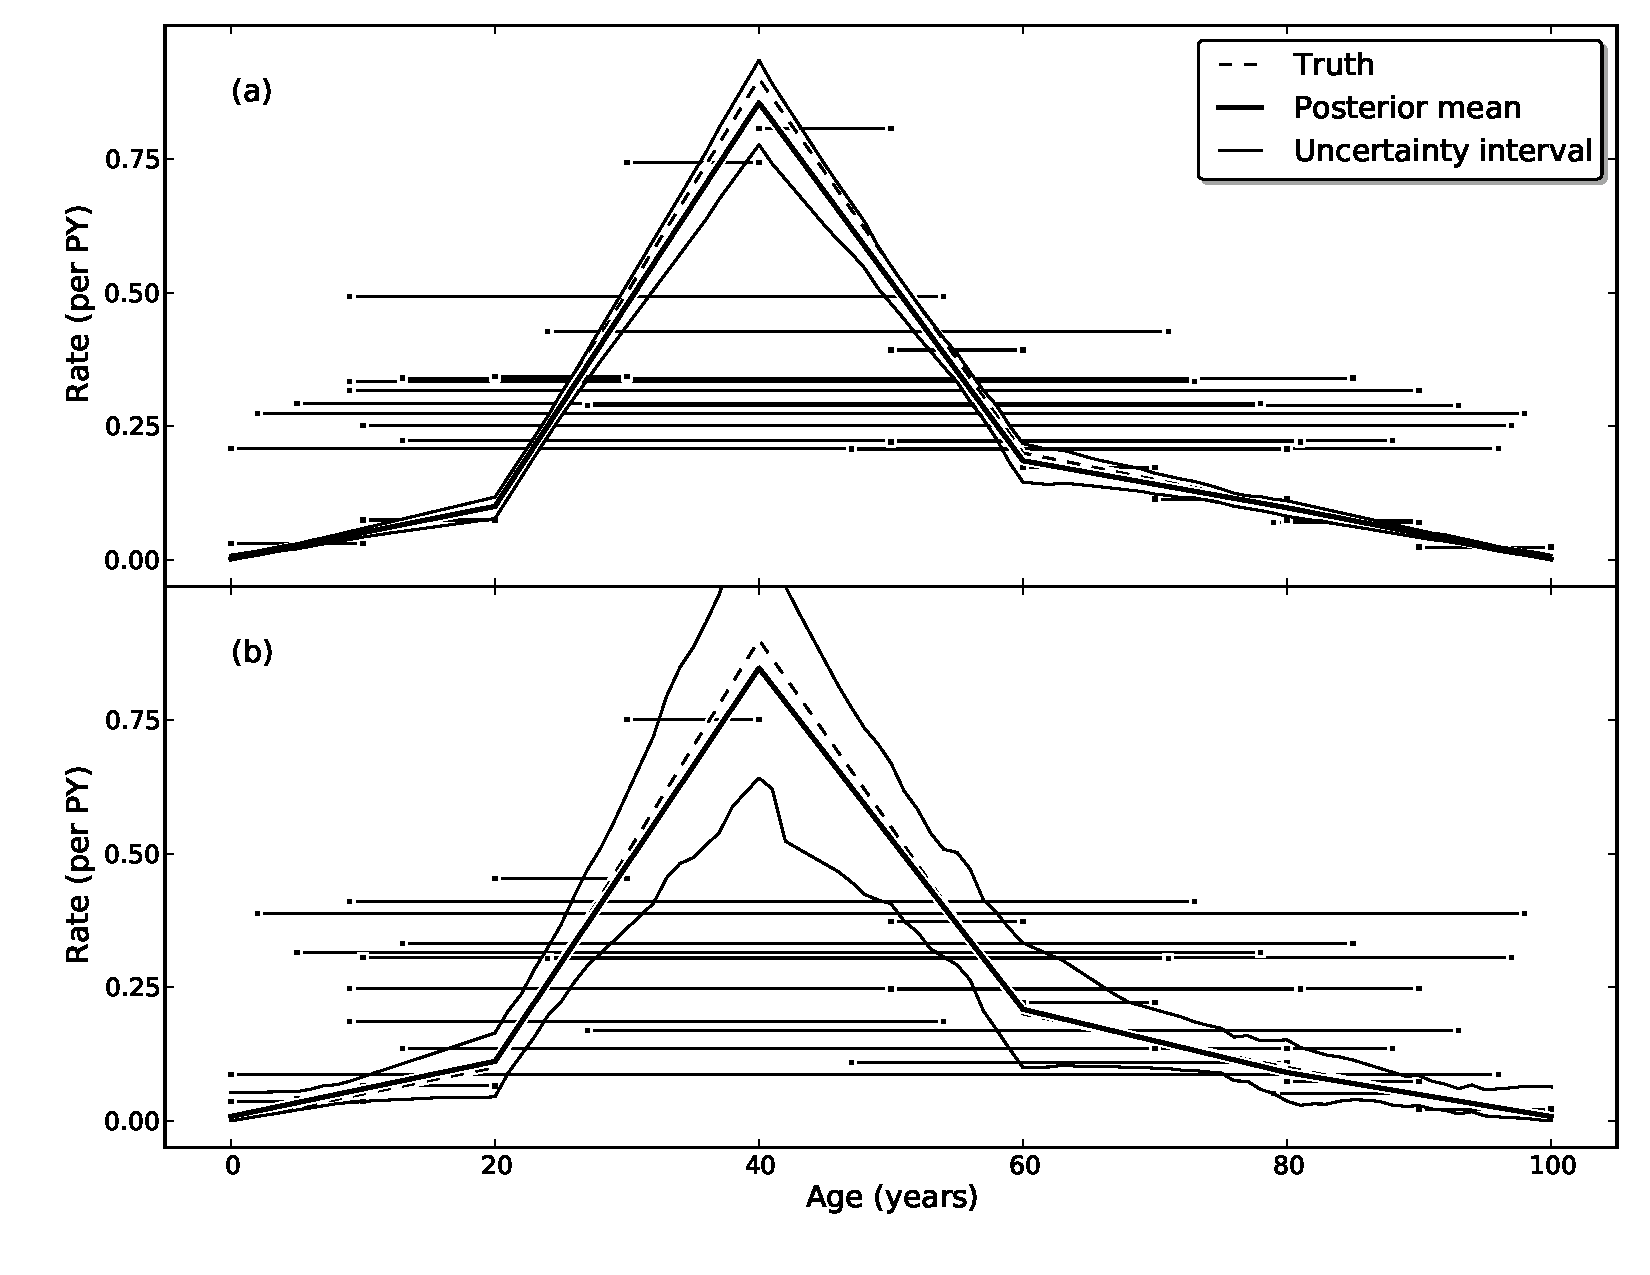
\includegraphics[width=\textwidth]{age_group_standardize.pdf}
\caption{The age-standardizing model applied to simulated data with a
  known age-specific rate function as ground truth.  The results in
  panel (a) show that the model 
  recovers the true age pattern quite precisely. Panel (b) shows that the
  results are still accurate when the data generation procedure is
  even more noisy.}
\label{age-group-standardize}
\end{center}
\end{figure}


\section{Model comparison}
\label{agm-compare}

\begin{figure}[h]
\begin{center}
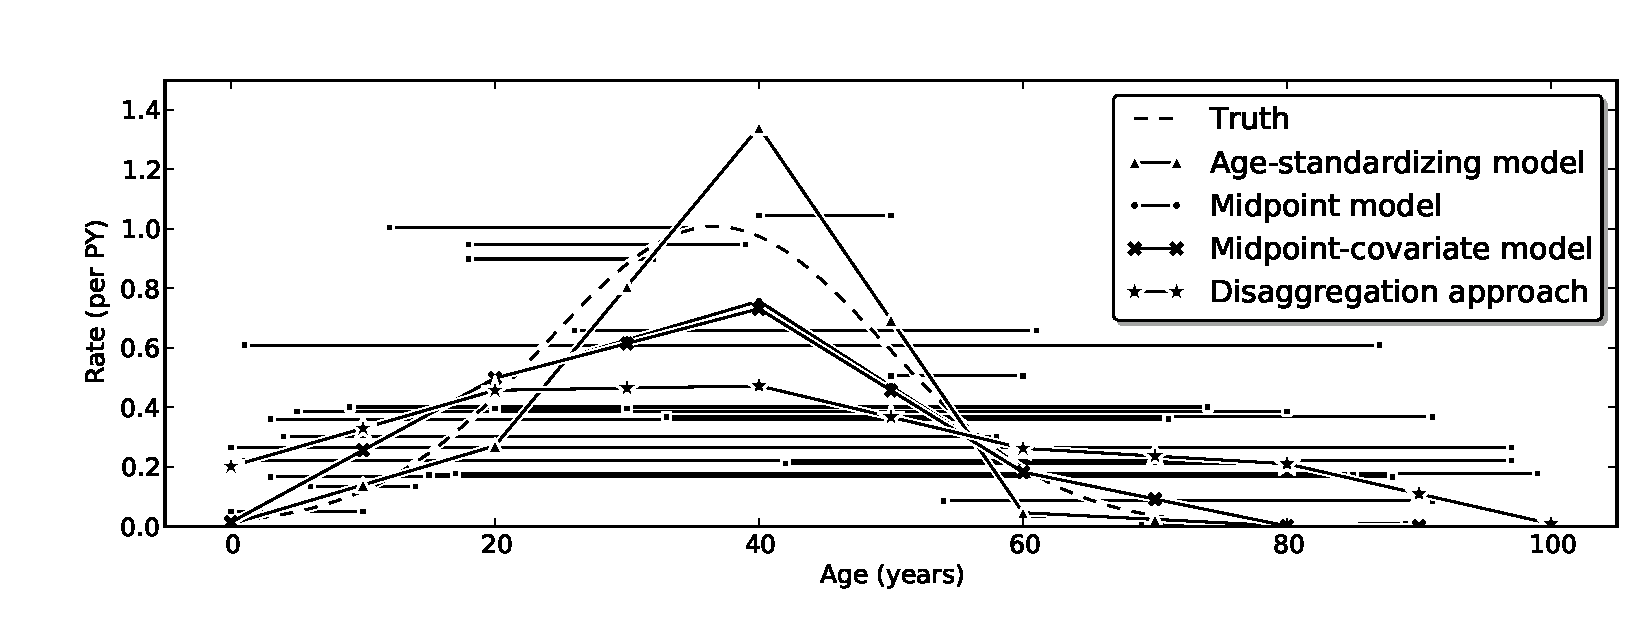
\includegraphics[width=\textwidth]{age_group_models.pdf}
\caption{A comparison of $4$ models for heterogeneous age groups, showing that the age-standardizing model comes closest to recovering the truth.  This corresponds to the results of the simulation study presented below in Table~\ref{age_group_comparison}.}
\label{age-group-model-comparison}
\end{center}
\end{figure}


This section provides a comparison of the approaches to age group
modeling.

An appropriate comparison of these approaches is somewhat difficult to
develop.  One approach is through simulation study, where a dataset is
simulated from known ground truth.  This allows the estimates to be
compared to ``true'' values, but this risks
inappropriate model selection due to inaccurately choosing the
distribution of the simulated data.  Another approach is
cross-validation, where data from systematic review is split into
mutually exculsive
\emph{training} and \emph{test} sets, and the model is fit to the
training set and used to predict the values in the test set.  Naively
holding out $25\%$ of the data doesn't address the exact topic of
interest, however, since it determines which model predicts rates of
all age groups, and I am really only interested in predicting the age
groups with small widths accurately.  It would be preferable to hold
out only data with small-width age groups from large representative
subpopulations.  Unfortunately there is rarely enough data to do this,
especially in all the settings that come up in disease modeling.

I have taken a pragmatic approach, evaluating with a natural
simulation described below.  Future work, based on more sophisticated
simulation scenarios or based on carefully designed hold-out
cross-validation, is necessary to further understand the trade-offs
between these alternative methods.

The data simulation procedure I used is the following:
\begin{itemize}
\item Choose age intervals for $30$ rows of data; for $i=1,\ldots,10$,
  $({a_s}_i,{a_e}_i) = (10(i-1), 10i)$, and for the remaining $20$
  intervals, choose the age interval width uniformly at random from $[1,100]$
  and choose the midpoint of the age interval uniformly at random from ages
  which admit this age range.

\item Choose the effective sample size $n_i$ for each row, uniformly at random from $[10^2, 10^4]$.

\item Choose an age-specific population structure for each row of data,
  with the form $w_i(a) = e^{\beta_i a}$, where $\beta_i$ is drawn
  from a normal distribution with mean $0$ and standard deviation
  $\frac{1}{10}$.

\item Calculate the true rate value for each age interval,
  $r^\text{true}_i = \sum_{a={a_s}_i}^{{a_e}_i} \mu_\text{true}(a)
  w_i(a)$, where $\mu_\text{true}(a) =
  \exp\left(\frac{3(a-35)^2}{1000} + \frac{a-35}{100}\right).$

\item Choose an observed rate value, based on a negative binomial distribution:
$r_in_i \sim \NegativeBinomial(r^\text{true}_i, \delta_\text{true})$, where $\delta_\text{true} = 5$.
\end{itemize}

Table~\ref{age_group_comparison} shows the median results of fitting this simulated data with a variety of models.

\begin{table}

\begin{center}
\begin{tabular}{|c|c|c|c|c|}
\hline
model&bias&mae&pc&time\\
\hline
midpoint&0.02&0.08&0.8&29.0\\
disaggregation&0.03&0.19&0.08&52.6\\
midpoint-covariate&0.03&0.09&0.89&45.8\\
age-standardizing&0.01&0.04&0.95&30.3\\
age-integrating&-0.0&0.03&0.78&38.1\\
\hline
\end{tabular}
\end{center}

\caption{Median results for $100$ replicates of the simulation study
  comparing age-specific rate estimates from $5$ models of age-grouped
  data, showing bias (mean of true minus predicted), median absolute
  error (mae, median of absolute difference between truth and
  predicted), probability coverage (pc, fraction of truth falling
  within 95\% uncertainty interval of prediction), and computation time. The
  age-standardizing and age-integrating models are superior in all
  metrics of fit quality.  The age-standardizing model has computation time only slightly more
  than the fastest approach, while the age-integrating model is 26\% slower.}
\label{age_group_comparison}
\end{table}

\chapter{Covariate modeling}
\label{theory-covariate_modeling}
As I have mentioned frequently in previous sections, the
epidemiological data on disease morbidity collected in systematic
review is often very sparse and very noisy.

Covariate modeling is a method to explain the noise in noisy
data in terms of demographic, epidemiological, and study-specific
variables.  This is often challenging because there is no particular
explanatory variable available, and also because the data are very
sparse.  Nonetheless, this approach has a long history of relevant
application in global health \cite{Girosi_Demographic_2008,Wakefield_Bayesian_1996}.

In the integrative systems model of disease in populations, covariate
modeling has two distinct goals.  One is covariates are a way to
explain the bias and variation of the noisy measurements of
epidemiological rates.  For example, covariates can be used as a mechanism
for data-driven ``cross-walks'' between alternative diagnostic methods
that have different sensitivities, and can also be used to 
down-weight data that comes from a noisier source such as
from nonrepresentative subpopulations that are not systematically
biased above or below the mean.

The other goal in covariate modeling is to use covariates as a
mechanism to increase the accuracy of out-of-sample predictions.  This
is accomplished by modeling the relationships between the disease
parameters of interest and the explanatory covariates. The modeled
relationships are then used to extrapolate predictions for the disease
parameters to geographic regions where covariate data is available,
but no direct measurements are made.

In covariate modeling, there is often a distinction made between
``fixed effects'' and ``random effects.''  Bayesian approaches, such
as hierarchical modeling, blur this distinction (to the point that
hierarchical modeling is somtimes called ``mixed effect'' modeling
\cite{Gelman_Multilevel_2005}.  To make the nomenclature more
complicated, different methodological traditions of covariate modeling
have opposite concepts of what is fixed and what is random in effects.

For integrative systems models of disease, I make the following
distinction between fixed effects and random effects: while fixed
effects have covariates that may vary by study or by country-year,
random effects have geographic unit indicators as covariates only.
Sometimes I constrain random effects to sum to zero at each level of
the geographic hierarchy, which is an extension of the traditional
meaning of random effects in linear regression, where the population
mean of a random effect is zero.  In other models, it is sufficient to
use a prior with mean zero for the random effects.  In either case,
my random effects always have a hyper-parameter for the dispersion,
which allows the model to infer how dispersed the random effects are
between geographic regions, and hence quantify the uncertainty in the
geographic regions for which no data is available.

These concepts will all be elaborated on in turn in the following
sections of this chapter.

\section{Fixed effects to explain bias}

A prototypical example comes from myocardial infarction (MI)
incidence, where there are a variety of diagnostic tests available and
different studies of prevalence use different diagnostic criteria
for case ascertainment.  The newer class of tests, which are based on
measuring levels of the blood protein troponin, are more sensitive
than earlier methods, and this leads to variation in data with a clear
explanation.  Figure~\ref{cov-sim} shows simulated data with a
covariate that has an effect like a troponin-based test might, raising
the number of observed cases by 30\%. By including an indicator
variable as a covariate in each row of data, $x_i = 1$ if row $i$
comes from a study that used a troponin test, and $x_i = 0$ otherwise,
I can fit a model which includes a parameter to cross-walk between
studies using these two different case ascertainment criteria.

\begin{figure}[h]
\begin{center}
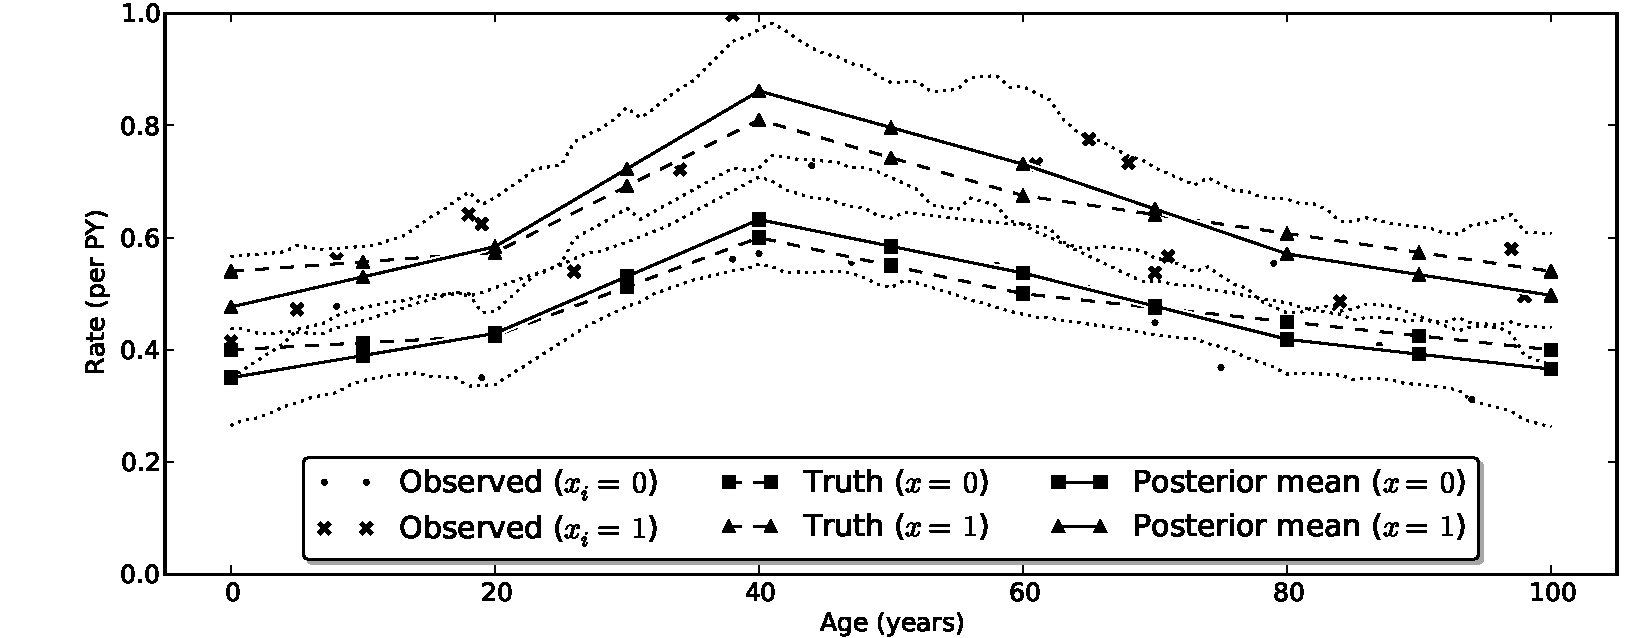
\includegraphics[width=\textwidth]{cov_fe.pdf}
\caption{Simulated dataset where different measurement techniques
  yield systematically different values. The data with $x_i=1$ are on
  average 30\% higher than data with $x_i=0$, and the covariate model
  recovers this difference accurately, with sufficient data.}
\label{cov-sim}
\end{center}
\end{figure}

This same approach can be applied to data on psychological disorders for gathered with alternative
recall periods, an application that arises frequently in the
meta-analysis of psychological disorders.  For example, in measuring
the population prevalence of bipolar disorder, many studies ask about
the existance of symptoms in the past month, while many others ask
about the past year.  Figure~\ref{bipolar-data-cv} shows the data
collected in systematic review for bipolar disorder, where past year
prevalence is higher than past month prevalence, because of the
episodic nature of the condition.

\begin{figure}[h]
\begin{center}
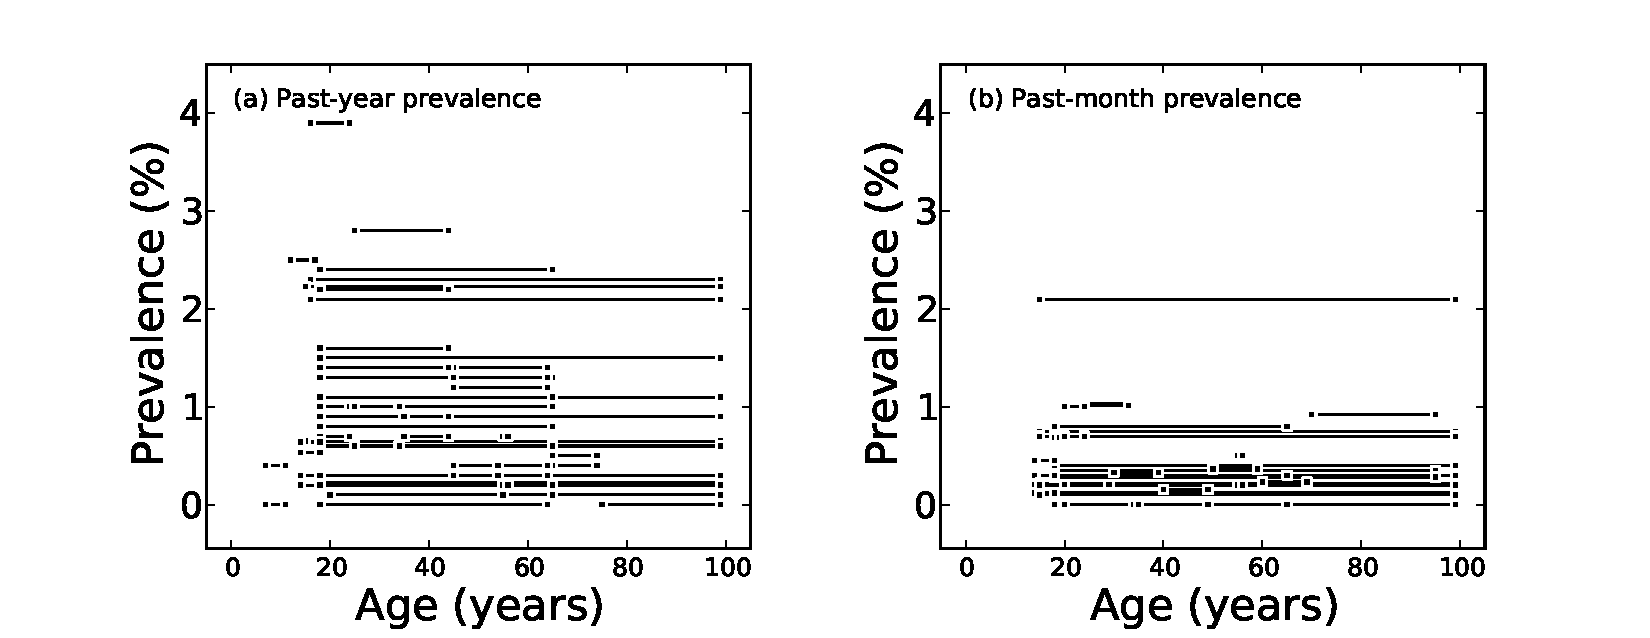
\includegraphics[width=\textwidth]{bipolar-data-by-cv.pdf}
\caption{Data on bipolar disorder collected in systematic review.
  Some studies measured past year prevalence, while others measured
  past month prevalence.  Because of the episodic nature of the
  condition, past month prevalence is $30$ to $40\%$ lower than past
  year prevalence.}
\label{bipolar-data-cv}
\end{center}
\end{figure}


In general, let the data collected in systematic review be denoted by
tuples $\left(a_i, n_i, r_i, X_i\right)$, where $a_i$ is the age
group, $n_i$ is the effective sample size, $r_i$ is the observed rate
value, and $X_i$ is a vector of covariate values. Then, using
$\scD(\pi, \rho; n_i)$ to denote the rate model, the fixed-effect
covariate model is then the following:
\begin{align*}
r_i &\sim \scD\left(\mu_i, \delta; n_i\right),\\
\mu_i &= \boldmu(a_i)e^{\beta X_i}
\end{align*}

The parameter $\beta$ represents the effect coefficients for
the fixed effects, and because the data are often sparse and noisy, it
can help the stability of the computational algorithms to put a weakly
informative prior on $\beta$, such as
\[
\beta_j \sim \Normal\left(0, 1^2\right) \text{ for } j = 1, \ldots, J.
\]
Of course, if experts have beliefs about the sign or magnitude of the
effect coefficient, this can be included as a more informative prior.

Two subtle choices are worth additional investigation in fixed effect
modeling: reference values and normalization.  Both of these choices
are known to influence the performance of computational
algorithms \cite{gelman_bayesian_2003}. For example, nonnormalized covariates can produce
nonconvergence in hill-climbing algorithms that work fine with
normalized covariates.  But because of the Bayesian priors and
especially because of the consistency from the compartmental model,
the choices are particularly important in this setting.

The term \emph{reference value} is borrowed from fixed effects
modeling of categorical variables, where so-called dummy variables
(zero/one indicators) are introduced for all but one category. When
all the dummy covariates are set to zero, the model produces
predictions for the reference category. In the formulation above, the
analogous notion occurs when $X_i = (0, 0, \ldots, 0)$.  Then the
expression for $\mu_i$ simplifies to
\[
\mu_i = \boldmu(a_i) e^{\beta \0} = \boldmu(a_i).
\]
It is this $\boldmu$ that is used as the age-specific rate function in
the compartmental model (as developed in
Chapter~\ref{theory-system_dynamics}), so the consistency between
incidence, prevalence, remission, and mortality is enforced at the
reference values.

Because the reference values are consistent, they must be chosen with
care.  For example, in the case of MI above, where some studies used
troponin based diagnostics and some did not, the reference value
should be \emph{with} troponin tests, because this is considered to be
more accurate.

A concrete example using the bipolar disorder data can make this
clearer.  Chapter~\ref{bipolar} develops the consistent model for
bipolar disorder in detail, which is used here in two variations.
First, when the past year prevalence is used as the reference
value, and second when the past month prevalence is used as the
reference.  This changes the predicted prevalence, of course, but it
also changes the predicted incidence (for which little data is
available).  Figure~\ref{bipolar-ref-alts} shows how the alternative
reference values change the incidence estimate in this case.


\begin{figure}[h]
\begin{center}
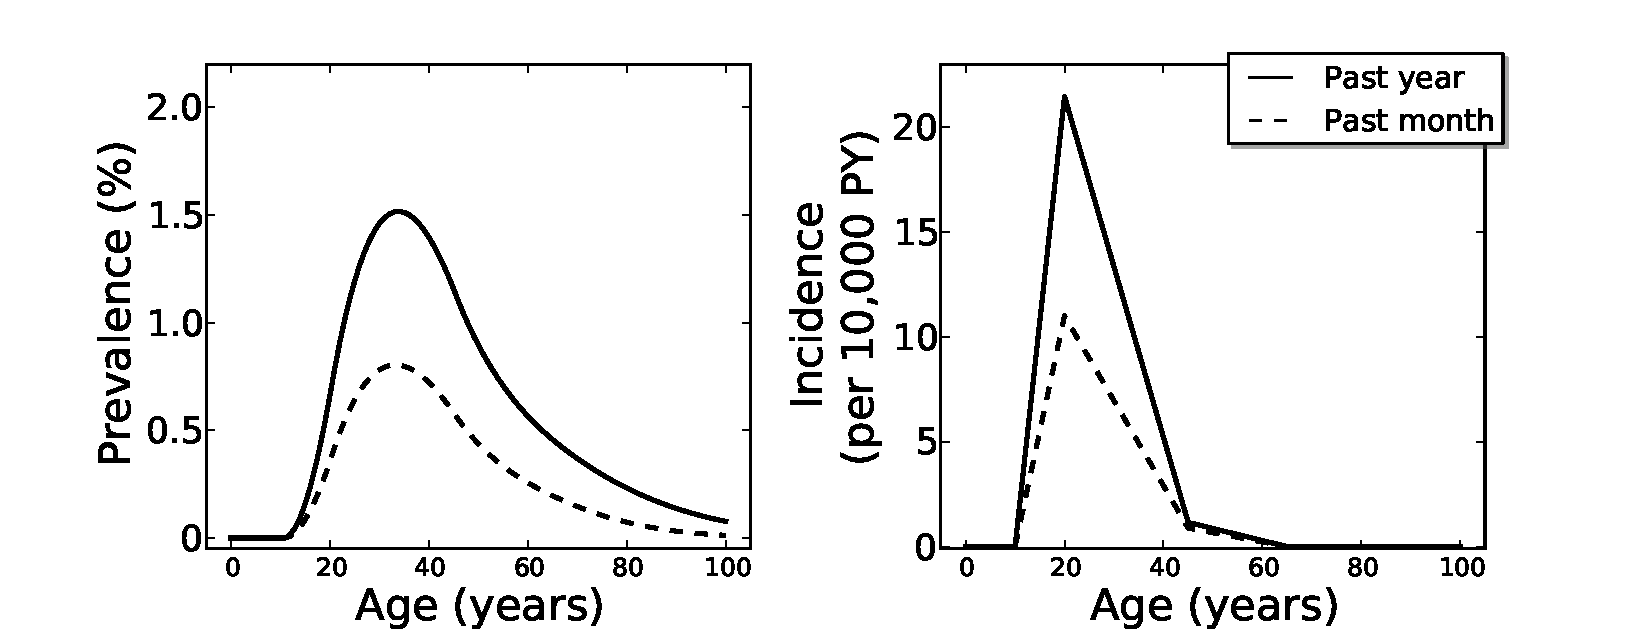
\includegraphics[width=\textwidth]{bipolar-ref-alts.pdf}
\caption{Reference value for the past year/past month prevalence
  covariate has a substantial effect on incidence estimates.  Because
  consistency is enforced at the reference value level, choosing reference
  values is an important modeling decision.}
\label{bipolar-ref-alts}
\end{center}
\end{figure}


Normalization is also important, although it does not affect
consistency.  It is important for stability of numerical algorithms,
and also because the prior on the effect coefficient must be matched
to the scale of the covariate.  Normalizing continuous covariates to
have variance one, for example, means that the prior of
$\beta\sim\Normal(0,1^2)$ is weakly informative.  If a continuous
covariate had variance $0.0001$, the same prior on $\beta$ would be
very informative.

\section{Fixed effects to predict out of sample}

In addition to study-level covariates, like the cross-walks in the
previous section, covariate modeling can be as ``country-level
covariates'' to improve prediction out-of-sample.  Mathematically, the
setting is identical, where a column of the data matrix $X_{ij}$ holds
the value of the covariate, and an effect coefficient parameter
$\beta_j$ modifies the prediction, multiplying it by
$e^{\beta_j X_{ij}}$.  Conceptually, this deserves a seperate treatment,
  however, because the use and the results are quite different.

A case where the benefit of using fixed effects to predict out of
sample is clear is when modeling an often fatal condition, like cancer
of the pancreas.  Incidence of pancreatic cancer is available from
cancer registries for some regions, but population-level mortality
caused by this condition has been modeled in detail for all
countries.  By using the log of the age-standardized mortality rate as a
covariate in the incidence model, it is possible to borrow strength
from the mortality estimates to inform the incidence estimates.

This approach can also be helpful for covariates that are not as
direct, for example using gross domestic product as an explanatory
covariate for estimating the prevalence of eating disorders, using
estimates of age-standardized Hepatitis C Virus prevalence as an
explanatory covariate for estimating prevalence of cirrhosis, or using
an indicator for violent conflict as an explanatory covariate for
estimating the prevalence of depression or anxiety.



\section{Fixed effects to explain variance}
Fixed effect modeling in the previous sections has focused on
improving predictions of the mean of observed data.  It is also
possible to use fixed effect covariate modeling to explain the
different levels of variation in different sources of data, which is
the topic of this section.

To introduce this idea by way of example, consider the results of the
systematic review for Hepatitis C Virus seroprevalence.  This
literature search excluded studies in subpopulations known to have
systematic bias, such as studies of prevalence in intravenous drug
users, or paid blood donors.  But it did collect measurements from
studies in subpopulations that were \emph{not} know to be
systematically biased, for example studies that used voluntary blood
donors as the sample frame.  This is clearly not the whole population,
but as it is not known to be a biased sample, I would like to include
it if possible.  This is where using a fixed effect to explain
variation is appropriate. In the systematic review, observations corresponding
the voluntary blood donors, as well as other studies of nonrepresentative
subpopulations, such as mothers visiting antenatal clinics, were
associated with a
bias indicator $z_i = 1$.  Observations from studies of the general
population received bias indicator $z_i = 0$.  Then I can 
introduce fixed effect coeficient analogous to the previous sections,
but modifying the over-dispersion term of the rate model, instead of
the mean.

This has the following
formulation:
\begin{align*}
r_i &\sim \scD\left(\mu_i, \delta_i; n_i\right),\\
\mu_i &= \boldmu(a_i)e^{\beta X_i},\\
\delta_i &= e^{\eta + \zeta Z_i}.
\end{align*}

\section{Random effects for spatial variation}
Another important use of covariates is in handling nonsampling
variation that \emph{cannot} be explained. As I have mentioned
repeatedly, the descriptive epidemiological data available is often
very noisy.  It is usually only a small part of this ``noise'' that
can be explained with covariates like those from the preceding
section. And while the additional variation has no simple explanation
in terms of differing diagnostic criteria or the like, there is
structure in the variation. Countries in the North Africa/Middle East
region have rates more similar to each other than to countries in the
North America, High Income region.  And the North America, High Income
region as a whole is more similar to the Europe, Western region than
to the Asia, South region.  Capturing this spatial similarity when it
exists is the goal in my random effects modeling.

I will develop this approach to random effects modeling by beginning
with something very similar to the fixed-effects model.  The random
effects come in part through the use of additional priors, either
modeling the dispersion of the effects as a parameter itself, to be
fit from the data, or going further to model the join distribution of
spatially neighboring effects to have sums equal to zero.  For
notation, let $U_i$ be a vector of random effect covariates.  This
$U_i$ is a \emph{design matrix} analogous to the fixed-effect
covariate vector $X_i$ above, but with zero/one values corresponding
to the place in the spatial hierarchy to which observation $i$ refers.

In the GBD 2010 study, the spatial hierarchy is countries nested in regions
nested in super-regions, but in national or subnational analyses, the
hierarchy will be different. This can be generically formulated using
graph theory, where a directed tree (also known as an
\emph{out-arborescence}) encodes the hierarchical relationship
structure with a root node connected by out-arcs to children on the
first level of the hierarchy, which are each in turn connected by
out-arcs to children on the next level of the hierarchy, and so on.  A
node is called the \emph{parent} of any node it points to in this
tree, and two nodes are called \emph{siblings} if they share the same
parent.


Analogously to the fixed effect model above, the random effects apply
a multiplicative shift to the age-specific rate function:
\begin{align*}
r_i &\sim \scD\left(\mu_i, \delta_i; n_i\right),\\
\mu_i &= \boldmu(a_i)e^{\alpha U_i}.
\end{align*}
The first difference between the fixed effects and random effects is
in the priors on the effect coefficients.  Instead of a weakly
informative prior as above, the prior on $\alpha$ is itself part of
the model, parameterized as:
\[
\alpha_j \sim \Normal\left(0, \sigma_{\ell(j)}^2\right),
\]
where $\ell(j)$ is the level in the hierarchy of node $j$, and
$\sigma_\ell$ is also a model parameter. To fit this model with
Bayesian methods, we also need a prior on $\sigma_\ell$ (a
hyper-prior), and because of the sparse and noisy nature of the
available data, this often has to be somewhat informative.  The
truncated normal distribution
\[
\sigma_\ell \sim \Normal_{[.05,5]}\left(.05, .03^2\right),
\]
is often an appropriate choice. It says that between-area variation of
less than 5\% is impossible and more than 15\% is rare.

A second difference between the fixed effects and random effects which
I have sometimes found convenient is
the following: for every node in the spatial hierarchy, I can
constrain the random
effects for all children of that node to sum to zero.  This ``zero-sum
random effect'' has the implication that if there
are no data for some node, then its random effect must be zero.  It
captures the modeling philosophy that random effects represent
unexplained, but true, variation of nodes in the area hierarchy from
the central tendency of their siblings.  Using $H$ to denote the
hierarchy, this constraint can be formalized mathematically as:
\begin{align*}
\sum_{c\in N^+(p)} \alpha_c &= 0, \text{ for all } p \in N;\\
\alpha_c &=0, \text{ for all $c$ such that } \sum_{i} U_i(c) = 0.
\end{align*}

The zero-sum constraint has important implications in consistent
models, because as described above (and shown in
Figure~\ref{bipolar-ref-alts}), consistency is enforced at the
reference level, which for random effects is $U_i = \0$.


\section{Covariates and consistency}
One of the most challenging theoretical issues in covariate modeling
for integrative systems modeling is the interplay between the
predictive covariates and the intercompartmental consistency.  A
simple example of the problem arises in a model of congenital
abnormalities, where there is birth prevalence, but no incidence or
remission, and data on prevalence and cause-specific population
mortality. If covariates are used to shift predictions for the level
of $pf$ as well as the level of $p$ and the level of $f$, then
consistency would require that $\beta^{pf}_i = \beta^p_i + \beta^f_i$.

This complication becomes even more pronounced in a model where there
is nonzero incidence and remission.  In the general case, it is not
even clear that nonzero covariate effects exist that respect
consistency.

To circumvent this challenge, I have used a multistage approach to
fitting the model (see Section~\ref{empirical-priors}), and at each
stage of the process, there is a specific level of the hierarchical
model where I have enforced the consistency conditions of the system
dynamics model.  All predictions from this stage apply only to this
node and nodes lower in the hierarchy, and for the lower nodes, the
predictions are not consistent.  However, they are expected to
be close to consistent, a hypothesis that must be investigated
empirically on a case-by-case basis.

How does this work?  Recall the covariate model formulation for
predicting the rate for a given area, sex, and year $(a,s,y)$:
\[
\boldpi_{a,s,y}(a) = \boldmu(a)e^{\alpha U_{a,s,y} + \beta X_{a,s,y}}. 
\]
For the highest node of the hierarchy (also called the
\emph{reference} node, and corresponding to area/sex/year $(a_r, s_r,
y_r)$), I simply apply a linear shift to each covariate in $X$ and $U$
to have $X_{{a_r},{s_r},{y_r}} = \0$ and $U_{a_r,s_r,y_r} = \0$.  This
yields \[ \boldpi_{a_r,s_r,y_r}(a) = \boldmu(a), \] and for any system
of differential equations that $\{\boldmu^t(a), t=[T]\}$ are
solutions, the predicted values for the age, sex, year at the root of
the hierarchy are also solutions.

An important direction for future work is to go beyond the multistage
approach.  This will probably require innovation in algorithms,
because fitting multiple consistent models simultaneously is currently
impractical.

\section{Identifiability}
The random effects modeling approach described above must be
implemented with caution.  In a naive implementation, the effects at
the super-region, region, and country level will interact in a way
that leads to ``nonidentifiability''.  While this is not a
theoretical limitation in the Bayesian framework, it has practical
ramifications: the Markov chain Monte Carlo algorithm will not converge well when there
are many random effects that can all do the same job.  To avoid this,
it is important to carefully choose which area random effects to include.


\chapter{Numerical Algorithms}

Computational tractability has an important influence on model
development, which often goes unacknowledged. The models that I fit
are often a compromise between models I would like to fit and the
limitations of the algorithms and computing infrastructure
available. This has always been the case, but modern algorithms and
modern computing have shifted the balance tremendously.

In the days before digital computers, computational tractability meant
that models must be simple and computational methods elegant. In the
18th century, for example, an important challenge in predictive
modeling was in navigation \cite{Williams_From_1993}. Forecasting the
path of stars allowed a ship to chart its course accordingly. The
method of least squares, first published at the start of that century
by Legendre, elegantly provided a solution
\cite{Legendre_Nouvelles_2011}\. The method finds an approximate
solution to a set of equations by minimizing the square sum of the
residuals. Using this method, one can plot the location of a celestial
body at different time points, postulate a model form (for instance by
assuming that the body follows a straight line), and then use the
method of least squares to determine the parameters of the model that
best fit the data. Why minimize the square sum of the residuals? Why
not minimize the distance between the data and a proposed solution or
the sum of the distance and the number of parameters in the model? For
one, it has attractive theoretical properties, because it is
equivalent to finding parameters of maximum likelihood given normally
distributed data. But perhaps just as importantly, minimizing the
square sum permits a closed form, analytical solution that was well
matched to the computational resources of the day.

With the development of digital computation, more computationally
intensive methods have become feasible. When Ulam challenged himself
to calculate the probability of winning in solitaire in the 1940s, an
analytic solution was elusive. A simple, but computationally intensive
approximation method was developed. As Ulam later remarked, ``The
question was what are the chances that a Canfield solitaire laid out
with 52 cards will come out successfully? After spending a lot of time
trying to estimate them by pure combinatorial calculations, I wondered
whether a more practical method than `abstract thinking' might not
be to lay it out say one hundred times and simply observe and count
the number of successful plays''. This approach has been
generalized to the Monte Carlo method, a class of computational
methods that rely on repeated random sampling to approximate
calculations that are intractable to calculate exactly
\cite{Eckhardt_Stan_1987}.

It is the successors to the Monte Carlo algorithm that make the
Bayesian methods I use in integrative systems modeling possible.  In
Bayesian terms, the model of process and model of data articulated in
the first half of this book provide a prior distribution and
likelihood.  In equations, it is a simple application of Bayes'
formula to go from this to the posterior distribution.  The exact
computation of the distribution is intractable, however, and it is
algorithms for sampling from the posterior distribution (or a close
approximation thereof) that produce the parameter estimates for my
models.

Bayesian methods were developed contemporaneously to the method of
least squares, but were limited in application before the development
of Markov chain Monte Carlo (MCMC) algorithms and modern computers.
Prior to these innovations, analysis was only tractable for a very
limited class of prior distributions and likelihoods. With sufficient
computing power, the posterior distribution can be sampled from using
Monte Carlo methods instead of being computed analytically
\cite{Gelman_Bayesian_2003}. Monte Carlo methods can also be applied
to integrate the posterior distribution to obtain, for instance, the
posterior mean and variance. As computational resources to apply the
approach to more complex problems have become more widely available,
the approach has gained popularity \cite{Tanner_From_2010}.

My integrative systems model of disease in a population does not admit
a closed form representation for its posterior distribution.  Instead,
I rely on MCMC to draw samples of the model parameters from their
posterior distribution.  Even this requires some care, TK something
about not using Gibbs sampling.  Instead, I use the Metropolis step
method, and the Adaptive Metropolis (AM) variant
\cite{Haario_Adaptive_2001}. The MCMC algorithm often benefits from
initial values when chosen wisely, and this seems to be particularly
true when using MCMC with the AM step method. I use Powell's method
to find initial value for the model parameters for MCMC, and I use
Normal approximation to find initial values for the
variance-covariance matrices in the AM step method.  Furthermore, I
use an \emph{empirical Bayes} approach to separate the global model
into submodels that can be fit in parallel.  The remainder of this
chapter describes each aspect of the numerical algorithm in more
detail.

\section{Markov chain Monte Carlo}
Markov chain Monte Carlo (MCMC) is a class of Monte Carlo methods that
obtains approximate solutions by constructing Markov chains. A Markov
chain is a stochastic process, or a sequence of random variables, such
that the probability distribution of a random variable at one point in
the sequence only depends on the random variable immediately before it
in the sequence. If a Markov chain satisfies certain conditions (TK)
then it must tend towards a unique stationary distribution as the
sequence continues. The key to using the MCMC algorithm for
integrative systems modeling is constructing a Markov chain with the
following three properties:
\begin{enumerate}
\item the stationary distribution of the chain is equal to the
  posterior distribution of the model
\item each step of the chain can be computed efficiently
\item the chain converges to its stationary distribution in a
  reasonable number of steps
\end{enumerate}

A simple example can make this clearer. Example TK, possibly sampling
uniformly from a region in the plane.

\section{Adaptive Metropolis-Hastings MCMC}
TK description of the step method that DisMod 3 uses. To understand
the algorithm, one must first understand the Metropolis-Hastings
algorithm.

In the context of Bayesian statistics, the Metropolis-Hastings
algorithm is a technique used to sample from the posterior
distribution when the posterior distribution cannot be easily sampled
from directly. The algorithm proposes a new direction in the random
walk by sampling from a proposal probability distribution, which
depends on the current location of the walk. TK a version of this that
includes equations.  The proposal is then accepted and the step taken
if a random draw from a uniform distribution between 0 and 1 is less
than the product of the probability of the proposal given by the
target probability distribution and the probability of the proposal
given by the proposal distribution divided the same quantity with the
current state substituted for the proposal state. Otherwise, the
proposal is rejected and a new proposal, and thus a new direction, is
offered. By only needing to compute the ratio of the target
distribution evaluated at the proposal state and the current state, it
vastly simplifies sampling from the target posterior
distribution. This simplification arises, because the normalizing
factor, or the denominator of the posterior distribution (often the
hardest part to calculate), cancels out.

TK example application to sampling from a banana in the plane.

Adaptive Metropolis-Hastings extends Metropolis-Hastings by adaptively
adjusting the variance-covariance matrix for the proposal
distribution, based on the acceptance rate of the proposals.  TK more
correct and mathematical description of this. If few proposals are
getting accepted, then the algorithm increases the variance of the
proposal distribution in order to consider more directions in the
random walk. If a lot of proposals are getting accepted, then the
algorithm decreases the variance of the proposal distribution in order
to zero in on the right direction. DisMod 3 was developed using PyMC,
a Python library that implements the Adaptive Metropolis-Hastings
algorithm as well as many other MCMC methods \cite{Patil_PyMC_2010}.

TK example of sampling from a banana with AM step method.

TK a word about convergence, the theoretical applicability of the AM
method, practical tests of convergence, the need for experimental
testing and validation.  At least 3 general approaches exist for
making a Markov chain's convergence more likely. The first and
simplest approach is to just run the chain for longer and thus take
more samples. The second approach is to use a more appropriate step
method, for example by using Adaptive Metropolis-Hasting over the
Metropolis-Hasting algorithm. Other more complicated step methods can
also be used, but they tend to be less stable. Adaptive
Metropolis-Hasting is one of the more stable, multi-purpose step
methods available.

\section{Initial Values from MAP}
Shorter run time for better initial values. For instance, by
initializing certain parameters to their maximum likelihood values
\cite{Bishop_Neural_1995}.

TK description of powell's method

TK example of fitting a simple model with and without good initial
values.

\section{Empirical Bayes}

This technique falls under the rubric of Empirical Bayes.

Empirical Bayesian approaches estimate the prior distributions in the
model instead of specifying entirely uninformative prior
distributions. In the context of descriptive epidemiology,
appropriately informative prior distributions help guide the model
towards realistic estimates of epidemiological parameters. Without
Empirical prior distributions, the data are often too noisy and sparse
to yield sensible estimates alone or the computational cost of
obtaining sensible estimates would be too large, given the time it
would take for the Markov chain to converge. Only the data combined
with the system dynamics model and an appropriate Empirical prior can
give reliable estimates with current computational constraints.

TK formal definition of what I am doing when I do empirical bayes.

Many challenges remain in fitting complex integrated systems
models. In the early period of regression analysis, the optimization
routines used to find the maximum likelihood estimate of a model's
parameters required constant tweaking and observation in order to
converge. Now, these techniques are incredibly robust and applicable
to a wide range of modeling problems. We are still in a relatively
early stage of fitting complex Bayesian models using Monte Carlo
methods. As computing power increases and these computational methods
progress, modelers will have access to increasingly more reliable and
general purpose fitting algorithms and with that access will come
increasingly realistic and predictive models.

TK example of empirical bayes, comparison to fully Bayesian approach.

\section{Future Directions for Research}

MCMC has been an enabler for this approach.  Without free/libre
open-source software for implementing AM/MCMC this project would not
have been possible.  But it is not the only approach.  Message passing
algorithms have proven themselves TK more on this.  Nonlinear
optimization, is another promising approach TK especially combined
with bootstrap method for estimating uncertainty.  Population monte
carlo


\part{Applications}
\chapter{Knot selection in spline models: cocaine dependence}
\label{applications-splines_knot_loc}

For many conditions prevalence varies substantially as a function of
age.  Other epidemiologic parameters, such as incidence and
excess-mortality hazards, often have important age patterns as well.
The spline models introduced in Chapter~\ref{theory-age_pattern_model}
provide a flexible framework for representing this age-dependent
phenomena.  However, there are some important modeling decision
necessary to this process.  The following examples from estimating the
age-specific prevalence of cocaine dependence illustrate the
importance of choosing knot locations and choosing smoothing levels
appropriately in a setting where the data speak relatively precisely
about the level and age-pattern of the condition.

Symptoms associated with cocaine dependence are compulsive use and
difficulty with abstinence.  The American Psychiatric Association
recognizes cocaine dependence as fulfilling three or more of the
following seven substance dependence criteria: \cite{american_diagnostic_2000, wagner_first_2002}
    \begin{itemize} \label{page:app-substance_dependence}
        \item tolerance;
        \item withdrawal;
        \item substance is taken in larger amounts or over longer
          period than intended;
        \item persistent desire or unsuccessful efforts to control
          substance use;
        \item great deal of time is spent to obtain, use, or recover
          from effects of substance;
        \item important social, occupational, or recreational
          activities are reduced because of substance use;
        \item continued substance use despite knowledge of
          physiological or psychological problems induced by substance
          use.
    \end{itemize}

Despite a large body of data on cocaine \emph{use}, there is little
data available on the descriptive epidemiology of cocaine
dependence.\cite{degenhardt_what_2011} Systematic review for cocaine
dependence identified twenty-eight prevalence data points,
covering 3 regions.  For this example, we have restricted our attention
to only data from the United States of America (Figure \ref{fig:app-cocaine_data}).

    \begin{figure}[h]
        \begin{center}
            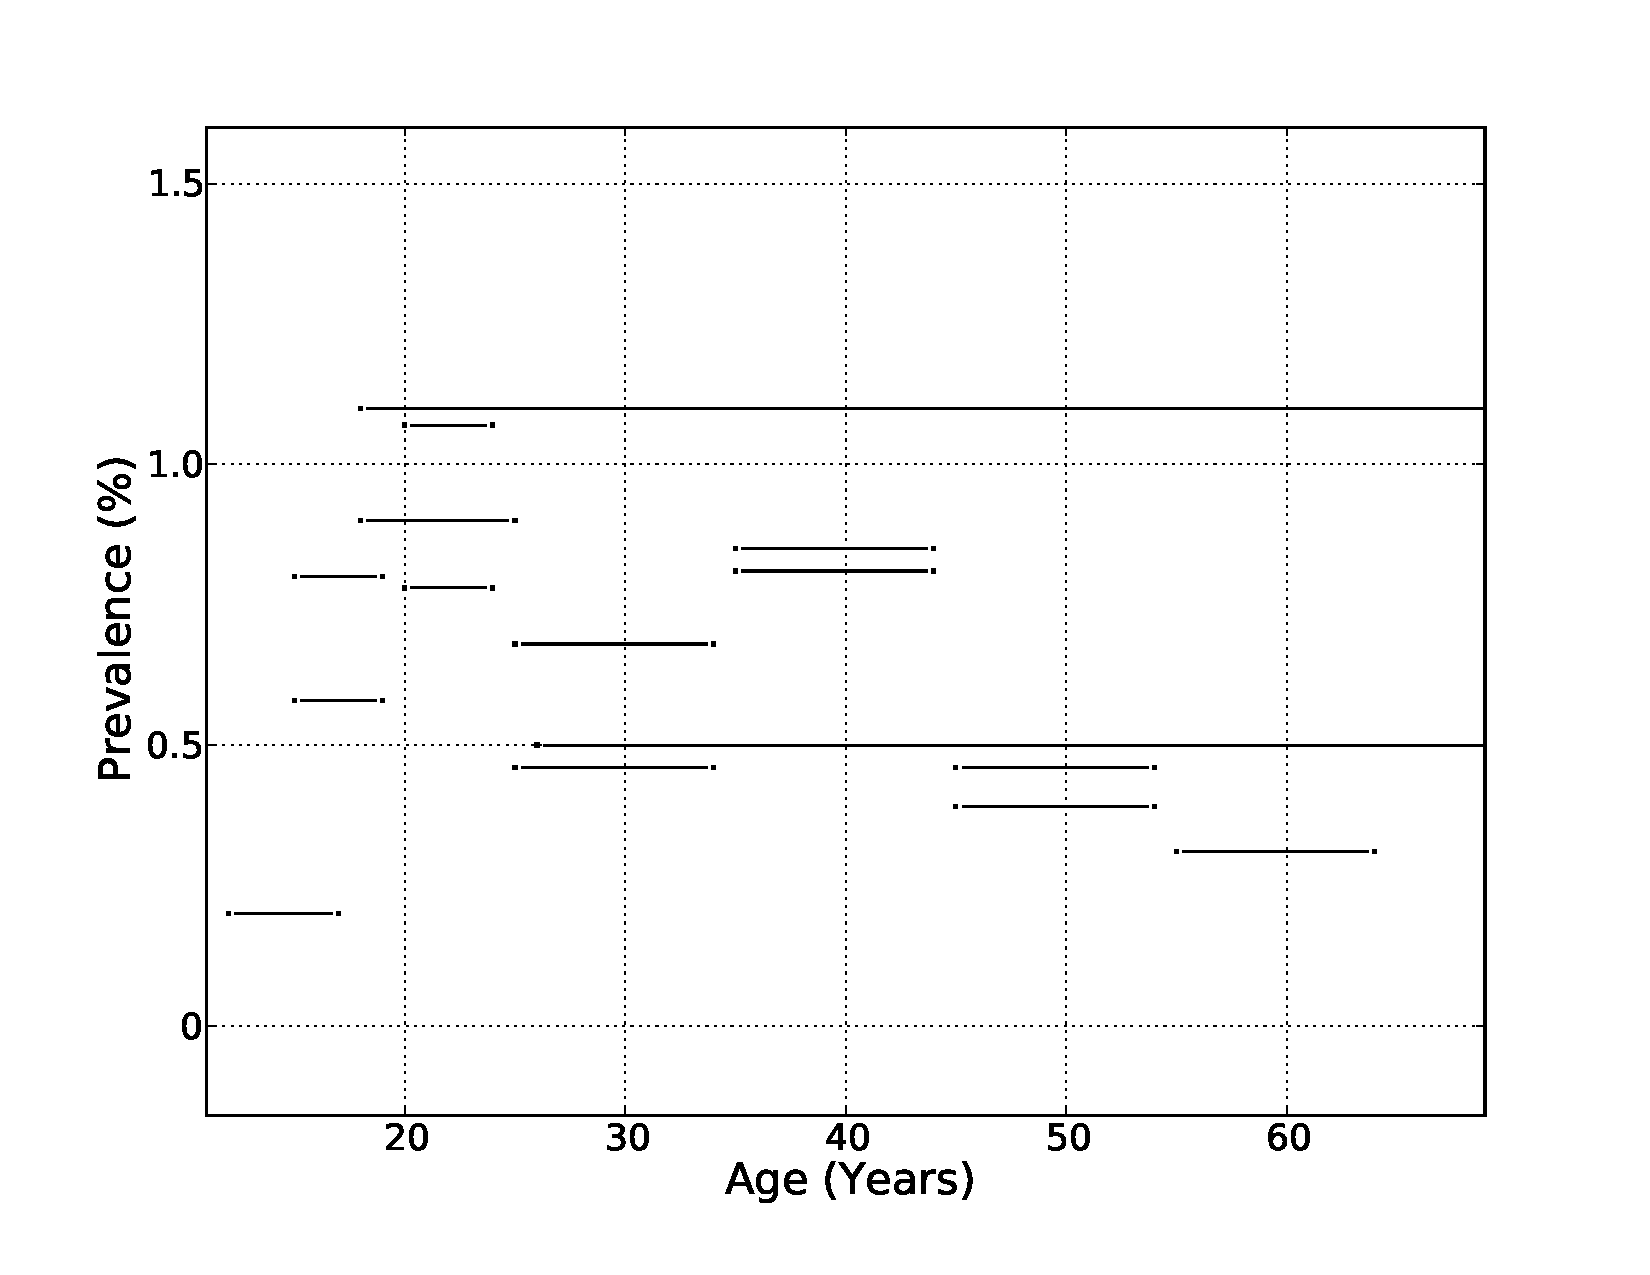
\includegraphics[width=\textwidth]{cocaine_dependence-data.pdf}
            \caption{Prevalence data for cocaine dependence in the
              United States of America. Each horizontal bar represents
              a single data point extracted in systematic review.  The
              left and right endpoints indicate the start and end ages
              of the age interval for a data point, while the level of
              prevalence is represented by the distance of the bar
              above the $y$-axis.}
            \label{fig:app-cocaine_data}
        \end{center}
    \end{figure}

As discussed in Chapter \ref{theory-age_pattern_model}, we model
age-specific hazards with spline models.  To be more specific, in this
case, the spline model takes the form of a continuous, piecewise
linear function, with ``knots'' where the function is non-linear
selected as part of the model.  These knots partition the age range
into intervals, and the choice of knots can be influential on the
resulting estimates.  In a setting where data is \emph{not} sparse and
noisy, estimates will not be very sensitive to choice of knots.
However, when working with sparse and noisy data, the number and
location of knots are important decisions as they can influence the
model results substantially.  Thus, the number of knots and locations
should be chosen a priori using expert knowledge concerning the
disease being modeled.  It is also
important to consider additional knots and alternative configurations
of knots as a sensitivity analysis.

To demonstrate the importance of the number of knots in a spline
model, three models with differing numbers of knots are compared in
Figure \ref{fig:app-cocaine_knots}.  The original model for cocaine
dependence had knot set $\{15, 20, 25, 30, 40, 50, 65\}$, based on the theory that prevalence is zero in childhood,
changes rapidly during early adulthood, and then changes less rapidly
in older ages.  The age pattern of prevalence estimated with this
model is shown as a solid line.

A model with less knots, using the knot set $\{15, 25, 40, 65\}$,
was also fit.  The estimates from this model, shown as a dotted line,
show how, seemingly paradoxically, fewer knots can lead to more
extreme estimates for certain ages.

A model with more knots, using knots spaced every five years from
ages 15 to 65, was also fit.
The estimates from this model are shown as a dashed line in
Figure~\ref{fig:app-cocaine_knots}.  When data is sparse, adding
additional knots allows for estimates that follow the vagaries of the
data more closely, which may not be desired.  Smoothing priors for the
penalized spline model can address this, which will be examined next.

    \begin{figure}[h]
        \begin{center}
            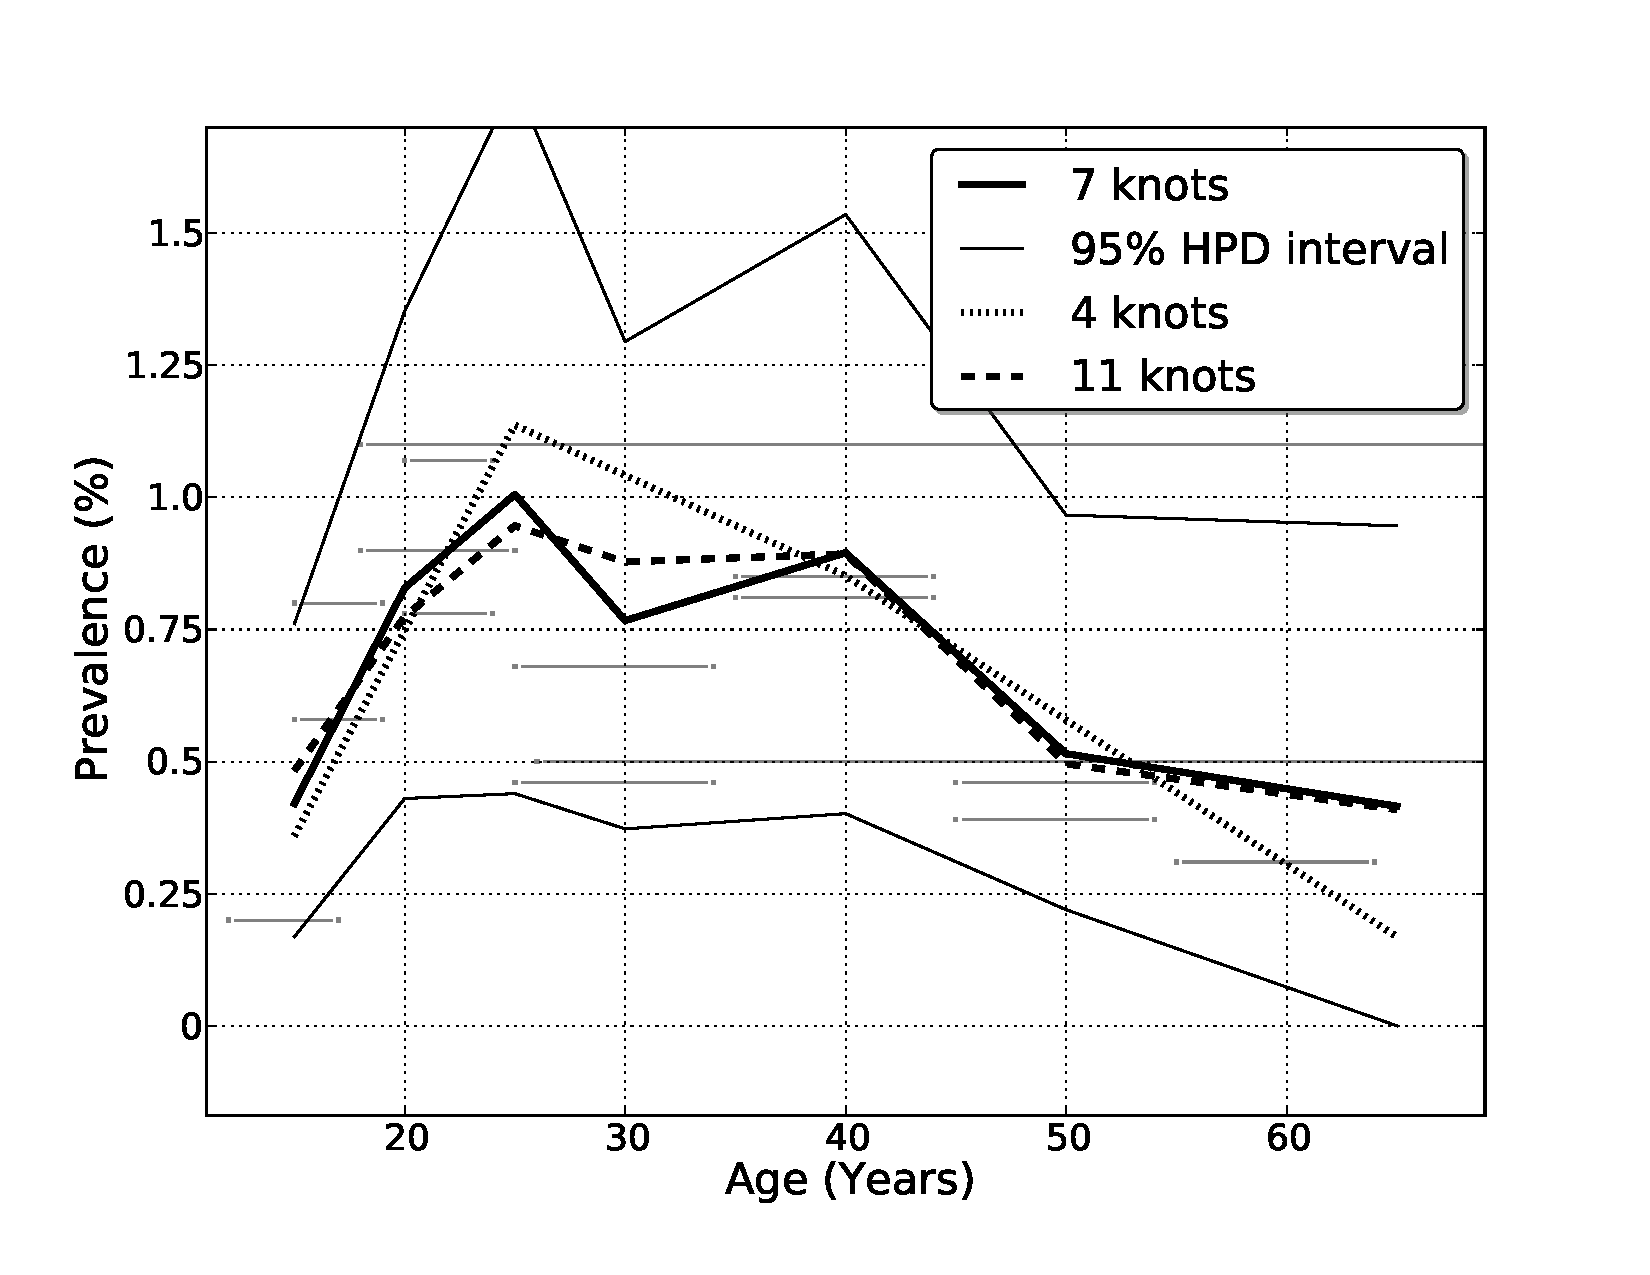
\includegraphics[width=\textwidth]{applications/cocaine_dependence-knots.pdf}
            \caption{Prevalence estimates of cocaine dependence in the United
              States of America using a spline model in the original
              model and models with less and more knots. }
        \label{fig:app-cocaine_knots}
        \end{center}
    \end{figure}

The penalized spline model introduces an additional term to the model
prior to encode the belief that the age pattern is not too wiggly.
With the judicious choice of the smoothness hyperparameter, the model
can include more knots without using them to chase the noise around in
the noisy data.  The effects of three values of smoothing parameter
are shown in Figure \ref{fig:app-cocaine_smoothing}.  The smaller the
parameter, the smoother the estimated age pattern, and hence the less
influential the position of the knots.  However, too much smoothing
leads to overcompression of the prevalence estimates with estimates
that are not representative of the data.

    \begin{figure}[h]
        \begin{center}
            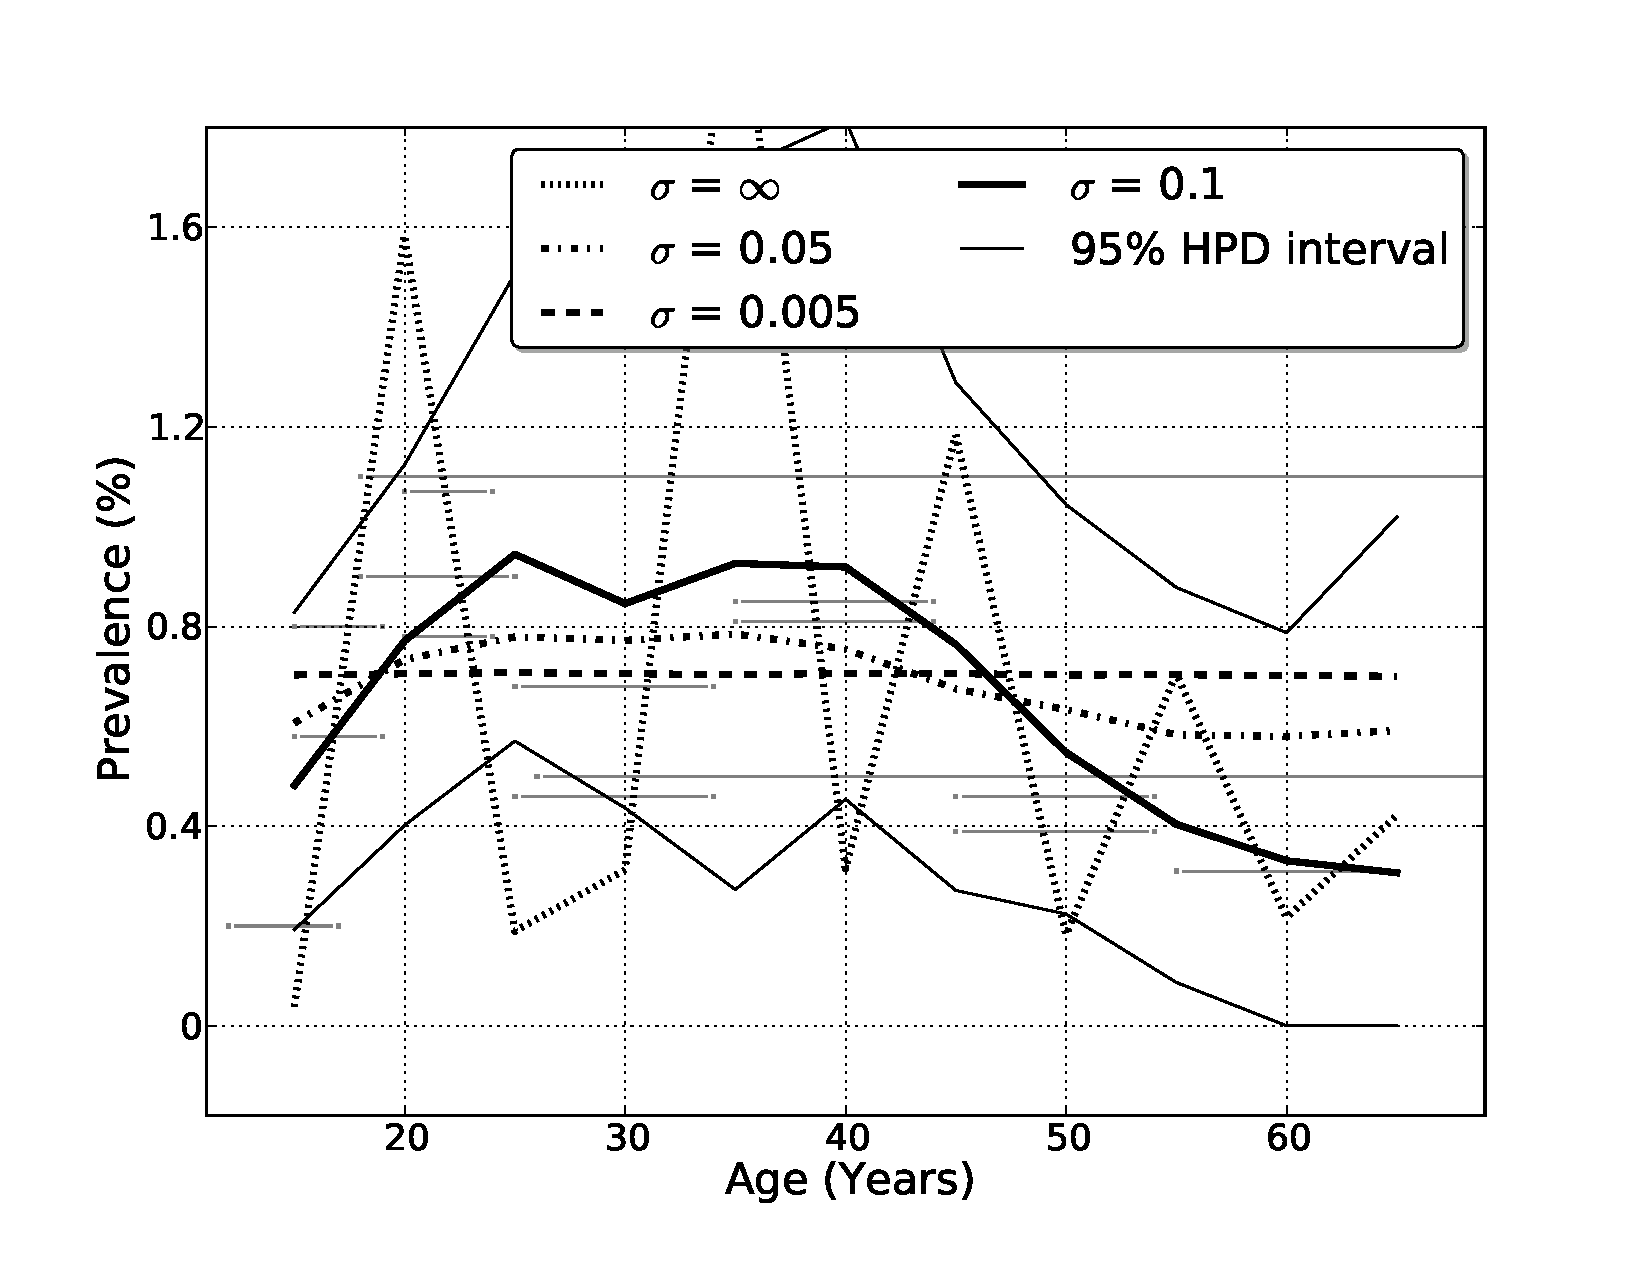
\includegraphics[width=\textwidth]{applications/cocaine_dependence-smoothing.pdf}
            \caption{Prevalence estimates from the model with knots every five years
              using a penalized spline model with a smoothing
              parameter $\sigma$. }
        \label{fig:app-cocaine_smoothing}
        \end{center}
    \end{figure}

As shown by the figures above, knot location and smoothing
hyperparameter selection can be an influential part of the model.
From the sensitivity analysis in Figure \ref{fig:app-cocaine_knots},
it appears that there is not anything to gain from adding additional
knots to the model, although it is possible to do so if an appropriate
smoothing parameter is included also.  In the next chapter, we will
consider a case where the data does not have such a clear story to
tell about the age pattern.

\chapter{Unclear age pattern, requiring expert priors: premenstrual syndrome}
\label{applications-priors_knots_select}

Epidemiological data without clear age patterns are a reoccurring
theme in the GBD 2010 Study.  Unclear age patterns make expert priors
essential in the modeling process.  However, such cases are very
sensitive to the choice of prior assumptions, as shown in the
following example of premenstrual syndrome (PMS) in Western Europe.

PMS is a common cyclic disorder that affects women of reproductive
years during the period between ovulation and the onset of menses.
More than $200$ behavioral, psychological, and physical symptoms have been
associated with PMS, the most common being irritability, tension,
depression, bloating, weight gain, and food cravings.  The exact causes
of PMS are unknown, with no consistent
treatment option available. \cite{dickerson_premenstrual_2003, singh_incidence_1998,
  goodale_alleviation_1990}

A meta-analysis of data from a systematic review of the descriptive
epidemiology of PMS yielded $74$ prevalence
data points, of which $18$ were from Western Europe.  As seen from
figure~\ref{fig:app-pms_data}, the data are noisy, with overlapping and
heterogeneous age-groups that show no clear age pattern.

    \begin{figure}[h]
        \begin{center}
            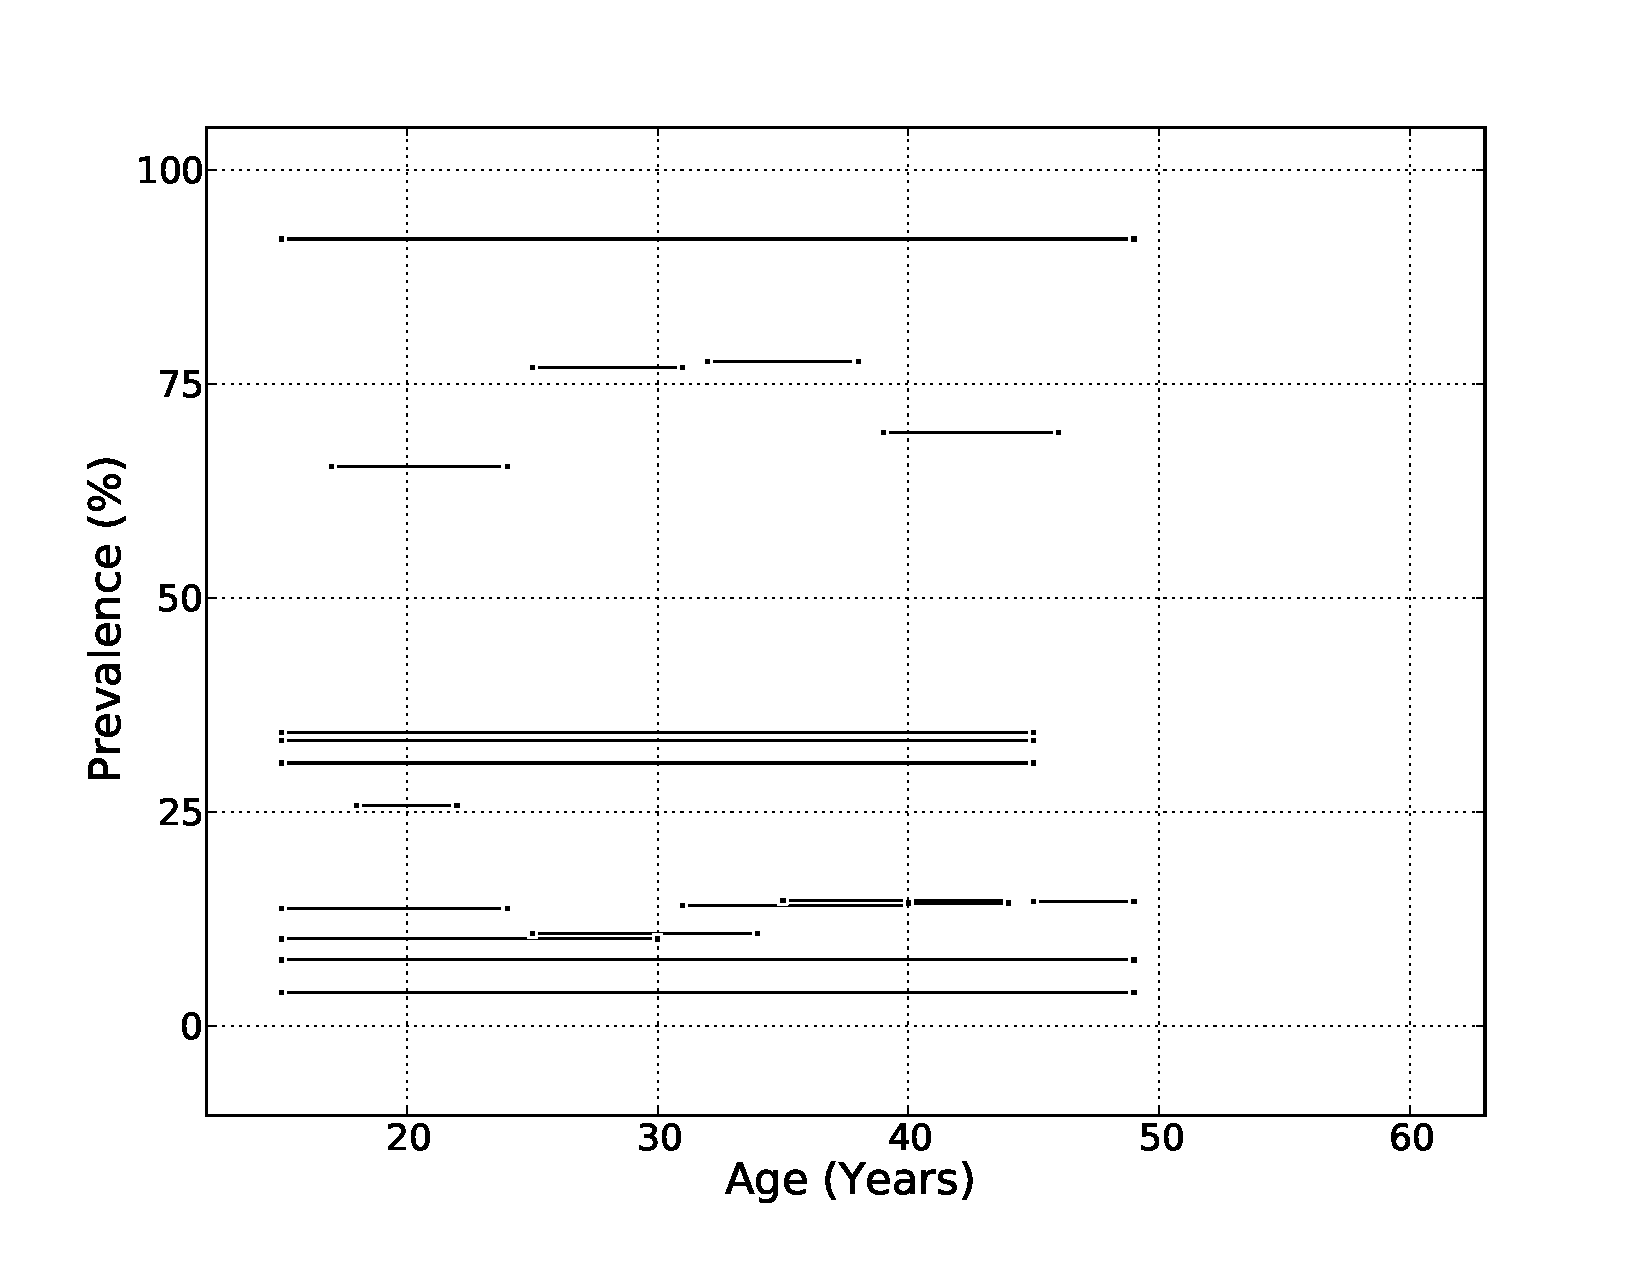
\includegraphics[width=\textwidth]{pms-data.pdf}
        \end{center}
        \caption{Prevalence data for women with PMS
              in Western Europe.}
        \label{fig:app-pms_data}
    \end{figure}

%% \section{Priors on level} \label{sec:app-priors on level}

In the absence of clear age patterns in the systematic review data
points, modeling decisions about knot location, age pattern levels, and
direction of age pattern trends have substantial influence on the estimates of
disease prevalence.  These decisions can also have unintended
consequences, as discussed in chapter~\ref{theory-age_pattern_model}.
To illustrate the effects, we fitted models with a variety of choices
about knot location, level values outside the measured age
intervals, and direction of age pattern trends.  Conducting a sensitivity analysis
like this is important when modeling sparse and noisy data.

As the prevalence data plotted in figure~\ref{fig:app-pms_data} show,
systematic review collected no data on population prevalence for women
younger than age $15$ or older than age $50$.  Since PMS is a disorder
related to the female reproductive cycle, it follows that data outside
this age range are not present for biological reasons.  However, this
information is not part of the spline model unless the modeler
explicitly includes it.  If no priors are included to inform estimates
in the young and old, then they are extrapolated from the levels where
there are data, as seen in figure~\ref{fig:app-pms prios_on_level}.
Here expert knowledge is needed to inform the model that cases are not
expected outside the age range where they have been measured.

    \begin{figure}
        \begin{center}
            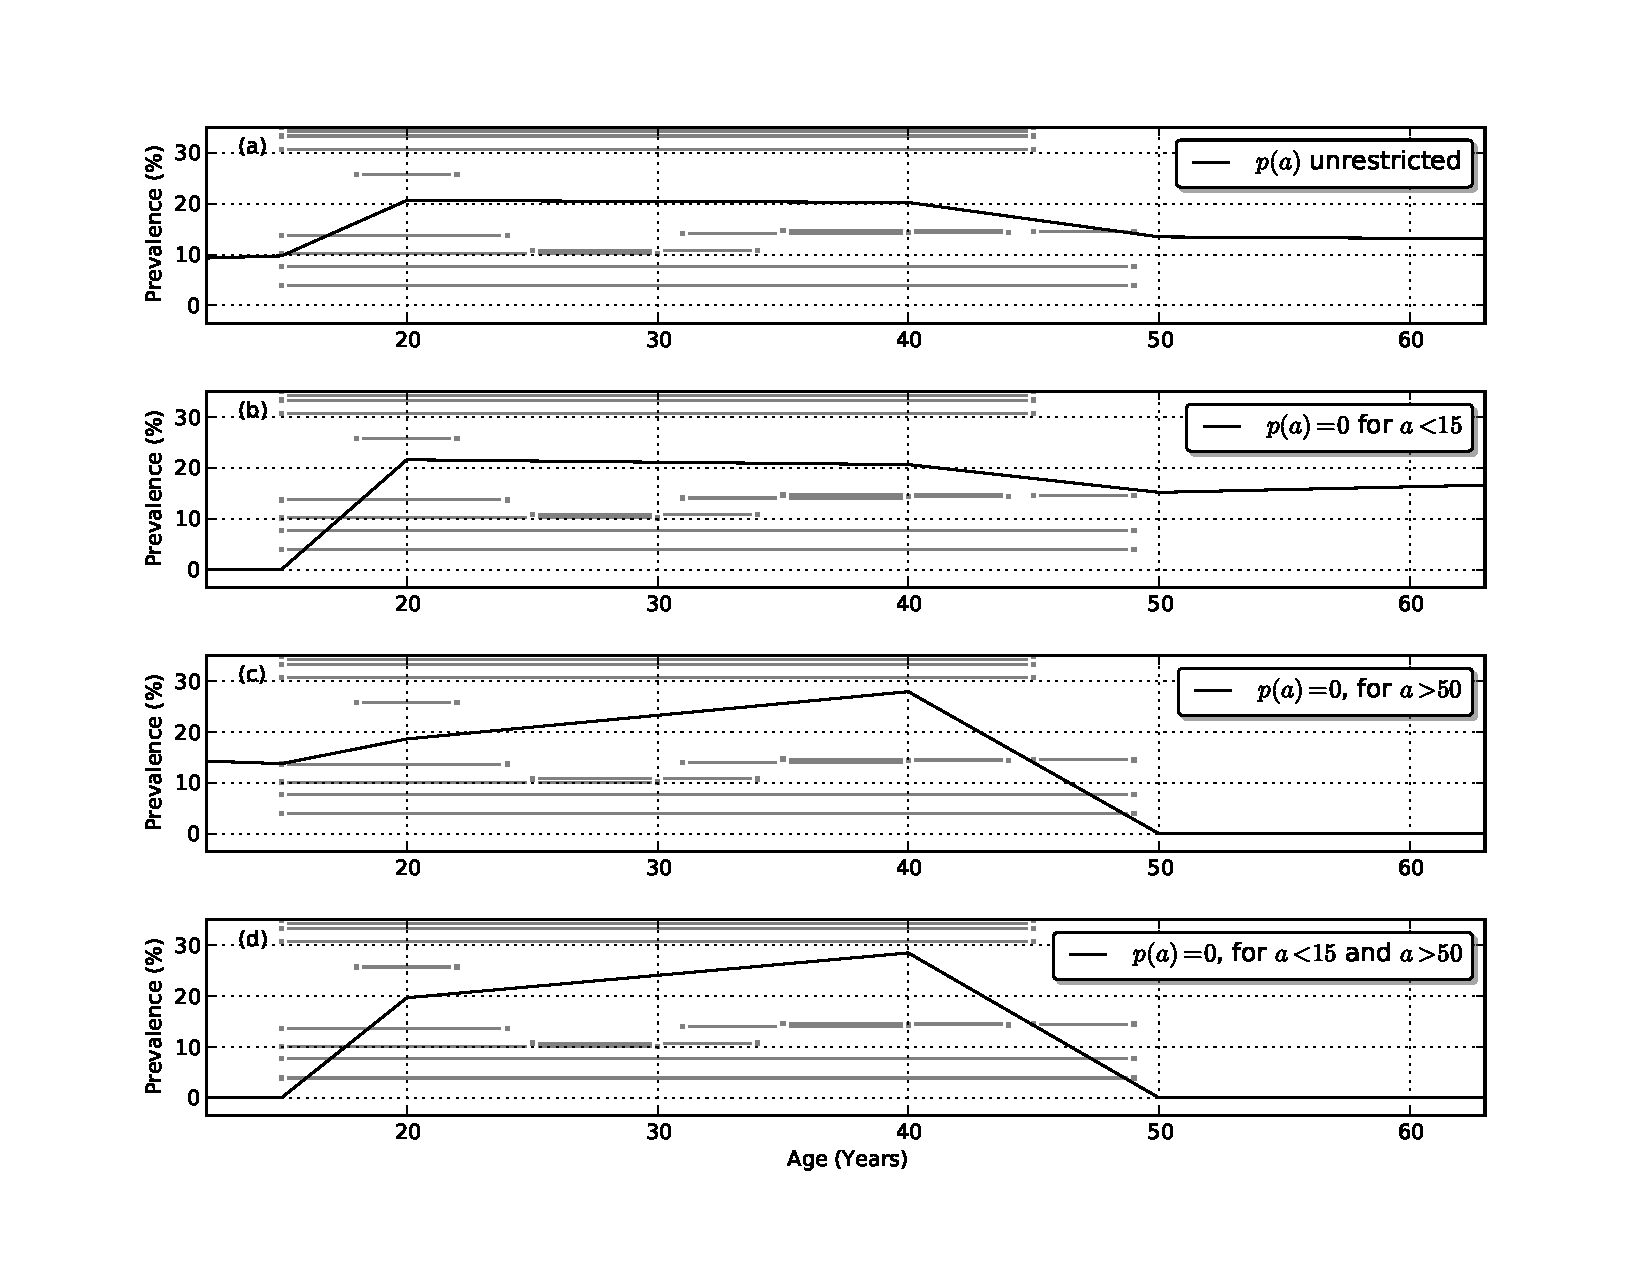
\includegraphics[width=\textwidth]{pms-priors.pdf}
        \end{center}
        \caption[Four estimates of age-specific PMS prevalence with
          different priors on prevalence in young and old ages]{Four
          estimates of age-specific PMS prevalence with different
          priors on prevalence in young and old ages.  Systematic
          review produced sparse and noisy data, shown here for
          Western Europe.  (a) Without a level prior to inform the
          model that prevalence data are not present outside
          ages $15$--$50$ for biological reasons, estimates outside the
          ages measured are extrapolated from inside.  Restricting
          prevalence to $0$ changes the prevalence estimates
          substantially. (b) The effect of assuming $p(a) = 0$ for
          $a<15$, (c) the effect of assuming $p(a) = 0$ for $a>50$,
          and (d) the effect of assuming $p(a) = 0$ for $a<15$ and
          $a>50$ all change the estimates inside and outside the
          observed data ages.}
        \label{fig:app-pms prios_on_level}
    \end{figure}

%% \section{Knot location}

As described in
section~\ref{spline_models}, we model
age-specific hazards with splines, using knots to partition the age
range into intervals.  Models with ample data and clear age patterns
are not very sensitive to knot choice.  However, with sparse and
noisy data without a clear age pattern, the number and location of
knots can influence the model results substantially.  We explored this
by fitting models with a variety of knots to the PMS data set, as seen
in figure~\ref{fig:app-pms knot_loc}.  Choosing the number and
location of knots a priori using expert knowledge allows the user to
determine critical features of the model in a principled way.

    \begin{figure}
        \begin{center}
            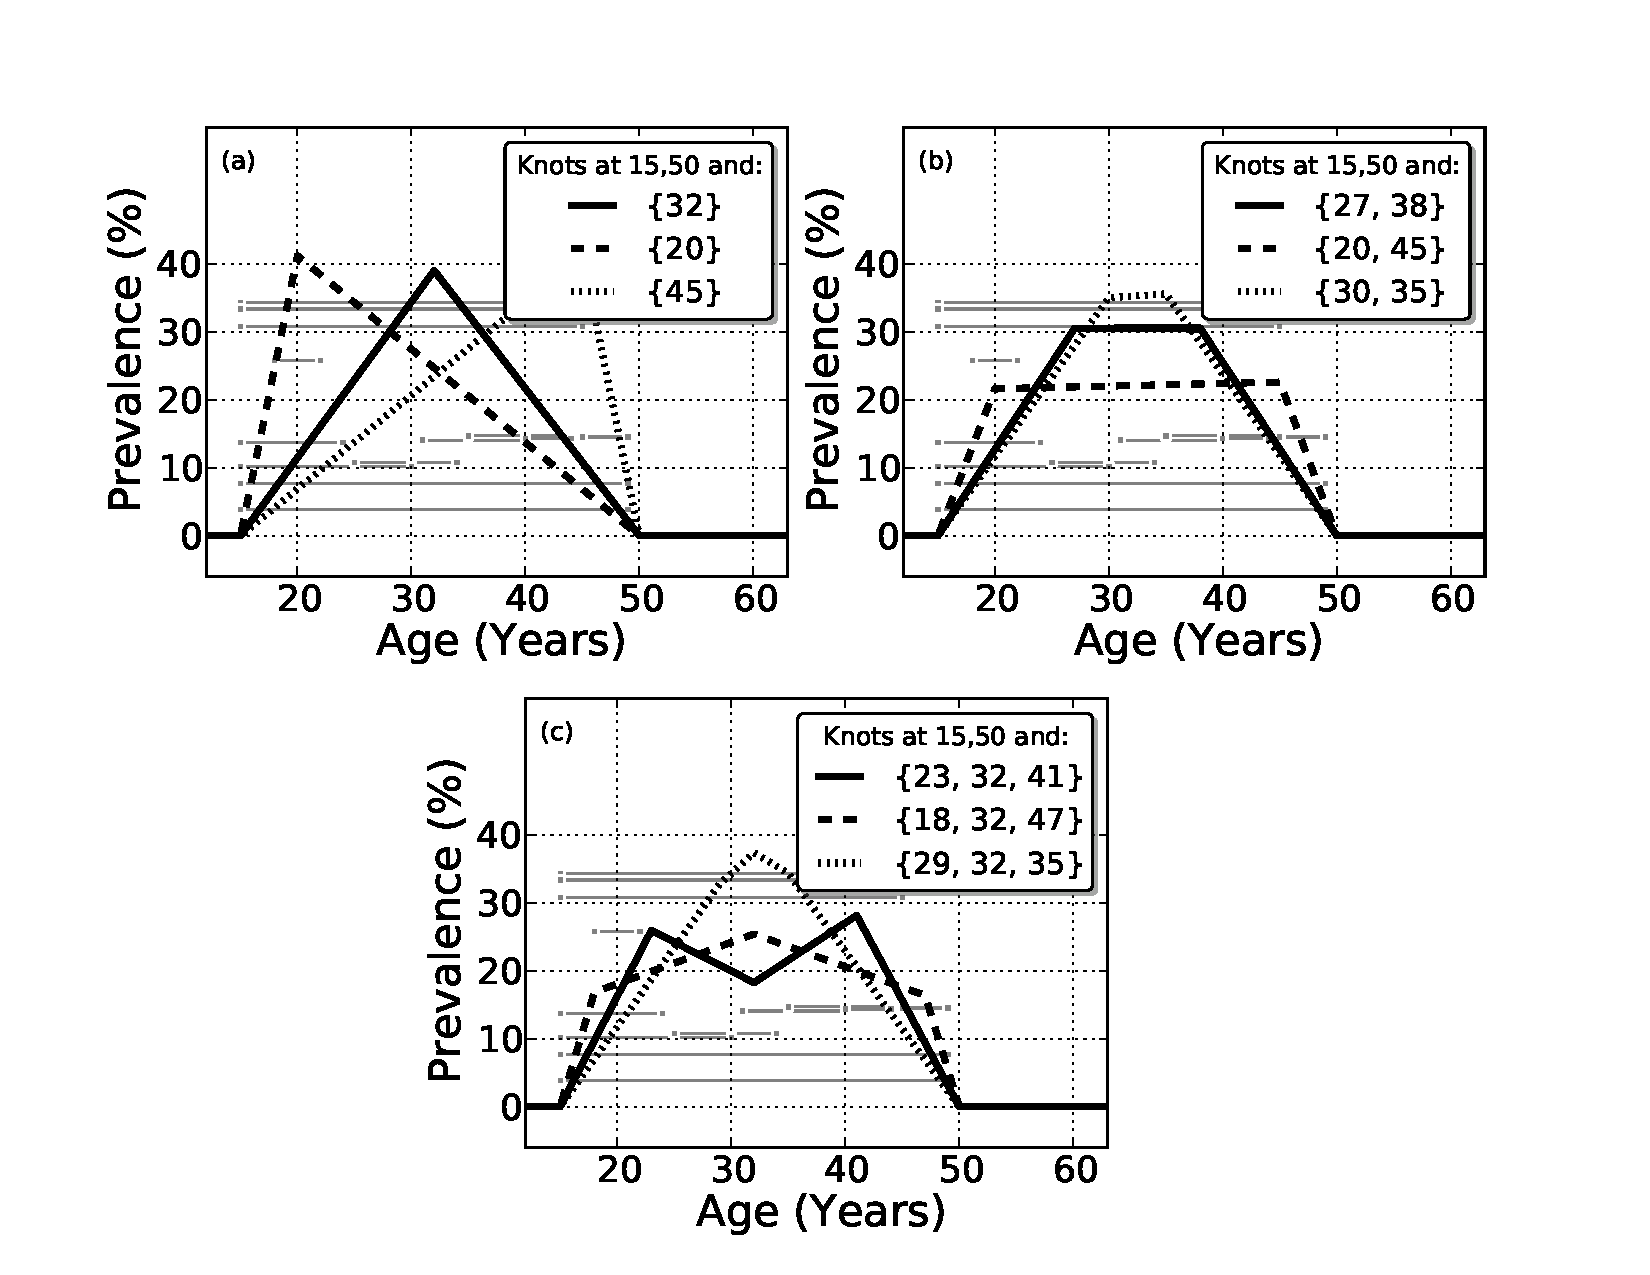
\includegraphics[width=\textwidth]{pms-knot_location.pdf}
        \end{center}
        \caption[Estimate of age-specific PMS prevalence for spline
          models with a variety of knots]{Estimate of age-specific PMS
          prevalence for spline models with a variety of knots.  All
          panels have knots at $\{0, 15, 50, 100\}$ and vary the number
          and location of knots between the ages of $15$ and $50$ to show
          the sensitivity of knot selection in sparse and noisy data
          without a clear age pattern. (a) With $1$ additional knot, the
          placement at age $20$, $32$, or $45$ gives markedly different
          estimates of PMS prevalence in Western Europe.  (b) With $2$
          knots at $\{27, 38\}$, $\{20, 45\}$, or $\{30, 35\}$, the
          differences are also clear and predictable. (c) With $3$ knots
          at locations $\{23, 32, 41\}$, $\{18, 32, 47\}$, or $\{29, 32,
          35\}$, it appears that the data are too sparse and noisy to
          support a consistent age pattern.}
        \label{fig:app-pms knot_loc}
    \end{figure}

%% \section{Priors on monotonicity}
Another common prior for age patterns is the belief that the
epidemiological parameter increases or decreases over a certain age
range.  As seen in figure~\ref{fig:app-pms dir}, priors on
monotonicity between the critical ages of $25$ and $40$ have a large
effect on the prevalence estimate for Western Europe.

    \begin{figure}
        \begin{center}
            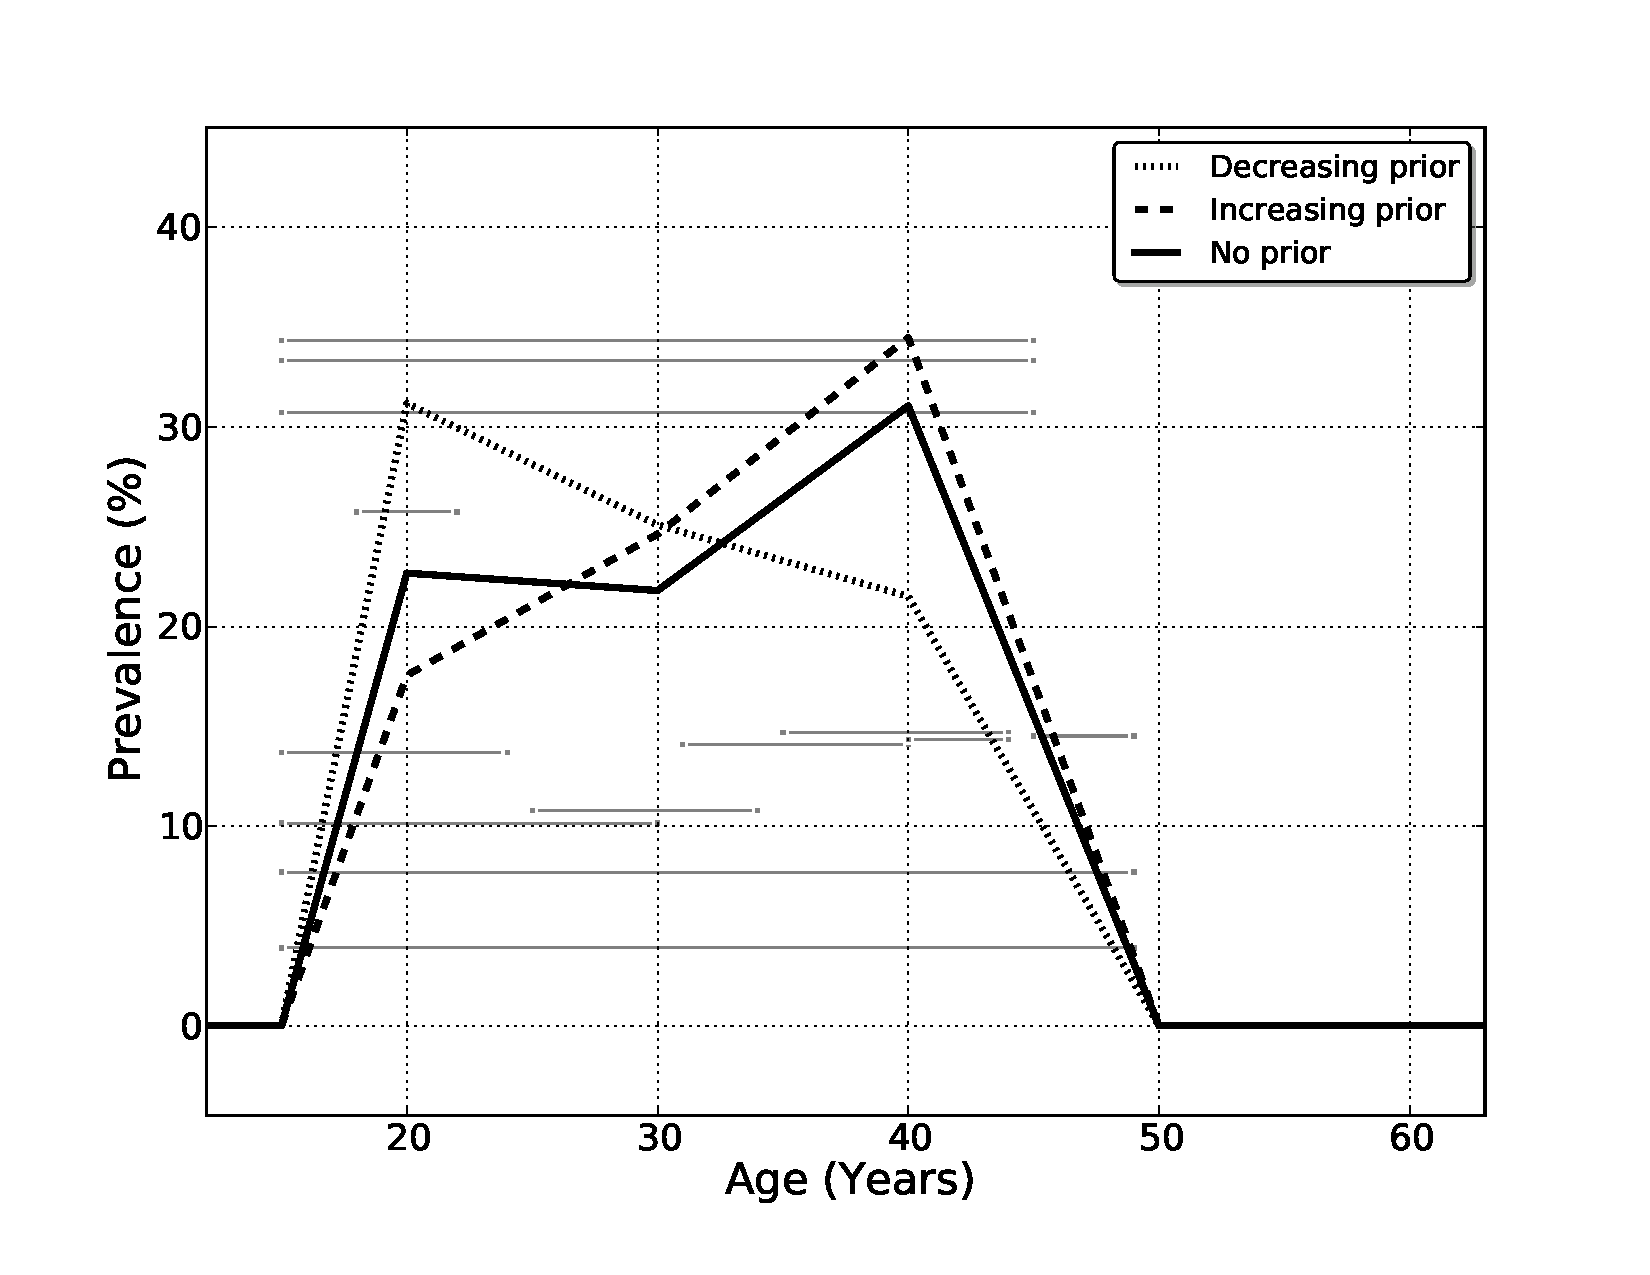
\includegraphics[width=\textwidth]{pms-direction.pdf}
        \end{center}
        \caption[Estimates of age-specific PMS prevalence for spline
          models with a variety of monotonicity priors]{Estimates of
          age-specific PMS prevalence for spline models with a variety
          of monotonicity priors. Between the ages of $25$ and $40$, the prior
          on monotonicity makes a large impact on the prevalence
          estimates for women in Western Europe with PMS.}
        \label{fig:app-pms dir}
    \end{figure}

Knot selection and priors on level and monotonicity play an important
role in the modeling process and in the sensitivity analysis.
However, when the data are not sufficient to understand the age
pattern, the model compensates by producing estimates with large
uncertainty, as seen in figure~\ref{fig:app-pms best}.  This estimate
comes from a model with knots at $\{0, 15, 20, 30, 40, 50, 100\}$, no
prior on monotonicity, and a prior on level to restrict prevalence to
be $0$ outside the age range $15$--$50$.

This example has identified an area of future research.  The model does
not have enough data to inform an age pattern because the descriptive
epidemiology of PMS is quite uncertain: some studies say almost all women
experience it and some studies say none do.  In such cases, making the
most informed decisions possible (such as restricting the model to
ages $15$--$50$ for biological reasons) and accepting a large uncertainty
interval reveal the truth: we just don't know.

    \begin{figure}
        \begin{center}
            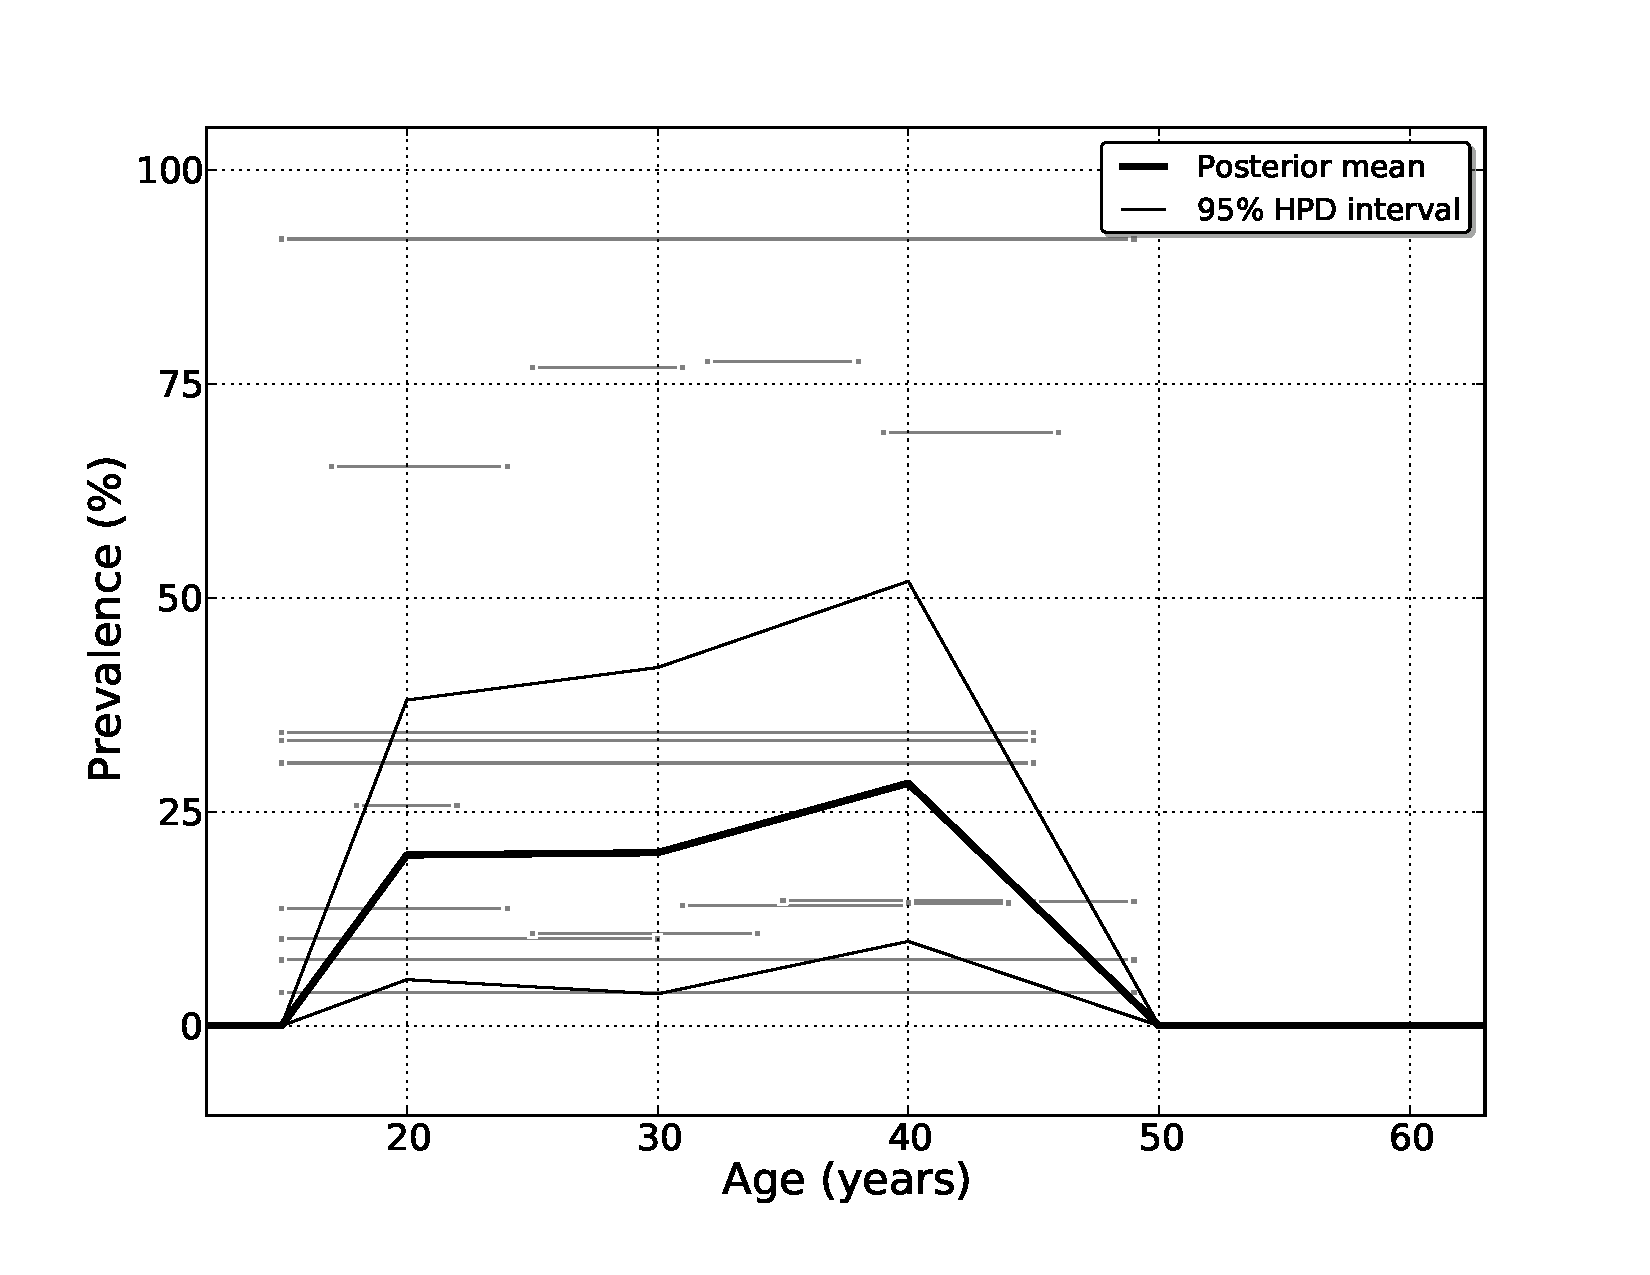
\includegraphics[width=\textwidth]{pms-best_model.pdf}
        \end{center}
        \caption{Prevalence estimates for women
          in Western Europe with PMS.}
        \label{fig:app-pms best}
    \end{figure}










\chapter{Dealing with geographical variation: hepatitis C}
\label{applications-rfx}

Hepatitis C is a viral infection that attacks the liver.  In a small
portion of acute cases, the body can eliminate the virus; however the
majority of acute cases develop into chronic infections.  Chronic
infections cause liver damage and may develop into end stage liver
disease or cirrhosis.  Few, if any, chronic cases experience symptoms
and only one third of acute cases are symptomatic and jaundice.
Chronic symptoms are nonspecific, intermittent and mild with the most
common symptom being fatigue.  Common symptoms for severe and advanced
disease stages include nausea, dark urine and jaundice.  Since
hepatitis C infections are asymptomatic, diagnosis requires laboratory
testing for both hepatitis antibodies (anti-HCV) and the hepatitis
virus (HCV RNA).  There is no vaccination for hepatitis C, but therapy
can prevent advanced liver disease. \cite{hoofnagle_hepatitis_1997,
  ghany_diagnosis_2009}

Compared to other countries in the region, Egypt has a high hepatitis
C prevalence.  In an attempt to treat endemic schistosomiasis, a
common parasitic worm that affects the urinary tract, gut and liver,
the Egyptian Ministry of Health launched widespread injection-based
treatment throughout 1950-1980.  While there were improvements in
schistosomiasis-induced mortality, recycled needles and poor needle
sterilization infected many with hepatitis C. \cite{frank_role_2000,
  mezban_hepatitis_2006, strickland_liver_2006} The spatial variations
of hepatitis C in North Africa and the Middle East make it an
excellent example for hierarchical random effects modeling.

Random effects modeling detects systematic differences among different
hierarchies, or levels, of data.  The spatial hierarchy in the GBD
2010 study uses countries nested in regions nested in super-regions.
There are 21 regions defined by demographic and epidemiological
similarities that are further clustered by 7 super-regions.

The analysis of hepatitis C uses data on the prevalence of persons who
have hepatitis C antibodies.  Incomplete data or data from high-risk
populations, such as health care workers, were excluded.  Notice that
hepatitis C prevalence in Egypt is more than 40 times that of the
Jordan, even though they are both in the region of Northern Africa and
the Middle East (Figure \ref{fig:app-hepc data}).

    \begin{figure}[h]
        \begin{center}
            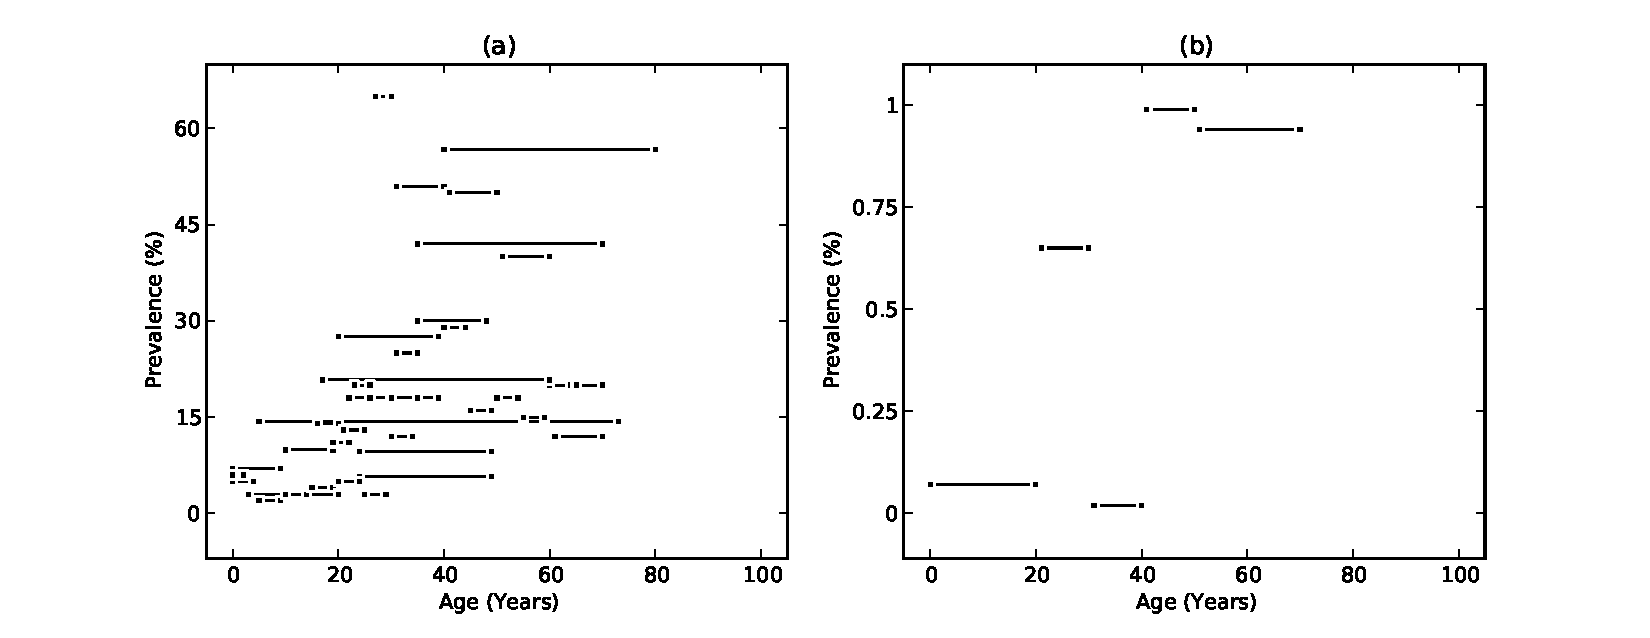
\includegraphics[width=\textwidth]{hepc-data_EGY_v_JOR.pdf}
            \caption{Prevalence data from systematic review of
              hepatitis C in Jordan (panel (a)) and Egypt (panel
              (b)).}
            \label{fig:app-hepc data}
        \end{center}
    \end{figure}

The analysis uses an age-standardizing hierarchical random effects
generalized negative binomial spline model to estimate prevalence.
The hierarchical random effects allow the model to capture variation
within the region of North Africa and the Middle East.  Looking at
Table \ref{tab:app-hepc regional rfx}, Egypt (EGY) has significantly
higher prevalence than the other countries in the region.  Figure
\ref{fig:app-hepc regional rfx} confirms this as the prevalence
estimate for Egypt is much above the regional average.

    \begin{table}[h]
        \begin{center}
        \caption{ Estimates of the intercept shift of hepatitis C prevalence in log space from a random effects model in the region of North Africa and the Middle East.}
        \label{tab:app-hepc regional rfx}
        \begin{tabular}{|c|c|c|c|}
            \hline
                Country & Posterior Mean & Lower 95\% HPD  & Upper 95\%  HPD \\
            \hline
                EGY	&	1.88	&	 1.6	&	2.2	\\
                JOR	&	-0.59	&	-1.1	&	-0.2 \\
                SAU	&	-0.78	&	-1.1	&	-0.4 \\
                IRQ	&	0.07	&	-0.4	&	0.6	\\
                IRN	&	0.00	&	-0.5	&	0.4	\\
                YEM	&	0.04	&	-0.3	&	0.4	\\
                TUR	&	-0.32	&	-0.7	&	0.0	\\
                SYR	&	-0.16	&	-0.6	&	0.4	\\
                TUN	&	-0.19	&	-0.7	&	0.3	\\
            \hline
        \end{tabular}
        \end{center}
    \end{table}

    \begin{figure}[h]
        \begin{center}
            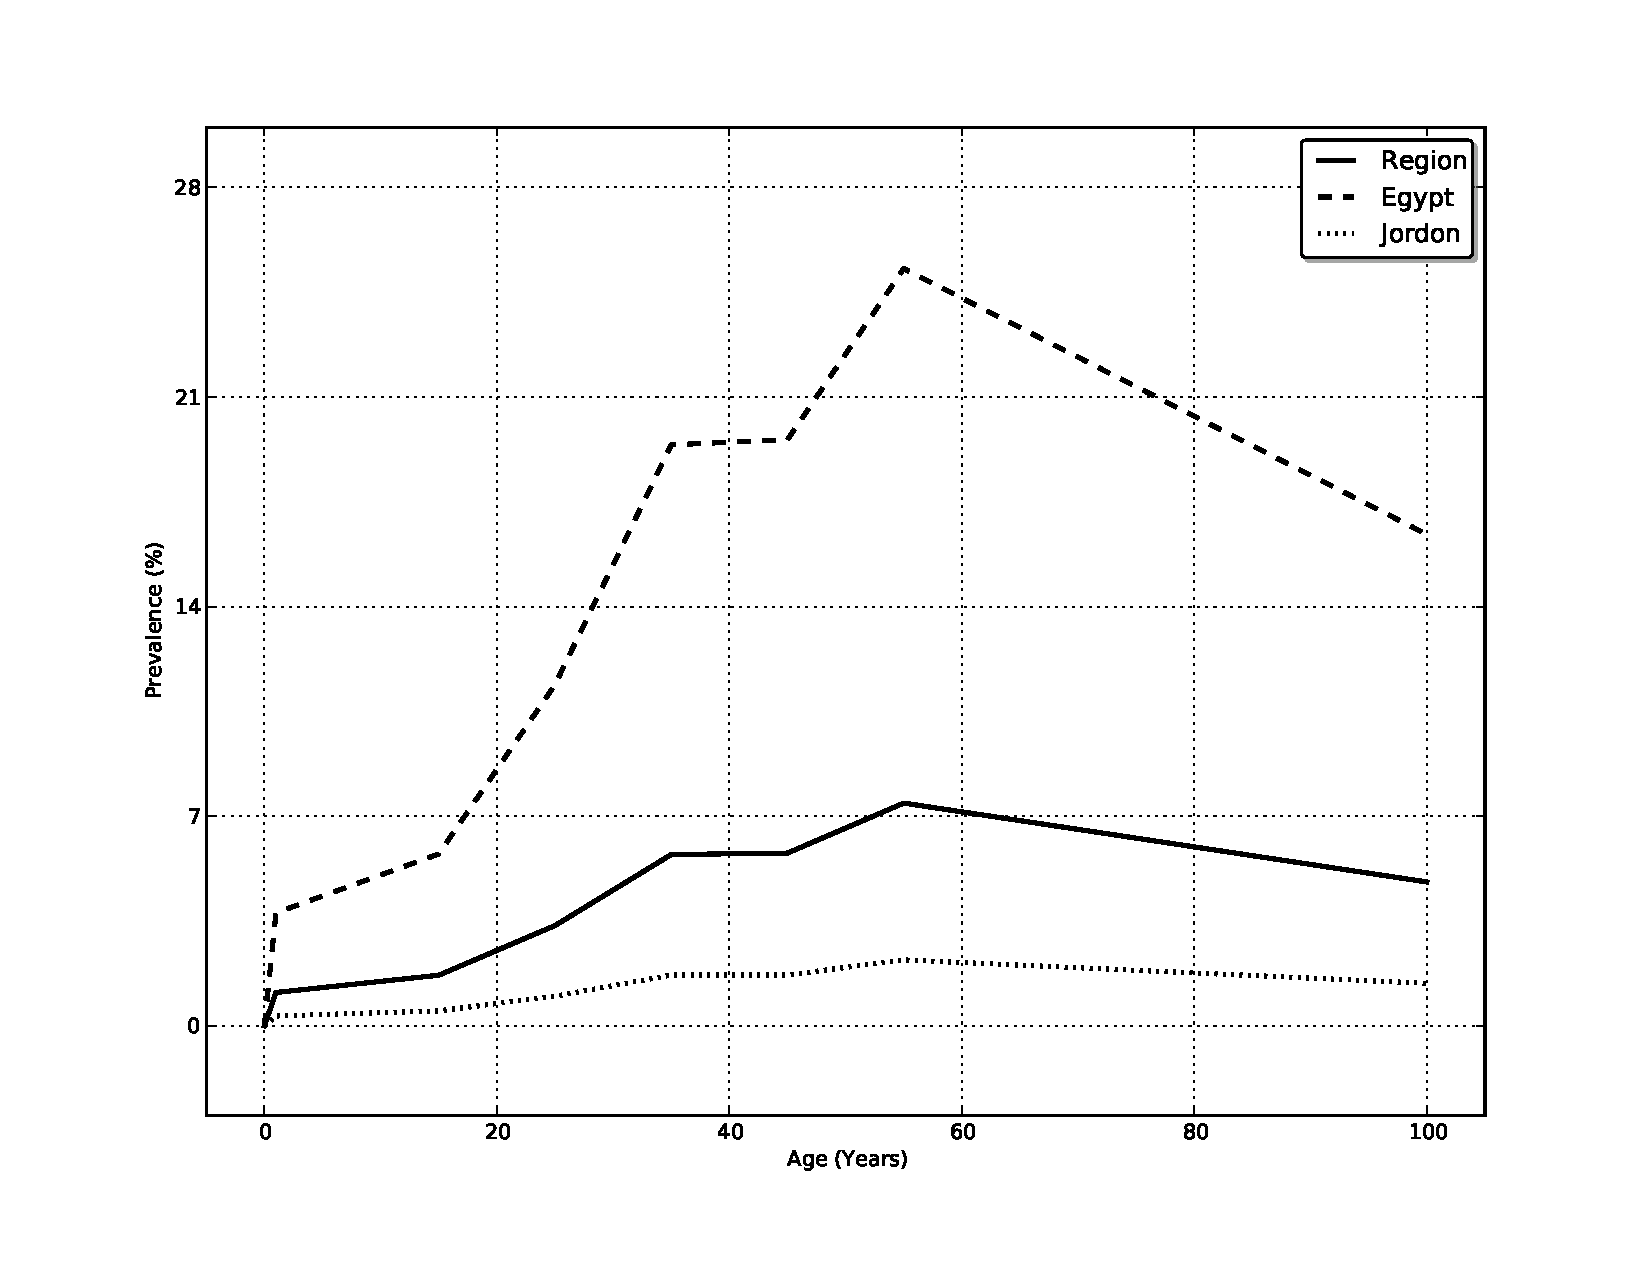
\includegraphics[width=\textwidth]{hepc-region_v_EGY_v_JOR.pdf}
            \caption{The 1990 estimate of hepatitis C prevalence for men in the region of North Africa and Middle East and the countries Egypt and Jordan.  These estimates only use 2 levels in the hierarchal random effects model--region and country.}
            \label{fig:app-hepc regional rfx}
        \end{center}
    \end{figure}

In such noisy data, placing a prior on the dispersion of the data
informs the model of the data heterogeneity.  This allows the model to
infer how dispersed the random effects are between geographic regions,
hence quantifying the uncertainty in the geographic regions for which
no data are available.  Priors on the dispersion parameter, $\delta$,
may be one of three categories, `very', `moderately' or `slightly'.
The natural logarithm of $\delta$ is uniformly distributed between its
lower and upper bounds.  Intended as a weakly informative prior, the
bounds of the categories overlap, so that the bounds of 'very' are
[1,9], 'moderately' are [3,27] and 'slightly' are [9,81].

In this example, the effects of priors on the overdispersion of
$\delta$ are seen in the posterior estimates at the country level as
seen in Figure \ref{fig:app-hepc global hetero}.  Random effects
modeling detects within sample variation and true variation that
cannot be explained by a covariate.  Therefore, a change in the prior
on global heterogeneity changes the level of variation and thus the
random effect size.  As seen in figure \ref{fig:app-hepc global
  hetero}, when the prior on global heterogeneity is `very', the
estimates are compressed.

    \begin{figure}[h]
        \begin{center}
            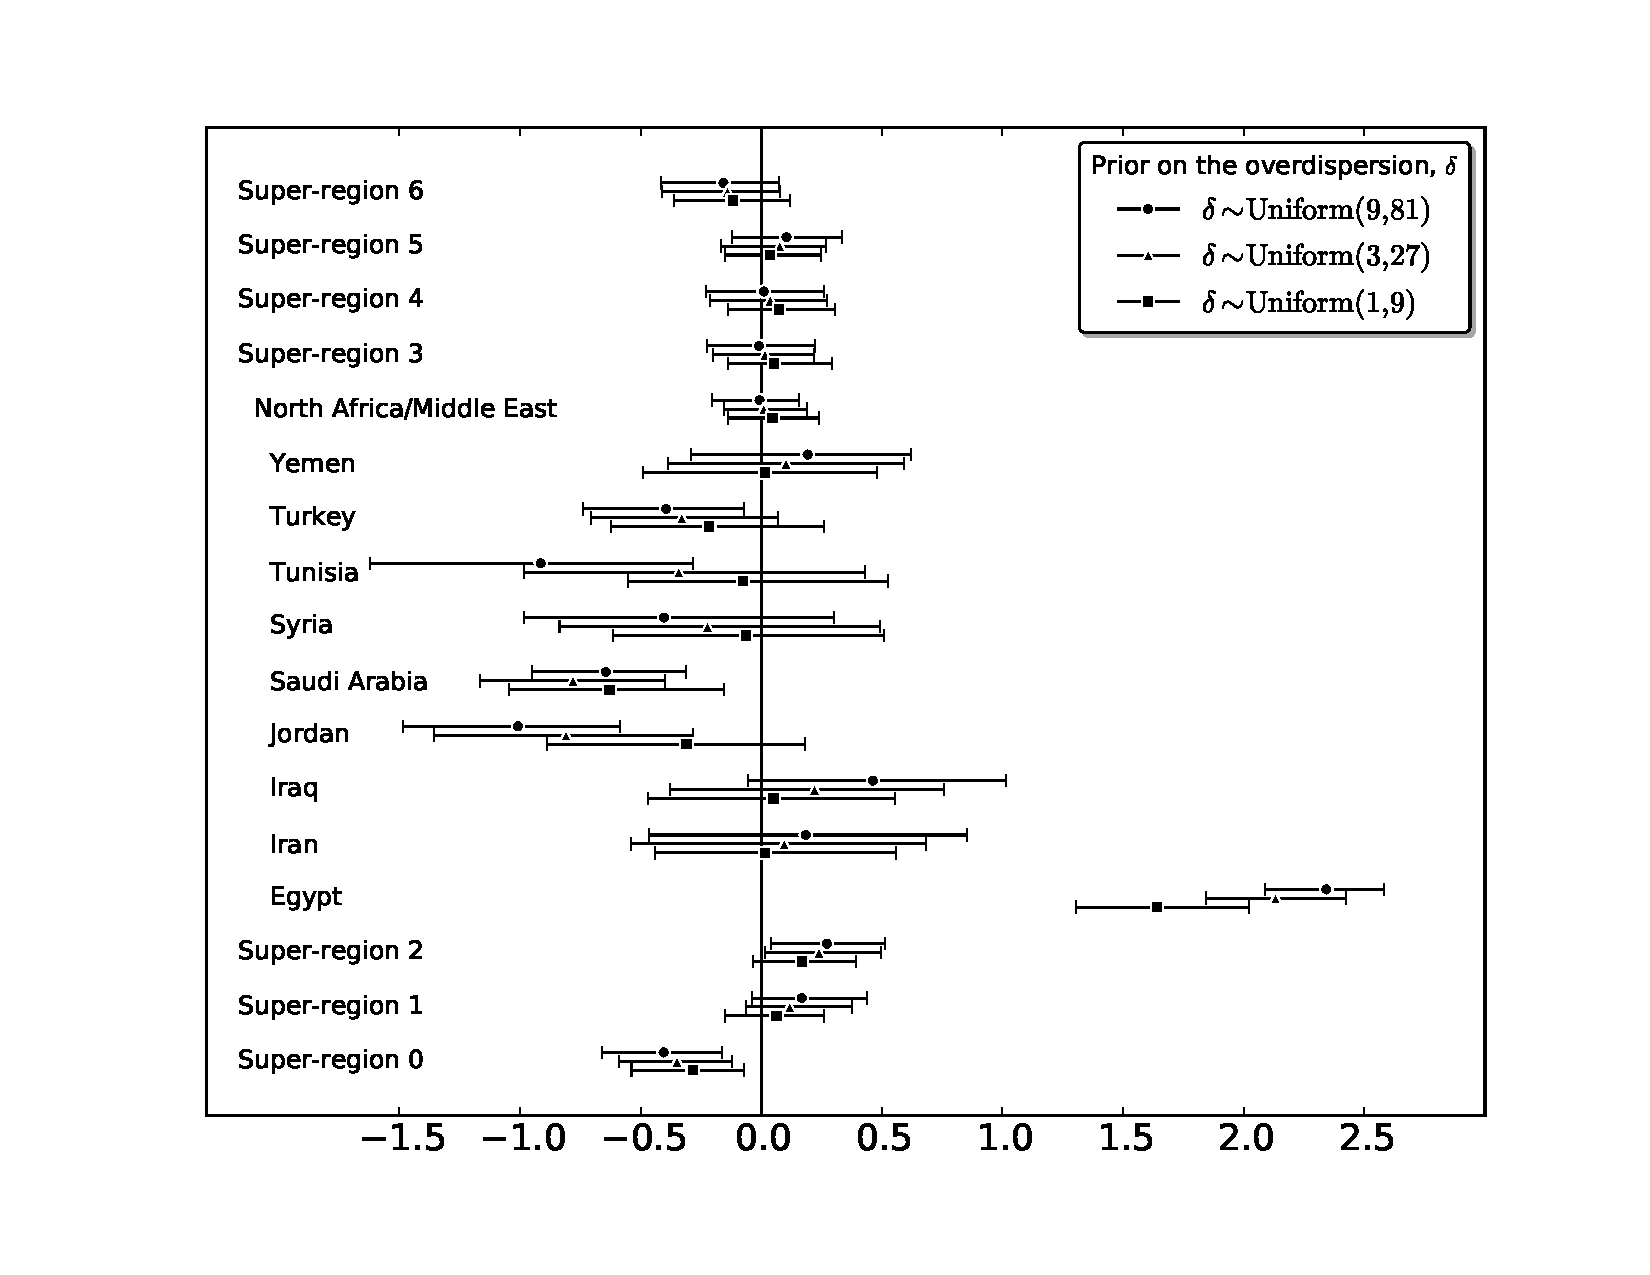
\includegraphics[width=\textwidth]{hepc-tree_plot_global_hetero.pdf}
            \caption{The 1990 intercept shift of hepatitis C
              prevalence in log space for men with different priors on
              global heterogeneity, $\delta$.  Four levels (global,
              super-region, region, country) were used in the
              hierarchal random effects model.}
            \label{fig:app-hepc global hetero}
        \end{center}
    \end{figure}

Another way to view compressed estimates is by looking at the
age-standardized prevalence in Table \ref{tab:app-hepc global rfx}.
As heterogeneity increases from `slightly' to `very', country
estimates are compressed toward the regional mean.

    \begin{table}[h]
        \begin{center}
        \caption{ Hepatitis C age-standardized prevalence estimates from a hierarchal random effects single rate type model with differing priors on global heterogeneity.}
        \label{tab:app-hepc global rfx}
        \begin{tabular}{|c|c|c|c|}
            \hline
                & & Posterior & Standard \\
                Geographic Area & Heterogeneity & Mean & Deviation \\
            \hline
                & $\delta \sim \Uniform(9,81)$ & 0.048 & 0.003 \\
                North Africa Middle East & $\delta \sim \Uniform(3,27)$ & 0.049 & 0.004 \\
                & $\delta \sim \Uniform(1,9)$ & 0.045 & 0.005 \\
            \hline
                & $\delta \sim \Uniform(9,81)$ & 0.007 & 0.002 \\
                Jordan & $\delta \sim \Uniform(3,27)$ & 0.010 & 0.003 \\
                & $\delta \sim \Uniform(1,9)$ & 0.020 & 0.006 \\
            \hline
                & $\delta \sim \Uniform(9,81)$ & 0.188 & 0.012 \\
                Egypt & $\delta \sim \Uniform(3,27)$ & 0.178 & 0.017 \\
                & $\delta \sim \Uniform(1,9)$ & 0.136 & 0.019 \\
            \hline
        \end{tabular}
        \end{center}
    \end{table}

\chapter{Cross-walking with fixed effects: anxiety disorders}
\label{applications-efx_study_level}

The data collected in systematic review often contain a variety of
different study types or diagnostic criteria, which create systematic
biases in the measured data.  An extreme example was found in the
systematic review of diabetes prevalence, where there were $18$ variants
of diagnostic criteria.  The systematic review of anxiety disorders
provides a simpler example, which is the focus of this chapter. This
systematic review collected studies that used a handful of different
recall periods to ask about the presence of the disorders. The quantity
of interest for estimation was point prevalence, the
proportion of the population with the condition at an instant in time.
We used a fixed-effect model to adjust for the bias introduced by
studies that measured period (e.g., past-year) prevalence, since these studies also provide
valuable information on the descriptive epidemiology of the condition.
This bias adjustment by fixed-effect modeling is also called a
``cross-walk.''

Anxiety disorders include at least $8$ separate conditions each
characterized by prominent anxiety at a level that interferes with
daily life.  Not all anxiety disorders manifest in similar ways.
While generalized anxiety disorder is typically marked by persistent
worry, panic disorder is usually characterized by intense fear for
discrete periods of time. \cite{american_psychiatric_association_diagnostic_2000} As there is
a lot of comorbidity between individual anxiety disorders, anxiety
disorders were modeled together as a single condition in the GBD 2010
Study.

Anxiety disorders do not have a consistent recall period for the
measurement of epidemiological rates.  Therefore, the data from
systematic review include studies with measurements of point prevalence
and period prevalence (i.e., $6$-month or past-year prevalence).  The
analysis excludes lifetime prevalence measurements because such estimates
are particularly prone to recall bias.  Due to the nonnegligible
remission rate for anxiety disorders, period prevalence is typically
higher than point prevalence, as seen in figure~\ref{fig:app-anxiety
  data}.

    \begin{figure}[h]
        \begin{center}
            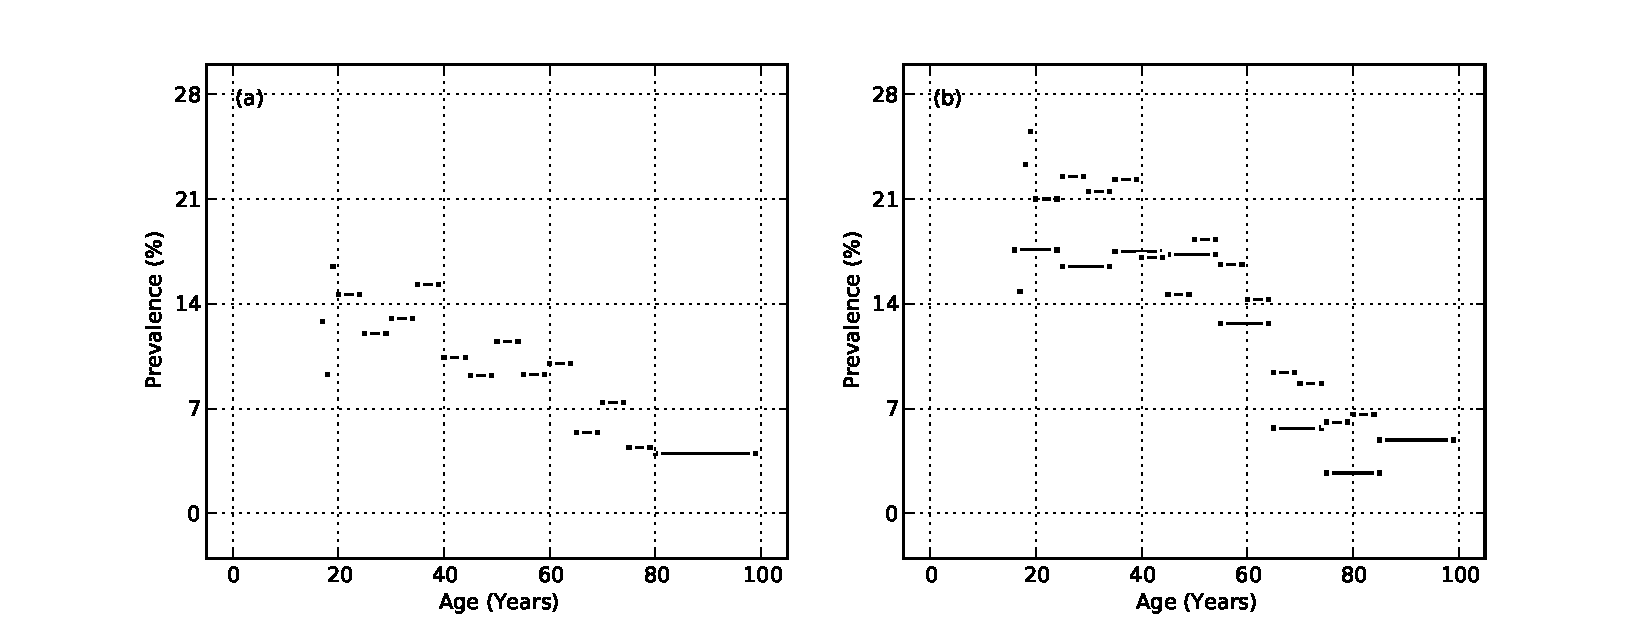
\includegraphics[width=\textwidth]{anxiety-data_by_cv.pdf}
            \caption{A comparison of (a) point and (b) period prevalence data
              for anxiety disorders in Australasian females, collected in a systematic review for
              2000--2008.}
            \label{fig:app-anxiety data}
        \end{center}
    \end{figure}

Excluding period prevalence measurements reduces the quantity of data
and produces results that do not reflect the regional variation
present in the excluded data.  But including the period prevalence
measurements without a covariate to adjust for their systematic bias
leads to estimates that are noticeably higher in regions where there
are data on point and period prevalence.  Using a fixed effect on a
period prevalence indicator covariate allows the model to use all
available data and explain the systematic bias and variation that
result from different recall periods, as seen in
figure~\ref{fig:app-anxiety FE}.

    \begin{figure}[h]
        \begin{center}
            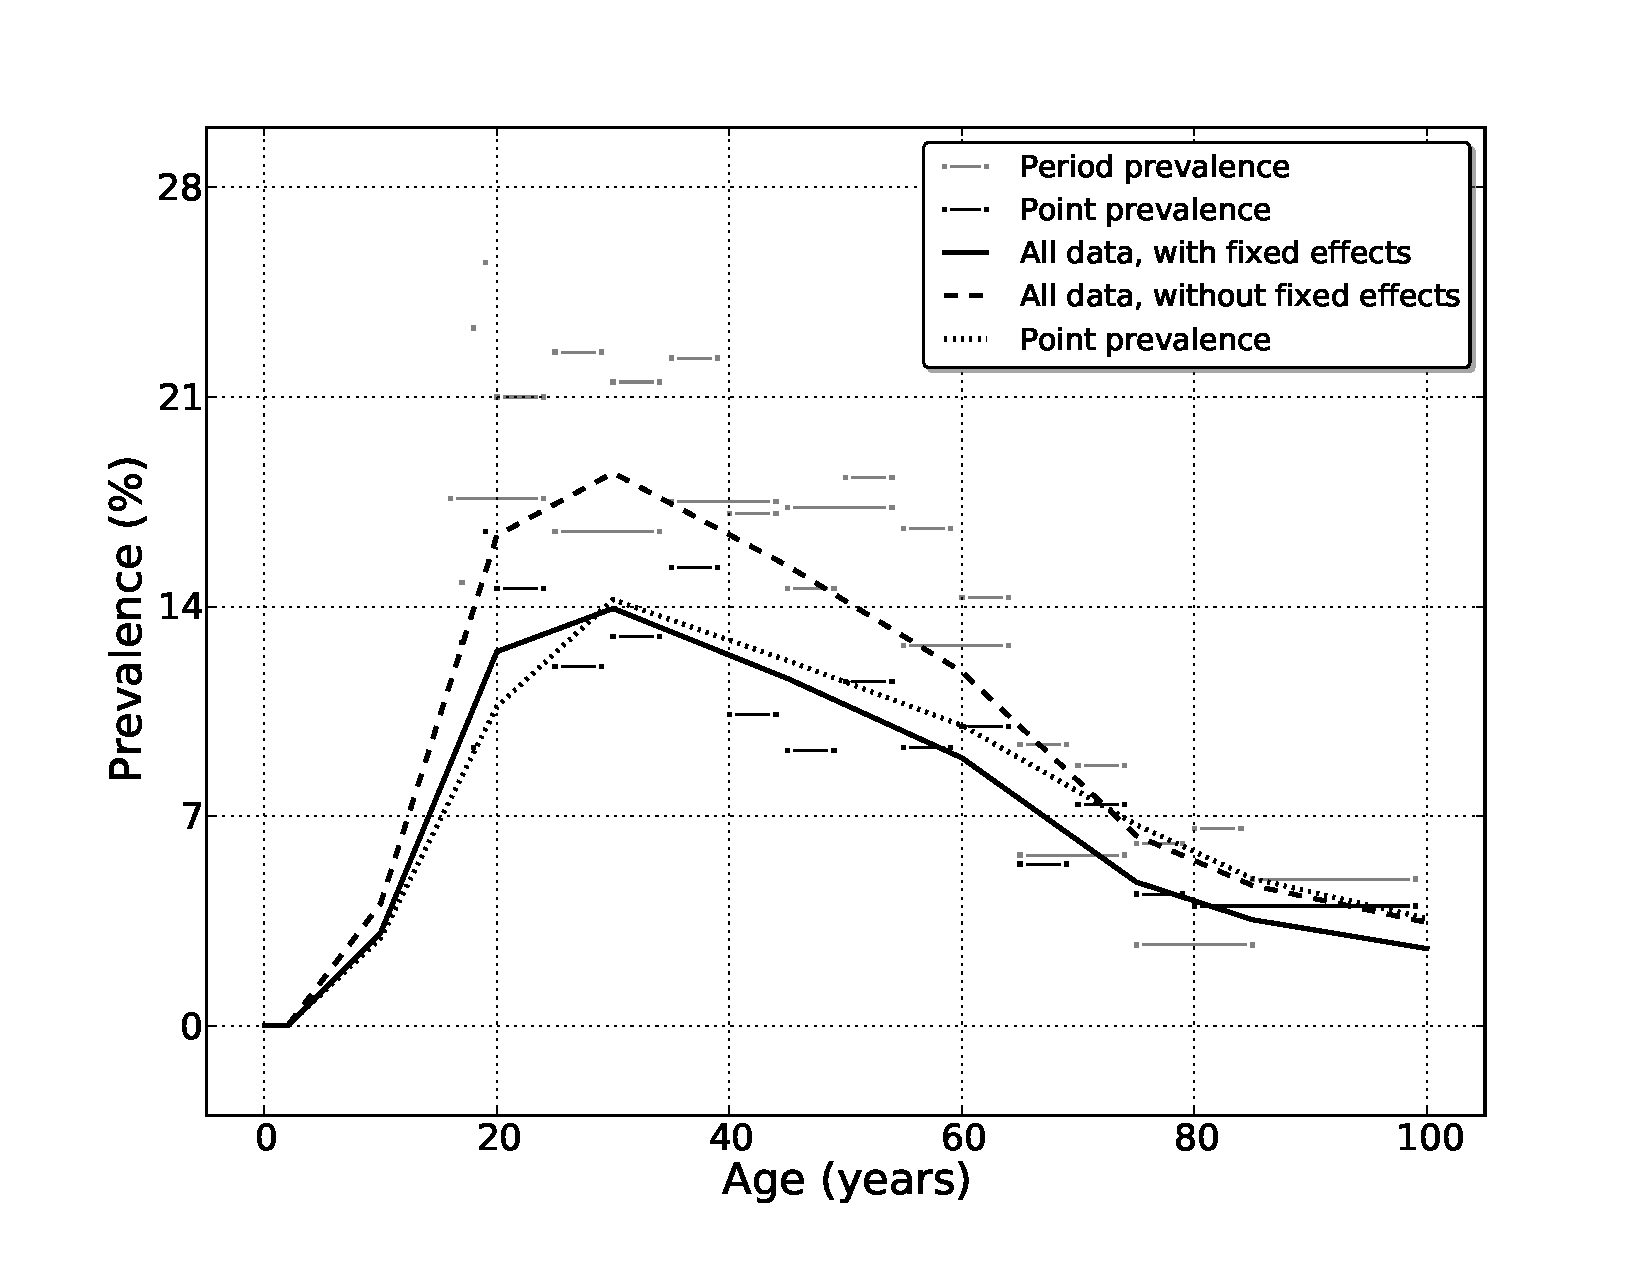
\includegraphics[width=\textwidth]{anxiety-FE.pdf}
            \caption{Comparison of prevalence estimates for anxiety
              disorders in 2005 in Australasian females using point
              prevalence data only, and using point and period prevalence data
              with and without a fixed effect.}
            \label{fig:app-anxiety FE}
        \end{center}
    \end{figure}

The results of the model with a fixed effect on recall period show
that studies on period prevalence typically measure prevalence levels
that are $49$\% (95\% UI: $[12, 91]$) higher than if they measured point
prevalence.

A limitation of applying this method to the global data set is that it
assumes the cross-walk factor is identical for all regions of the
world.  In practice, there is rarely enough data to move beyond this
assumption.  However, future applications may benefit from modeling
interactions between cross-walk covariates and age, sex, time, or
geography.

\chapter{The compartmental model: end-stage renal disease}
\label{applications-fits_incon_v_con}

We now turn our attention to conditions where systematic review
uncovered a substantial amount of nonprevalence data, which we wish
to use to inform our estimates.  This was already touched on in
chapter~\ref{applications-age_groups} and will be investigated more
systematically in the next few chapters.  We begin by considering
end-stage renal disease (ESRD) on dialysis, a condition for which data on
prevalence, incidence, remission, and with-condition mortality were
all collected in relatively large quantities through systematic
review.

ESRD is the final stage of chronic kidney disease (CKD), the slow and
progressive loss of kidney function.  The most common causes of CKD
are diabetes and high blood pressure.  Damage to kidneys is usually
permanent, but treatment and lifestyle changes can slow disease progression.  However, at the final stage of the disease, the kidneys no longer function,
and the patient needs dialysis or a kidney transplant to survive.
There are two main types of
dialysis for kidney treatment: hemodialysis and peritoneal dialysis.
Hemodialysis filters waste and excess fluids from the blood
externally using a machine, while peritoneal dialysis uses the lining
of the peritoneal cavity and a catheter to filter wastes from the
blood. \cite{_k/doqi_2002, dipiro_pharmacotherapy:_2008}

This example focuses on ESRD on dialysis, combining hemodialysis
and peritoneal dialysis for analysis.
Most of the data are from studies or registry reports.
Transplantation incidence among the prevalent
dialysis population was used as a proxy for remission.  The analysis
includes $5664$ data points representing $161$ countries in
all $21$ GBD 2010 Study regions.  Data from Australasia are shown in
figure~\ref{fig:app-CKD data}.
%%   The distribution of dialysis
%% epidemiological parameter data types by region are shown in Table
%% \ref{tab:CKD_data}.


%% \begin{table}[h]
%%     \begin{center}
%%         \caption{ Frequency of dialysis epidemiological parameter data types by region used in analysis}
%%         \label{tab:CKD_data}
%%         \rowcolors{1}{}{gray!50}
%%         \begin{tabular}{|p{3cm}|c|c|c|p{1.5cm}|c|}
%%             \hline
%%                 Region & Prevalence & Incidence & Remission & \centering With-condition mortality & Total \\
%%             \hline
%%                 \raggedright North America, High Income & 277 & 554 & 241 & \centering 240 & 1312 \\
%%                 \raggedright Europe, Western & 362 & 694 & 65 & \centering 10 & 1131 \\
%%                 \raggedright Australasia & 332 & 403 & 144 & \centering 219 & 1098 \\
%%                 \raggedright Asia Pacific, High Income & 161 & 168 & 16 & \centering 26 & 371 \\
%%                 \raggedright Asia, Southeast & 138 & 131 & 14 & \centering 0 & 283 \\
%%                 \raggedright Latin America, Southern & 112 & 113 & 20 & \centering 0 & 245 \\
%%                 \raggedright Asia, East & 107 & 105 & 7 & \centering 0 & 219 \\
%%                 \raggedright Europe, Central & 102 & 86 & 18 & \centering 10 & 216 \\
%%                 \raggedright North Africa Middle East & 76 & 55 & 17 & \centering 2 & 150 \\
%%                 \raggedright Europe, Eastern & 53 & 53 & 13 & \centering 0 & 119 \\
%%                 \raggedright Sub-Saharan Africa, West & 21 & 18 & 51 & \centering 0 & 90 \\
%%                 \raggedright Asia, South  & 35 & 29 & 8 & \centering 0 & 72 \\
%%                 \raggedright Latin America, Tropical & 42 & 10 & 6 & \centering 6 & 64 \\
%%                 \raggedright Sub-Saharan Africa, East & 12 & 9 & 39 & \centering 0 & 60 \\
%%                 \raggedright Latin America, Central & 24 & 21 & 12 & \centering 1 & 58 \\
%%                 \raggedright Caribbean & 15 & 9 & 33 & \centering 0 & 57 \\
%%                 \raggedright Oceania & 13 & 13 & 18 & \centering 0 & 44 \\
%%                 \raggedright Sub-Saharan Africa, Central & 9 & 9 & 18 & \centering 0 & 36 \\
%%                 \raggedright Sub-Saharan Africa, Southern & 6 & 2 & 15 & \centering 0 & 23 \\
%%                 \raggedright Asia, Central & 2 & 1 & 6 & \centering 0 & 9 \\
%%                 \raggedright Latin America, Andean & 5 & 2 & 0 & \centering 0 & 7 \\
%%                 \raggedright Total & 1904 & 2485 & 761 & \centering 514 & 5664 \\
%%             \hline
%%         \end{tabular}
%%     \end{center}
%% \end{table}

    \begin{figure}[h]
        \begin{center}
            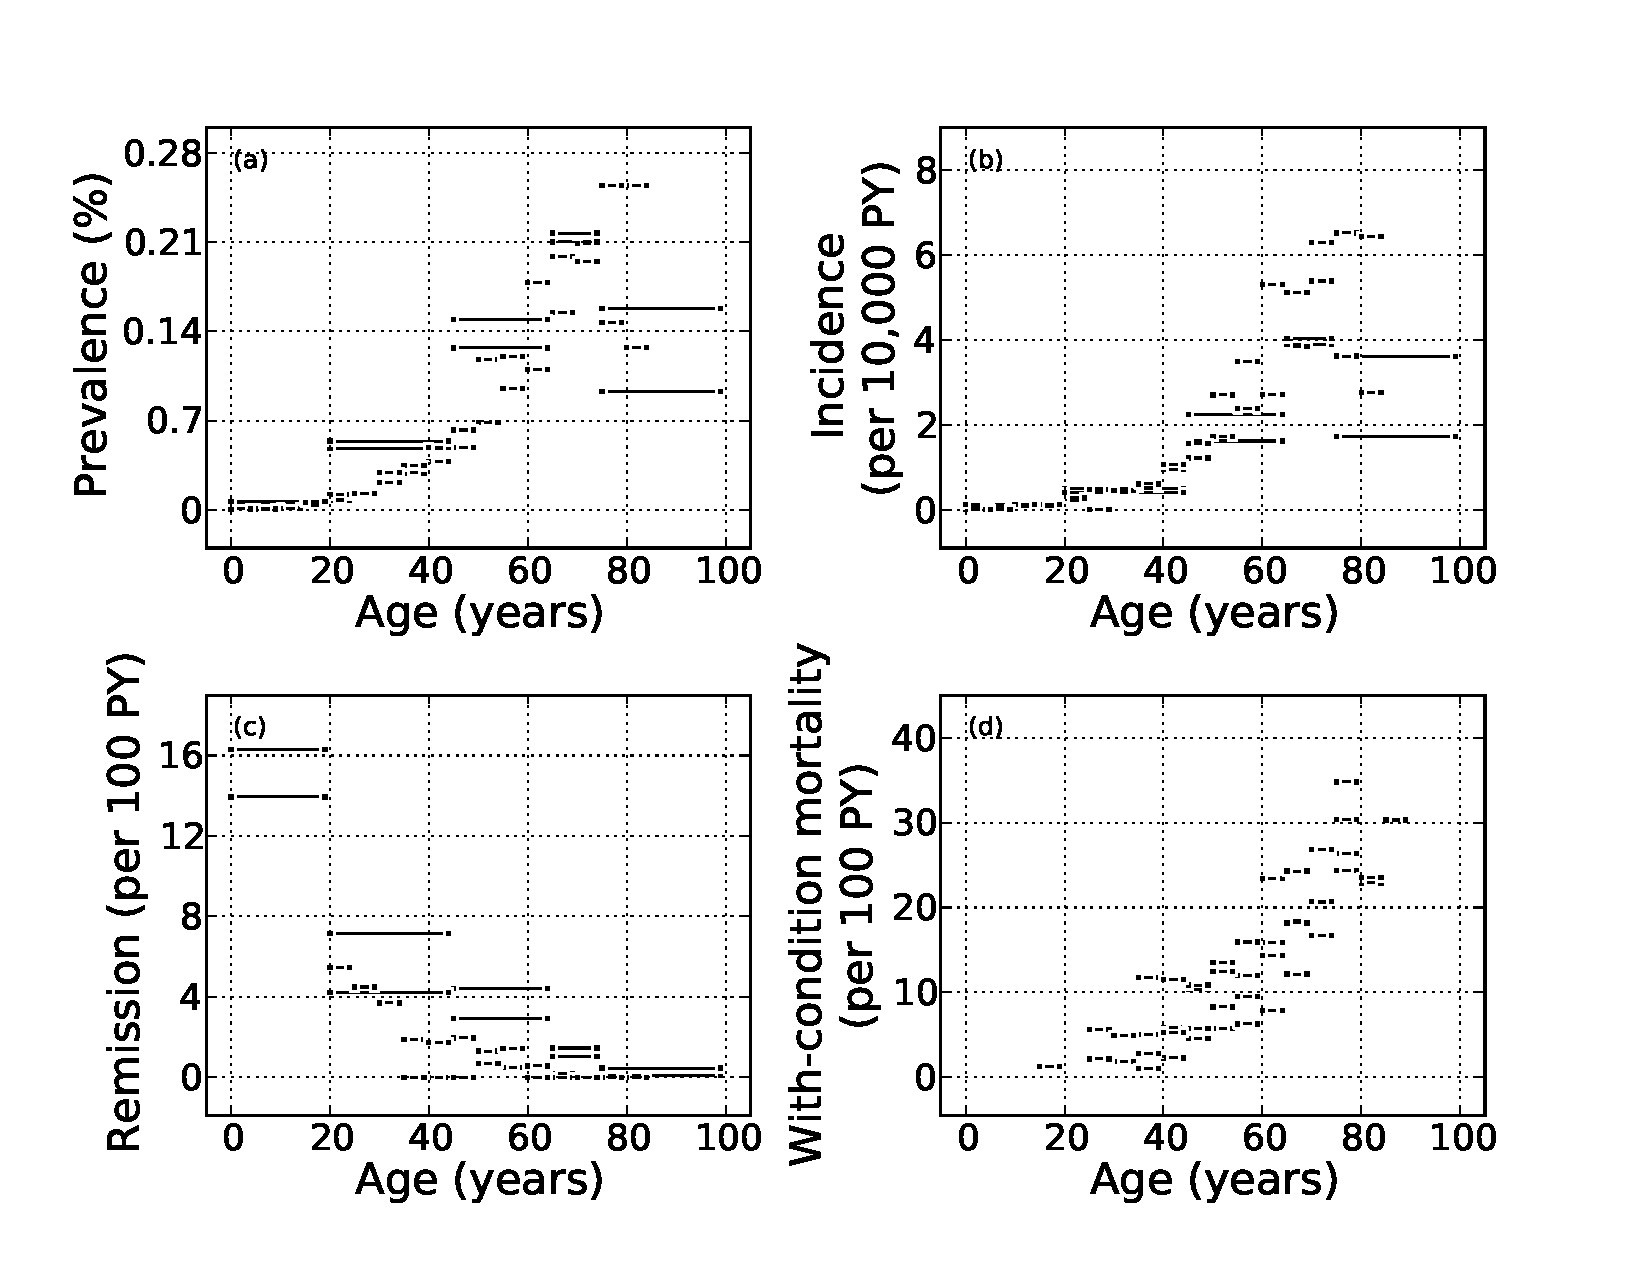
\includegraphics[width=\textwidth]{ckd-data.pdf}
            \caption{Four types of data for Australasian males with ESRD on dialysis
              in 2005: (a) prevalence, (b) incidence, (c)
              remission, and (d) with-condition mortality.}
            \label{fig:app-CKD data}
        \end{center}
    \end{figure}

As discussed in section~\ref{sys-dynamics}, epidemiological parameters,
such as incidence, prevalence, remission, and with-condition
mortality, are related by a logical requirement of internal
consistency.  A prevalence case can exist only if there was a past
incidence event, and the current number of prevalence cases can be
determined from past prevalence cases, new incidence cases, deaths, and
remissions.  Modeling the parameters simultaneously produces a best
estimate and plausible uncertainty bounds for incidence and prevalence
that are internally consistent for a single time, place, and sex.

Figure~\ref{fig:app-CKD incon v con} compares the compartmental and
spline model results for Australasian males with
ESRD on dialysis in 2005.  While the spline model estimates each
epidemiological parameter individually, the compartmental model estimates
prevalence, incidence, remission, and with-condition mortality
simultaneously.  Figure~\ref{fig:app-CKD incon v con} and a
comparison of the age-standardized prevalence estimates for the region
show that the compartmental model estimates do not follow the data
like the spline model does.  As seen in figure~\ref{fig:app-CKD asp}, the
spline model produces prevalence estimates that are systematically lower
than those of the compartmental model because of the logic requirement that
requires all prevalence cases to have a corresponding incidence event.

    \begin{figure}[h]
        \begin{center}
            \includegraphics[width=\textwidth]{ckd-incon_v_con.pdf}
            \caption{Comparison of epidemiological parameter estimates
              for Australasian males with ESRD on dialysis
              in 2005 using the compartmental and spline
              models.}
            \label{fig:app-CKD incon v con}
        \end{center}
    \end{figure}

    \begin{figure}[h]
        \begin{center}
            \includegraphics[width=\textwidth]{ckd-asp_scatter.pdf}
            \caption{Comparison of the regional age-standardized
              prevalence estimates using compartmental and spline
              models for males with ESRD on dialysis in
              2005.}
            \label{fig:app-CKD asp}
        \end{center}
    \end{figure}

Another advantage to compartmental modeling is an estimate with a smooth
age pattern. Modeling each epidemiological parameter individually, the
spline model follows the data exactly, often producing an
uneven age pattern as seen in figure~\ref{fig:app-CKD smooth}.  This
effect can be minimized by placing an informative prior on the
penalized spline model as discussed in chapter~\ref{theory-age_pattern_model}.

    \begin{figure}[h]
        \begin{center}
            \includegraphics[width=\textwidth]{ckd-m_with_smoothing.pdf}
            \caption{With-condition mortality estimates for
              Australasian males with ESRD on dialysis in
              2005 using a compartmental model, a spline model,
              and a spline model with a smoothing parameter.}
            \label{fig:app-CKD smooth}
        \end{center}
    \end{figure}

The compartmental model is preferable to modeling each parameter
individually with the spline model because it incorporates all
available data.  Simultaneously modeling all data, the compartmental
model produces internally consistent estimates for a single age,
sex, and time.

\chapter{Overlapping, heterogeneous age groups: atrial fibrillation}
\label{applications-age_groups}

Like many conditions analyzed in the GBD 2010 Study, Atrial
Fibrillation (AF) has no standard set of age groups for reporting.  The
meta-analysis of the data collected in systematic review must address
these heterogeneous age groups in some way. AF provides a prototypical
example of this, one where the implication of the modeling choices to
use an age-standardizing model can be compared to other possible
choices.  This chapter compares the estimates produced for AF
prevalence and incidence using an age-standardizing model to those
from a midpoint model.

AF is the most common type of cardiac arrhythmia.  Chaotic and
irregular heart rhythms originating in the atria cause poor blood flow
to the body.  The duration of AF episodes vary greatly.  First attacks
or paroxysmal AF are occasional, only lasting a few minutes or hours,
whereas persistent AF and permanent AF are chronic, continuing for
days with or without self-termination.  Symptoms include
heart palpitations, lack of energy, dizziness, shortness of breath and
chest discomfort, although some cases of atrial fibrillation are
symptomless.  AF may occur at any age with increasing risk for older
ages, and is uncommon in children.  Other heart diseases tend to be
the underlying cause of AF.  AF is associated with with coronary heart
disease, hypertensive heart disease, valvular heart disease, heart
failure, cardiomyopathy, obesity and metabolic disorders such as
diabetes and hyperthyroidism. \cite{rich_epidemiology_2009,
  rho_asymptomatic_2005, fuster_acc/aha/esc_2006, radford_atrial_1977,
  TK_ref_from_Mehrdad}

The GBD 2010 Study defines AF as a patient having a least one episode
confirmed by a physician.  The systematic review of AF collected $3942$
data points, of which $247$ were from countries in Western Europe.  We
will consider only the Western European data in this chapter. It
consists of $20$ data points on disease incidence and $147$ on prevalence.
As seen from Figure~\ref{fig:app-af data}, atrial fibrillation has
heterogeneous and overlapping age groups.  Without access to the
microdata needed to recreate homogeneous age groups, combining all of
this data must rely on age group modeling, as described in
Chapter~\ref{chap:age_group_model}.

    \begin{figure}[h]
        \begin{center}
            \includegraphics[width=\textwidth]{af-data.pdf}
            \caption{Data for Western European males with
              AF is an excellent example of heterogeneous
              and overlapping age groups.}
            \label{fig:app-af data}
        \end{center}
    \end{figure}

As discussed in Section~\ref{theory-age_group_model-overlapping_data},
the simplest approach to modeling heterogeneous age groups is to apply
each age-specific rate measurement to the midpoint of the age interval.
Another solution to the heterogeneous age groups is to use age-standardizing.
Age-standardizing adds age weights to the age-specific rate according
to population structure.  The age-standardizing model uses a common
age pattern for all studies so that the age weights are the same for
all country-years, as discussed in more detail in Chapter~\ref{chap:age_group_model}.

As the prevalence estimates in Figure~\ref{fig:app-af srt p} show,
model choice changes the estimates.  In estimates before age 80, 
differences are minimal, but in estimates for older ages, where the
data is sparser and noisier, the differences are substantial.

    \begin{figure}[h]
        \begin{center}
            \includegraphics[width=\textwidth]{af-mp_v_hetero_srt_p.pdf}
            \caption{Comparison of prevalence of AF estimates for Western European
              males in 1990 using an age-standardizing
              or midpoint spline model.  Panel (a) shows the data and
              estimates for the age-standardizing model and panel (b)
              data and estimates for the midpoint model.}
            \label{fig:app-af srt p}
        \end{center}
    \end{figure}

Without additional information, one cannot say which model is preferred.
Further investigation with incidence does not provide much insight.  Like
the prevalence estimates, Figure~\ref{fig:app-af srt i} shows that the
incidence estimates are similar in younger ages, but are markedly different
in older ages.  The age-standardizing model also produces estimates with a
smoother age pattern.

    \begin{figure}[h]
        \begin{center}
            \includegraphics[width=\textwidth]{af-mp_v_hetero_srt_i.pdf}
            \caption{Comparison of incidence of AF estimates for Western European
              males in 1990 using (a) the age-standardizing spline model and (b)
              the midpoint spline model.}
            \label{fig:app-af srt i}
        \end{center}
    \end{figure}

Using all available data in a compartmental model, including the
limited available data on excess mortality, with-condition mortality
and cause-specific mortality, is a way to combine the data on
incidence and prevalence to produce internally consistent estimates by modelling all
parameters simultaneously.  The prevalence estimates from this model
are preferred to a spline model of prevalence alone because it
incorporates additional evidence.  Compartmental models are discussed in
more discussed in more detail in Chapter~\ref{sys-dynamics}.  Figure~\ref{fig:app-af age-stand} shows consistent prevalence and incidence estimates
from the age-standardizing compartmental model.

The compartmental model estimates for incidence in Figure~\ref{fig:app-af age-stand}
are very different from the spline model estimates.
Unlike the spline models, the compartmental model estimates for
incidence do not go through the data.  This is because the compartmental model
requires internal consistency, i.e. for every prevalent case there must be
a matching incident event.  The compartmental model shows that these levels
of prevalence cannot be achieved with the levels of incidence the data show.

    \begin{figure}[h]
        \begin{center}
            \includegraphics[width=\textwidth]{af-best_model.pdf}
            \caption{Estimates of AF prevalence (a) and incidence (b)
              in Western European males in 1990 using
              an age-standardizing compartmental model.}
            \label{fig:app-af age-stand}
        \end{center}
    \end{figure}

Figure~\ref{fig:app-af compare} compares the prevalence and incidence
estimates from the age-standardizing compartmental model to the
midpoint compartmental model.  Like the spline models, the
estimates only differ substantially in the oldest ages.

    \begin{figure}[h]
        \begin{center}
            \includegraphics[width=\textwidth]{af-mp_v_hetero.pdf}
            \caption{A comparison of the estimated prevalence (a) and incidence
              (a) in Western European males with AF in 1990
              using an age-standardizing and midpoint compartmental models.}
            \label{fig:app-af compare}
        \end{center}
    \end{figure}

Choice of age group model has implications for disease estimates.
Estimated age pattern, trends and levels can differ between the
midpoint and age-standardizing models.  A unique feature of the
approach developed in this book is the age-standardizing models, which
result in more appropriate use of systematic review data than simply
applying the measurement to the midpoint of the age interval.

\chapter{Expert priors in compartments models: bipolar disorder}
\label{applications-prior_level_vals}

Just as priors in the spline model were influential on the estimates
produced for PMS prevalence in
Chapter~\ref{applications-priors_knots_select}, the priors on the
age-specific rates in a compartmental model can be influential on the
estimates.  The situation is more complicated here, however, because
priors on a hazard of one type propagate through to affect the
estimates for all other parameters as well, due to the consistency
enforced by the compartmental model.  In this chapter, we will use the
meta-analysis of bipolar disorder prevalence as an example of the
effects of informative priors on levels of age-specific incidence and
remission hazards.

Bipolar disorder is a mental disorder that causes the experience
of at least one manic and one major depressive episode,
interspersed by periods of residual symptoms.  A manic episode is
characterized by elevated, expansive, or irritable mood while a
depressive episode is characterized by depressed mood or loss of
interest in everyday activities.  A shift between episodes is
demarcated by either a change in symptoms to the opposite polarity
or experiences of residual symptoms which are below the threshold
for a manic or depressive episode.  In the case of rapid cycling,
shifts between episodes occur as frequently as four or more shifts
in a given year.  Extreme behavior
changes accompany mood changes, and it is not uncommon for sleeping,
eating or activity patterns to change with manic and depressive
episodes.
While there
is no cure, treatment helps manage mood swings and related
symptoms. \cite{kloos_bipolar_2011, angst_historical_2000, TK_coauthor_ref}

The modeling of bipolar disorder is based on literature describing it
as a chronic illness with little or no complete remission.
The terms ``residual'' and ``remission'' have very different implications
for the GBD 2010 study.  A residual state involves less severe
symptoms with lesser disability which still contributes to disease
burden.  Remission is equivalent to a cure rather than a temporary
reduction in symptom levels, thus not contributing to burden.  No studies
were found reporting on complete remission from bipolar disorder as per this definition,
which is consistent with the description in the literature that there
is no cure. \cite{american_psychiatric_association_diagnostic_2000}
In this chapter, analysis
only uses data from the GBD 2010 Study region of North America, High Income,
shown in Figure~\ref{fig:app-bipolar data}.

    \begin{figure}[h]
        \begin{center}
            \includegraphics[width=\textwidth]{bipolar-data.pdf}
            \caption{Data collected from systematic review of bipolar
              disorder of (a) prevalence, (b) incidence, (c) remission and
              (d) standardized mortality ration in the GBD 2010 Study
              region of North America, High Income.}
            \label{fig:app-bipolar data}
        \end{center}
    \end{figure}

%\section{Prevalence and Incidence age of onset}
While there is evidence to suggest that bipolar disorder commonly
starts in the mid-teens or early twenties, there is still disagreement
over a minimum age of onset.  Even though symptoms can be tracked back
to childhood, setting a threshold for diagnosis is difficult given
that current diagnostic criteria are based on the adult presentation of
the disorder.  Literature and expert advice suggest that although
pre-pubertal bipolar disorder is rare, there is a possibility it may
exist. \cite{kloos_bipolar_2011, angst_historical_2000}

While expert priors are useful in guiding the modeling process, they
may have unintended effects as discussed in Chapter~\ref{theory-expert_priors}.
Choosing to have no restrictions on the
age of onset, the age-specific prevalence differs greatly, as shown in
Figure~\ref{fig:app-bipolar bounds}.

    \begin{figure}[h]
        \begin{center}
            \includegraphics[width=\textwidth]{bipolar-bounds.pdf}
            \caption{Estimates of the prevalence of bipolar disorder
              for males in the GBD 2010 Study region of North America, High Income
              in 1990 using differing priors that limit the age of onset
              in a compartmental model.}
            \label{fig:app-bipolar bounds}
        \end{center}
    \end{figure}

Like the age of onset, little is known about the upper age limit of
bipolar disorder.  Using expert knowledge to set plausible bounds on the
level of disease is useful in modeling noisy data.  However, changes in the upper age
limit may produce unexpected changes as shown in Figure~\ref{fig:app-bipolar onset}.
The prevalence estimates in Figure~\ref{fig:app-bipolar onset} are about
the same because there is enough data to inform the model, but incidence,
remission and excess mortality make subtle changes to account for the prior.

    \begin{figure}[h]
        \begin{center}
            \includegraphics[width=\textwidth]{bipolar-45_65_100.pdf}
            \caption{Estimated (a) prevalence, (b) incidence, (c) remission and
              (d) excess mortality for males with bipolar
              disorder in the GBD 2010 Study region of North America, High Income
              in 1990 using a compartmental model with
              different priors that restrict the upper age limit of
              incidence to 45, 65 or 100.}
            \label{fig:app-bipolar onset}
        \end{center}
    \end{figure}

%\section{Residual v Remission}
In sparse and noisy data, sometimes the changes to account for the prior
are not so subtle, as shown in the sensitivity analysis in
Figure~\ref{fig:app-bipolar remission}.  Here, small changes in the
prior level on remission lead to large changes in the estimated excess mortality.

    \begin{figure}[h]
        \begin{center}
            \includegraphics[width=\textwidth]{bipolar-0_5_10.pdf}
            \caption{Estimated (a) remission and (b) excess
              mortality for bipolar disorder in
              males in the GBD 2010 Study region of North America, High Income
              in 1990 in a compartmental model
              with different priors on remission which limit remission
              to 0, 5 or 10 per 100 PY.}
            \label{fig:app-bipolar remission}
        \end{center}
    \end{figure}

The internal consistency in the compartmental model causes modeling
decisions, such as priors on level, for one parameter to propagate and
affect all other parameter estimates.  When working with ample data,
the model estimates are robust to the choice of informative priors on
level.  However, these choices can cause substantial changes to
estimates when working with sparse and noisy data.





\chapter{Short duration conditions: diarrheal diseases}
\label{applications-short_dur}

Diarrheal diseases are a leading cause of childhood morbidity and mortality.  Typically defined as having loose or watery stools three or more times a day or more frequently than normal for the individual, the diarrheal episodes typically last 1-8 days for acute cases depending on severity \cite{unicef_diarrhoea_2009, carlos_etiology_1990, lamberti_systematic_2012}.  Compared to many of the other diseases discussed thus far, diarrheal diseases have a very short duration.

Bacterial, viral and parasitic infections cause most cases of intestinal infectious diarrhea.  Typically spread via the oral-fecal route, water sanitation and hygiene is a large part of diarrhea prevention.  Treatment usually involves fluid replacement, as acute diarrhea causes fluid loss and dehydration.  Other common treatments are vitamin A and zinc supplementation, vaccinations and antibiotic regimes \cite{unicef_diarrhoea_2009, carlos_etiology_1990, lamberti_systematic_2012}.

For the analysis of diarrheal diseases, the primary sources of data are from surveys, hospital admissions and literature review.  The surveys report period prevalence data whereas hospital admissions and the majority of the literature report incidence data.  In short term diseases, point prevalence and incidence are approximately the same.  Therefore to avoid compositional bias, all incidence and period prevalence estimates were converted to point prevalence estimates using the assumption that
    \begin{equation}
    	p_{point}=i*d
    \end{equation}
where $p_{point}$ is the point prevalence, $i$ is the incidence and $d$ is the duration of the disease.  Thus the analysis includes 2029 rows of prevalence data from 19 regions.  Data from Central Latin America is shown in Figure \ref{fig:app-diarrhea data}.  Cause-specific mortality assumes that anyone with the disease died of the disease.

    \begin{figure}[h]
        \begin{center}
            \includegraphics[width=\textwidth]{diarrhea-data.pdf}
            \caption{Diarrheal point prevalence (panel (a)) and cause-specific mortality (panel (b)) data in Central Latin America.}
            \label{fig:app-diarrhea data}
        \end{center}
    \end{figure}

Diarrheal diseases use a compartmental model to model all epidemiologic parameters for a single time, place and sex.  A compartmental model estimates all epidemiologic parameters simultaneously which maintains internally consistent results as discussed in Chapters \ref{sys-dynamics} and \ref{applications-fits_incon_v_con}.  In addition to the systematic review data, informative priors on the duration of diarrheal diseases help guide the modeling process.  The prior for duration is set as the prior for remission.  Duration priors produce less stable estimates than the more directly parameterized remission priors.  Therefore remission is the more appropriate prior for the model.  Equation \ref{eq:remission-duration} approximates the relationship between duration and remission
    \begin{equation} \label{eq:remission-duration}
    	r = \frac{1}{d}
    \end{equation}
where $r$ is the epidemiologic rate for remission and $d$ is the epidemiologic rate for duration in years.  Similar to the discussion of priors in Chapter \ref{applications-con_fit_splines}, the choice of priors affects the epidemiological estimates.  However, because of the logical requirement of internal consistency, a change in the duration of diarrheal diseases has effects on all epidemiological parameters as seen in Figure \ref{fig:app-diarrhea duration}.

    \begin{figure}[h]
        \begin{center}
            \includegraphics[width=\textwidth]{diarrhea-duration.pdf}
            \caption{Estimates of prevalence (panel (a)), incidence (panel (b)), remission (panel (c)) and excess-mortality (panel (d)) for diarrheal diseases in Central Latin American males in 2005 using a compartmental model with differing priors on disease duration, $d$.}
            \label{fig:app-diarrhea duration}
        \end{center}
    \end{figure}

\chapter{Liver Cirrhosis}
\label{applications-efx_country_level}

Besides explaining the bias of noisy measurement as discussed in Chapter \ref{applications-efx_study_level}, fixed effects can also increase the accuracy of out-of-sample predictions.  By modeling the relationship between the epidemiologic parameter of interest and an explanatory covariate, extrapolation can predict epidemiologic parameters in areas where no epidemiologic parameter measurements are available but covariate data are.  Few regions have epidemiologic measurements for liver cirrhosis.  However, by using the age-standardized hepatitis C prevalence as a country-level covariate to predict out-of-sample, it is possible to estimate the prevalence of cirrhosis.

As the result of chronic liver injury, liver cirrhosis is an advanced stage of liver scarring.  Cirrhosis is the end stage of any chronic liver disease, with the most common causes being alcoholic liver disease and hepatitis B and C.  Asymptomatic during the early stages of the disease, compensated cirrhosis may go undetected until complications develop.  The diagnostic gold standard for cirrhosis is a liver biopsy.  Complications such as portal hypertension, jaundice, ascites, gastrointestinal bleeding and liver dysfunction mark the progression from compensated to decompensated cirrhosis.  Irreversible, cirrhosis management is the prevention, control and treatment of cirrhosis complications, with liver transplantation being the ultimate treatment.  Without a liver transplant, cirrhosis mortality is very high \cite{garcia-tsao_management_2009, d'amico_natural_2006, schuppan_liver_2008}.

Systematic review yielded prevalence and cause-specific mortality rate estimates from four (of 21 possible) regions.  Given the difficulty in cirrhosis diagnosis, it is assumed this data represents decompensated cirrhosis and the following analysis focuses on the decompensated phase of the disease, assuming almost all prevalent cases lead to death.

    \begin{figure}[h]
        \begin{center}
            \includegraphics[width=\textwidth]{cirrhosis-data.pdf}
            \caption{Available global data for cirrhosis prevalence (a) and cause-specific mortality (b).}
            \label{fig:app-cirrhosis data}
        \end{center}
    \end{figure}

Since cirrhosis is so deadly, it is a reasonable assumption that regions with increased deaths from cirrhosis also have increased cirrhosis prevalence.  Figure \ref{fig:app-cirrhosis asp} shows the relationship between the natural log of the age-standardized death rate of cirrhosis and cirrhosis prevalence.

    \begin{figure}[h]
        \begin{center}
            \includegraphics[width=\textwidth]{cirrhosis-lnASDR_v_prev.pdf}
            \caption{Relationship between the natural log of the age-standardized death rate of cirrhosis and cirrhosis prevalence.}
            \label{fig:app-cirrhosis asp}
        \end{center}
    \end{figure}

In regions with no liver cirrhosis data, estimates of the age-standardized cirrhosis death rate may be used as an explanatory covariate to estimate cirrhosis prevalence.  By borrowing strength from the mortality estimates to inform the incidence estimates, cirrhosis prevalence can be estimated for regions without data as shown in figure \ref{fig:app-cirrhosis prev est}.

    \begin{figure}[h]
        \begin{center}
            \includegraphics[width=\textwidth]{cirrhosis-lnASDR_v_prev.pdf}
            \caption{.}
            \label{fig:app-cirrhosis prev est}
        \end{center}
    \end{figure}

\chapter{Missing epidemiological parameter data: transport injuries}
\label{applications-double_dismod}

For whatever reason, data are often not available for one or more
epidemiological parameters.  In the GBD 2010 study, this is
problematic when the missing parameter is needed for the calculation
of disease burden.  Injuries provide an excellent example of missing
epidemiological parameter data as incidence is often only reported.

In the GBD 2010 Study, injuries are defined as conditions codable to
the ICD-9 and ICD-10 injuries chapter.  Transport injuries includes
all road injuries for pedestrian, bicyclist, motorized two-wheeler
rider, occupant in a motorized vehicle with 3 or more wheels, other
road-transport injury and unintentional other transport injury.

Data only include cases warranting hospital care and cases warranting
treatment by health care professional but not hospitalization (other
health care).  As seen in Figure \ref{fig:app-injury traffic data},
only incidence and cause-specific mortality were available from verbal
autopsy, surveillance systems, surveys, census and police reports.
Cause-specific mortality assumes that anyone who died with the
condition died of the condition.

    \begin{figure}[h]
        \begin{center}
            \includegraphics[width=\textwidth]{injury-traffic_data.pdf}
            \caption{Incidence (panel (a)) and cause-specific
              mortality (panel (b)) data for transport injuries for
              males in the region of North America, High Income.}
            \label{fig:app-injury traffic data}
        \end{center}
    \end{figure}

To estimate prevalence, both the cause-specific mortality and the
incidence data are used in a compartmental model to estimate the
age-specific burden of transport injuries, as shown in Figure
\ref{fig:app-injury traffic fit}.  By fitting all of the epidemiological
parameters together, the compartmental model can estimate prevalence
without prevalence data.

    \begin{figure}[h]
        \begin{center}
            \includegraphics[width=\textwidth]{injuries-traffic_con_fit.pdf}
            \caption{A compartmental model estimates the prevalence
              (panel (a)), incidence (panel (b)), cause-specific
              mortality (panel (c)) and with-condition mortality
              (panel (d)) for males in the United States of America in
              2005.}
            \label{fig:app-injury traffic fit}
        \end{center}
    \end{figure}

For most conditions, this is all that is necessary to calculate
disease burden.  However, transport injuries have a wide range of
outcomes, ranging from minor scratches to severe brain trauma to
death.  Given some cases suffer acute injury while others sustain
chronic conditions, the burden of the disease and the mortality hazard
differ by outcome.  Thus the compartmental model is not appropriate
for traffic injuries since it violates the model assumption of a
constant mortality hazard.  To address this disparity in mortality
risk, transport injuries can be divided into short term and long term
outcomes.  This method is also necessary for other injuries and
diseases such as heart attack and stroke.

Dividing incidence into short and long term outcomes avoids violating
the assumption of a constant mortality hazard.  Once long term traffic
injury incidence is extracted, it is further subdivided into the
nature of the injury, such as fractures, burns, amputations or
traumatic brain injury.  Systematic review only yields traumatic brain
injury incidence.  Again, the compartmental model simultaneously fits
all epidemiological parameters to estimate traumatic brain injury
prevalence, as see in Figure \ref{fig:app-injury brain fit}.

    \begin{figure}[h]
        \begin{center}
            \includegraphics[width=\textwidth]{injuries-con_fit_p.pdf}
            \caption{Prevalence (panel (a)) and incidence (panel (b))
              estimates for males in the United States of America in
              2005 with moderate to severe traumatic brain injury
              caused by traffic injuries.}
            \label{fig:app-injury brain fit}
        \end{center}
    \end{figure}




\chapter{Empirical priors: visceral leishmaniasis}
\label{applications-priors_empirical}

Moving away from more `subjective' expert priors, empirical priors
rely on the data.  Similar to fitting the complete hierarchical model,
empirical priors use predictions from a simple global model to inform
parallel regional models, as discussed in Chapter
\ref{theory-age_pattern_model}.  In modeling diseases with
insufficient data for all geographic areas, such as visceral
leishmaniasis (VL), empirical priors provide data-derived
relationships to guide the modeling process.

VL is a parasitic disease in which the parasite
invades cells in the liver, spleen, bone marrow and lymph nodes.  If
untreated, it causes life-threatening systemic infection.  Diagnosis
includes identification of the parasite in tissue samples, ideally
from the spleen or bone marrow.  The parasite is transmitted by
several species of sandflies.  Traditionally endemic in the tropics,
subtropics and southern Europe, VL is becoming an AIDS-associated
opportunistic infection. \cite{herwaldt_leishmaniasis_1999,
baron_medical_1996}

Data are primarily from hospital admissions records, but also include
a handful of published studies.  Only population
representative data were included for the analysis, specific
population groups and cases of HIV-coinfection were excluded.  Thus
the analysis includes $3583$ data points from $12$ GBD 2010 study regions.

    \begin{figure}[h]
        \begin{center}
            \includegraphics[width=\textwidth]{vl-data.pdf}
            \caption{Visceral leishmaniasis incidence data from
              systematic review for GBD 2010 study.  Data from Latin
              America and the Caribbean are shown in panel (a), and
              data sub-Saharan Africa are shown in panel (b).  The
              levels of the data are extremely heterogeneous; note
              that even displaying them requires a log-scale on the
              $y$-axis.}
            \label{fig:app-vl data}
        \end{center}
    \end{figure}

The data from the cluster of regions composed of the Caribbean,
central, Andean and tropical Latin America, has low incidence.
However it has an age-pattern that can be used as an empirical prior
for areas without an age-pattern, such as the regions in sub-Saharan
Africa.  Figure \ref{fig:app-vl data} shows the available data for
these clusters of regions.

Estimates using only data from sub-Saharan Africa alone would have no
way to estimate the age pattern of disease incidence. By borrowing
strength from the Latin America region cluster, it is possible.  The
empirical bayes approach to this is shown in Figure \ref{fig:app-vl
  pred compare}.

    \begin{figure}[h]
        \begin{center}
            \includegraphics[width=\textwidth]{vl-pred_compare.pdf}
            \caption{A comparison of incidence estimates for males in
              super-region 6 (panel (a)) and super-region 2 (panel
              (b)) using data solely from that geographical area, data
              from both areas and data solely from that area with the
              estimate from both areas as an empirical prior.}
            \label{fig:app-vl pred compare}
        \end{center}
    \end{figure}



\bibliographystyle{plainnat}
\bibliography{my_library}
\end{document}
